% !TeX document-id = {f3146876-9a53-4f56-9560-e6295d649f82}
% !TeX program = pdflatex
% !TeX TXS-program:bibliography = txs:///biber
% !TeX encoding = utf8


\documentclass{utthesis}

% If you use luatex (better)
% \usepackage[utf8]{inputenc}

\usepackage[%
	backend=biber,
	style=ieee,
	maxbibnames=4,
	minbibnames=1,
	maxcitenames=3,
	mincitenames=1,
	backref=true
	]{biblatex}

\addbibresource{references.bib}

\usepackage{lipsum} % Dummy text for examples
\usepackage{graphicx}
\usepackage{slashed}
\usepackage{xspace}
\usepackage{amssymb}
\usepackage{multirow}
\usepackage{arydshln, array}



%%%%%%%%%%%%%%%%%%%%%%%%%%%%%%%%%%%%%%%%%%%%%%%%%%
% These are some new commands that may be useful 
% for paper writing in general. If other newcommands
% are needed for your specific paper, please feel 
% free to add here. 
%
% The currently available commands are organized in: 
% 1) Systems
% 2) Quantities
% 3) Energies and units
% 4) Detectors
% 5) particle species 
%%%%%%%%%%%%%%%%%%%%%%%%%%%%%%%%%%%%%%%%%%%%%%%%%%

% 1) SYSTEMS 
\newcommand{\pp}           {pp\xspace}
\newcommand{\ppbar}        {\mbox{$\text {p\overline{p}}$}\xspace}
\newcommand{\XeXe}         {\mbox{Xe--Xe}\xspace}
\newcommand{\PbPb}         {\mbox{Pb--Pb}\xspace}
\newcommand{\pA}           {\mbox{pA}\xspace}
\newcommand{\pPb}          {\mbox{p--Pb}\xspace}
\newcommand{\AuAu}         {\mbox{Au--Au}\xspace}
\newcommand{\dAu}          {\mbox{d--Au}\xspace}

% 2) QUANTITIES 
\newcommand{\s}            {\ensuremath{\sqrt{s}}\xspace}
\newcommand{\snn}          {\ensuremath{\sqrt{s_{\text{NN}}}}\xspace}
\newcommand{\pt}           {\ensuremath{p_{\text{T}}}\xspace}
\newcommand{\ptlambda}           {\ensuremath{p_{\text T}^{\Lambda}}\xspace}
\newcommand{\pttrig}           {\ensuremath{p_{\text{T}}^{\text{trig.}}}\xspace}
\newcommand{\ptassoc}           {\ensuremath{p_{\text{T}}^{\text{assoc.}}}\xspace}
\newcommand{\meanpt}       {$\langle p_{\text{T}}\rangle$\xspace}
\newcommand{\ycms}         {\ensuremath{y_{\text CMS}}\xspace}
\newcommand{\ylab}         {\ensuremath{y_{\text lab}}\xspace}
\newcommand{\etarange}[1]  {\mbox{$\left | \eta \right |~<~#1$}}
\newcommand{\yrange}[1]    {\mbox{$\left | y \right |~<~#1$}}
\newcommand{\dndy}         {\ensuremath{\text{d}N_\mathrmfamily{ch}/\mathrmfamily{d}y}\xspace}
\newcommand{\dndeta}       {\ensuremath{\text{d}N_\mathrmfamily{ch}/\mathrmfamily{d}\eta}\xspace}
\newcommand{\avdndeta}     {\ensuremath{\langle\dndeta\rangle}\xspace}
\newcommand{\dNdy}         {\ensuremath{\text{d}N_\mathrmfamily{ch}/\mathrmfamily{d}y}\xspace}
\newcommand{\Npart}        {\ensuremath{N_\text{part}}\xspace}
\newcommand{\Ncoll}        {\ensuremath{N_\text{coll}}\xspace}
\newcommand{\dEdx}         {\ensuremath{\texttext{d}E/\textrmfamily{d}x}\xspace}
\newcommand{\RpPb}         {\ensuremath{R_{\text pPb}}\xspace}
\newcommand{\zvtx}         {\ensuremath{Z_{\text vtx.}}\xspace}

% 3) ENERGIES, UNITS
\newcommand{\nineH}        {$\sqrt{s}~=~0.9$~Te\kern-.1emV\xspace}
\newcommand{\seven}        {$\sqrt{s}~=~7$~Te\kern-.1emV\xspace}
\newcommand{\twoH}         {$\sqrt{s}~=~0.2$~Te\kern-.1emV\xspace}
\newcommand{\twosevensix}  {$\sqrt{s}~=~2.76$~Te\kern-.1emV\xspace}
\newcommand{\five}         {$\sqrt{s}~=~5.02$~Te\kern-.1emV\xspace}
\newcommand{\twosevensixnn}{$\sqrt{s_{\text{NN}}}~=~2.76$~Te\kern-.1emV\xspace}
\newcommand{\fivenn}       {$\sqrt{s_{\text{NN}}}~=~5.02$~Te\kern-.1emV\xspace}
\newcommand{\LT}           {L{\'e}vy-Tsallis\xspace}
\newcommand{\GeVc}         {Ge\kern-.1emV/$c$\xspace}
\newcommand{\MeVc}         {Me\kern-.1emV/$c$\xspace}
\newcommand{\TeV}          {Te\kern-.1emV\xspace}
\newcommand{\GeV}          {Ge\kern-.1emV\xspace}
\newcommand{\MeV}          {Me\kern-.1emV\xspace}
\newcommand{\GeVmass}      {Ge\kern-.2emV/$c^2$\xspace}
\newcommand{\MeVmass}      {Me\kern-.2emV/$c^2$\xspace}
\newcommand{\lumi}         {\ensuremath{\mathcal{L}}\xspace}

% 4) DETECTORS 
\newcommand{\ITS}          {\text{ITS}\xspace}
\newcommand{\TOF}          {\text{TOF}\xspace}
\newcommand{\ZDC}          {\text{ZDC}\xspace}
\newcommand{\ZDCs}         {\text{ZDCs}\xspace}
\newcommand{\ZNA}          {\text{ZNA}\xspace}
\newcommand{\ZNC}          {\text{ZNC}\xspace}
\newcommand{\SPD}          {\text{SPD}\xspace}
\newcommand{\SDD}          {\text{SDD}\xspace}
\newcommand{\SSD}          {\text{SSD}\xspace}
\newcommand{\TPC}          {\text{TPC}\xspace}
\newcommand{\TRD}          {\text{TRD}\xspace}
\newcommand{\VZERO}        {\text{V0}\xspace}
\newcommand{\VZEROA}       {\text{V0A}\xspace}
\newcommand{\VZEROC}       {\text{V0C}\xspace}
\newcommand{\Vdecay} 	   {\ensuremath{V^{0}}\xspace}

% 4) PARTICLE SPECIES 
\newcommand{\ee}           {\ensuremath{e^{+}e^{-}}} 
\newcommand{\pip}          {\ensuremath{\pi^{+}}\xspace}
\newcommand{\pim}          {\ensuremath{\pi^{-}}\xspace}
\newcommand{\kap}          {\ensuremath{\text{K}^{+}}\xspace}
\newcommand{\kam}          {\ensuremath{\text{K}^{-}}\xspace}
\newcommand{\pbar}         {\ensuremath{\text\overline{p}}\xspace}
\newcommand{\kzero}        {\ensuremath{{\text K}^{0}_{\rmfamily{S}}}\xspace}
\newcommand{\lmb}          {\ensuremath{\Lambda}\xspace}
\newcommand{\almb}         {\ensuremath{\overline{\Lambda}}\xspace}
\newcommand{\Om}           {\ensuremath{\Omega^-}\xspace}
\newcommand{\Mo}           {\ensuremath{\overline{\Omega}^+}\xspace}
\newcommand{\X}            {\ensuremath{\Xi^-}\xspace}
\newcommand{\Ix}           {\ensuremath{\overline{\Xi}^+}\xspace}
\newcommand{\Xis}          {\ensuremath{\Xi^{\pm}}\xspace}
\newcommand{\Oms}          {\ensuremath{\Omega^{\pm}}\xspace}
\newcommand{\degree}       {\ensuremath{^{\text o}}\xspace}

% This should be the last package you load
\usepackage[hidelinks]{hyperref} % Handy for links, can comment for plain PDF

% Uncomment to use the lineno package to number lines
\usepackage{lineno}
\linenumbers

\UTyear=2023

\makeindex

\graphicspath{{./figures/}}

\errorcontextlines 10000

\begin{document}

\author{Ryan Patrick Hannigan} 
\title{Stranger Things at the LHC}
\date{Revised: \today}

\frontmatter

\UTcopyrightlegend % Optional

\begin{UTcommittee}
\UTaddsupervisor{Christina Markert}
\UTaddcommittee{Peter Onyisi}
\UTaddcommittee{Aaron Zimmerman}
\UTaddcommittee{Chandrajit Bajaj}
\end{UTcommittee}

\UTtitlepage{Ph.D.}{May}

\setcounter{page}{4}


\UTdedication{To Jaynee.}

\chapter{Acknowledgements}

\footnotesize
As it turns out, completing a dissertation is \textit{a lot} of work. I am eternally grateful to the large number of people who have helped me along the way, and without whom this work would not have been possible. I can assure you if I were to properly thank everyone who has helped me, this acknowledgements section would be longer than the ``systematic studies'' chapter of this dissertation. So, I will try to keep it brief, but even by virtue of you reading this sentence, you have my sincerest thanks.

To my advisor, Professor Christina Markert, for her guidance and support throughout my graduate career. I am grateful for the opportunity to have worked with her, and for all of the time and effort she has put into helping me succeed, both as a graduate student \textit{and} as a scientist. To Amanda and Josey, who have had to share an office with me for most of their time at UT. I appreciate all of the conversations and friendship we've shared over the years. To Erin and Alex, who welcomed me into the group and immediately made me feel at home. To Professor Deepa Thomas, who works harder than anyone I have ever met, and yet \textit{somehow} still managed to find time to answer my endless questions. To Lanny, who always made me \textit{believe} I'm capable of understanding the theory of our field. I'm not, but he still made me feel like I could. To Justin, who I've spent more time bugging in his office about random puzzles than I've spent writing this document. His seemingly infinite patience and willingness to help me with my many, many struggles has been invaluable.

To all of the friends I made within the UT Counter Strike community. Without them, I would have finished this dissertation \textit{much} sooner, but all of the memories we've made over the years have been well worth it. To Devanshu and Richard, who would brighten up my day with horrible puns and surprise visits to my office. To my roommates Travis, Kevin and Luke, whose friendship has pulled me through some of the most stressful times. To Matteo, Arild, Matthias and Jo, who converted me from someone who had never heard the acronym ``ssh'' into a full-fledged computer nerd. Without their endless support during my times at CERN, I would have been completely lost. 

To my family, especially my parents and sister, whose love and support during this entire process (a.k.a. my life) cannot be overstated. Their encouragement and belief in me as I pursue my passions has been a constant source of strength. To my fiance\'e Jaynee, who has given me enough happiness and love to last a lifetime, which is \textit{just} enough to offset the stress and anxiety of writing a dissertation. I am so very much excited to spend the rest of my life with her. To Jaynee's family, who have welcomed me into their family with open arms and given me plenty of indispensable guidance during these past few years.

\normalsize
%\include{preface}

\begin{UTabstract}*[]{Christina Markert}
    Quantum chromodynamics (QCD) is the branch of fundamental particle physics that studies the strong interaction, which is responsible for binding quarks and gluons into the familiar protons and neutrons that compose almost all ordinary matter. One of the most exciting predictions of this theory is the existence of a new state of matter, known as the quark-gluon plasma (QGP). At extreme temperatures and densities, protons and neutrons dissolve into their constituent quarks and gluons, forming a soup-like plasma of deconfined partons. This QGP is thought to have existed in the early universe, thus studying its formation and properties can help answer questions about the evolution of the universe and the nature of the strong force. However, recreating the extreme conditions of the early universe requires smashing together heavy nuclei at \textit{very} high energies. This can only be done at the world's most powerful particle accelerators, making the QGP the most expensive soup on the menu.

Unfortunately, producing the QGP in these heavy ion collisions has a major drawback; it is only created for around $10^{-23}$ seconds, making it impossible to study directly with a detector. Instead, there are a few key experimental observables that are associated with the formation of this plasma which can be studied in a detector. One such signature of QGP formation is known as strangeness enhancement, where the production of strange quarks within the QGP is enhanced relative to the standard up and down quarks that compose protons and neutrons. Previously believed to be unique to heavy ion collisions, recent measurements have indicated that this enhancement is also present in high multiplicity proton-proton (pp) and proton-lead (\pPb) systems as well. While statistical and phenomenological models are capable of describing this ehancement in these smaller collision systems, the microscopic origins of strangeness enhancement are not well understood.

Jets, which are streams of hadrons in the detector produced by an initial hard scattering of the partons within the colliding nuclei, can be used to illuminate the underlying processes that produce these strange particles. By measuring the angular correlation between a high-momentum trigger hadron (as a proxy for a jet axis) and a lower momentum strange hadron, it is possible to differentiate the strangeness-producing mechanisms between hard (jet-like) and soft (underlying event) processes. This technique can be used to study the production of strangeness as a function of multiplicity in these regimes, giving insight into the origins of the observed enhancement. 

This thesis presents the first measurements of hadron(h)-$\Lambda$ azimuthal angular correlations in p--Pb collisions at $\sqrt{s_{\mathrm NN}} = 5.02$~TeV using the ALICE detector at the LHC. These correlation measurements are used to extract the $\Lambda$ yields in different kinematic regions, as well as obtain the widths of the jets to provide more context for the observed jet production. These results are studied as a function of the \lmb \pt and collision multiplicity, which can be used to quantify the strangeness enhancement in these different kinematic regimes. Comparisons with theoretical predictions are also made to provide a framework for interpreting the results of this thesis. Moreover, these measurements are compared with published measurements of the $\phi(1020)$ meson, which utilized similar techniques, to investigate the differences between open ($|S| > 1$) and hidden ($|S| = 0$) strangeness production. These strange measurements will hopefully provide new insight into the production of strangeness in smaller collision systems, thus further constraining the microscopic origins of strangeness enhancement.
\end{UTabstract}


% add . to include section numbers (non-standard)
% \tableofcontents
\tableofcontents.

\listoffigures
\listoftables
%\listoflistings (with listings package)

\mainmatter

\chapter{Introduction}

This initial section of this chapter will mostly serve as a historical overview of the field of particle physics, leading to the development of the \textbf{Standard Model}--the theory that describes all of the fundamental\footnote{As of the year 2023, but reading this chapter will hopefully illustrate why this may be subject to change in the (likely very distant) future.} particles and the way in which they interact with each other. An emphasis will be made on the discovery of quarks, as the research presented in this thesis is centered around these particles. This first section will contain little-to-no mathematics, as historical lessons generally do not. 

The second section will more thoroughly introduce the Standard Model, and how it was developed from a theoretical perspective. Words like ``fundamental representation'' and ``gauge symmetry'' will be thrown around, but the goal is to provide a high-level mathematical overview of the theory and how it was developed without getting bogged down in the details.

As this thesis is focused nearly entirely on the strong nuclear force, the remaining sections of the chapter will provide a thorough discussion of Quantum ChromoDynamics (QCD), which is the component of the Standard Model which describes the interactions between \textbf{quarks} and \textbf{gluons}--the consituent particles of the more familiar protons and neutrons. Unfortunately, QCD is enormously complicated and the full theory is not yet fully understood. While this may be disheartening for theorists, it is a boon for experimentalists as it provides a wealth of opportunities to probe the theory in regimes where it is both understood and not understood. 

To this end, the remainder of this chapter will focus on the ways in which QCD can be investigated using heavy-ion collisions, with an emphasis on the \textbf{Quark-Gluon Plasma} (QGP)--a novel state of nuclear matter that QCD predicts should exist at the extreme temperatures and densities that are achieved in these collisions. The experimental signatures of QGP formation will also be discussed, with a particular focus on \textbf{strangeness enhancement}--the phenomenon where the production of strange quarks is enhanced in heavy-ion collisions relative to proton-proton collisions. 

\section{What is fundamental?}
The answer to the question ``What are the fundamental building blocks of our universe?'' has changed drastically over the course of human history. The idea that all matter is composed of smaller, uncuttable pieces has been around since 5th century BCE when Greek philosophers Democritus and Leucippus first introduced the concept of an atom~\cite{GreekAtom}. While this idea was mostly motivated by philosophical reasoning, it was later adopted by the English scientist John Dalton in the 19th century to explain the results of his chemical experiments, where he found that chemical elements always combined with each other by discrete units of mass~\cite{Dalton}. As scientists discovered more and more of these elements, the number of ``fundamental'' building blocks grew as well. By the late 1800s, over 70 unique chemical elements had been discovered, though they would often be grouped together due to similar chemical properties using what chemist Dimitri Mendeleev dubbed the \textit{periodic table of elements}~\cite{PeriodicTable}. An example of the periodic table from the time of Mendeleev can be seen in Figure~\ref{fig:periodic_table}. While this grouping was useful for chemists, it also served as a hint to physicists that perhaps these elements were not actually fundamental, but rather composed of even smaller pieces.

\begin{figure}[ht]
    \centering
    \includegraphics[width=0.7\textwidth]{figures/introduction/PeriodicTable.png}
    \caption{Dimitri Mendeleev's periodic table of elements from the late 1800s, taken from~\cite{MendeleevPaper}. The elements are grouped by similar chemical properties, and the gaps in the table are where Mendeleev predicted that new elements would be discovered.}
    \label{fig:periodic_table}
\end{figure}


Things changed quite a bit around the turn of the 20th century, with scientists like Rutherford and Chadwick determining that the supposedly indivisible atom was composed of even smaller sub-atomic particles, eventually named electrons, protons and neutrons~\cite{Electrons, Protons, Neutrons}. Thus the number of fundamental blocks of matter had decreased substantially from nearly 100 to just three, but only very briefly. Only months after the discovery of the neutron, the fundamental anti-particle of the electron--known as the positron--was discovered in 1932 by Carl Anderson~\cite{Positron}. In the next two decades, the number of known fundamental particles would skyrocket. In 1947, the muon was discovered~\cite{Muon}, followed by the discovery of a laundry list of particles that participate in the same interaction that holds oppositely charged protons together in the nucleus of an atom--the so-called \textbf{strong nuclear force}. These ``fundamental'' particles were collectively called \textbf{hadrons}, which were further separated into lighter and heavier categories dubbed \textbf{mesons} and \textbf{baryons}, respectively~\cite{MesonBaryon}. By the late 1960s, the number of known hadrons had grown to well over 100~\cite{ParticleDiscoveries}, which is ironically much higher than the number of ``fundamental'' chemical elements that were known to exist in the 1800s.

In the same way that Mendeleev tried to group the elements by their similar chemical properties, physicists attempted to group the hadrons together based on their known sub-atomic properties at the time. The first successful attempt at such a grouping was the \textbf{Eightfold Way}, which was independently proposed by Murray Gell-Mann and Yuval Ne'eman in 1961~\cite{GellMann, Neeman}. This grouping was found by examining the following properties of the hadrons:
%
\begin{enumerate}
    \item \textbf{Isotopic spin}: a quantum number introduced by Werner Heisenberg in 1932 to try to explain the apparent symmetries between the proton and neutron with respect to the strong nuclear force~\cite{IsotopicSpin} (i.e. although the proton and neutron have different electric charges, the strong interaction does not seem to distiguish between the two)
    \item \textbf{Strangeness}: another quantum number introduced by Gell-Mann and Nishijima in 1953 to explain why some hadrons decayed much more slowly than expected, but such particles appeared to be created in pairs~\cite{Strangeness}. In other words, the strong interaction responsible for the creation of these particles appeared to conserve strangeness, but the weak interaction responsible for the slower decay of these particles did not. This\footnote{Strangeness was introduced a few years before the very first quark model, but it now has the modern interpretation which is directly related to the number of strange and anti-strange quarks within a hadron.} quantity is of utmost importance to this thesis, and will be discussed in much greater detail in the coming sections.
\end{enumerate}
%
Plotting the baryons and mesons in a two-dimensional space based on these two properties revealed striking patterns, as shown in Figure~\ref{fig:eightfold_way}. Similar to Mendeleev, GellMann also left a blank space\footnote{The original paper on the Eightfold Way does not contain any of these diagrams, but there are discussions about the properties of particles that should exist if the theory were correct, but had not been observed.} where he believed a new particle--the $\Omega^{-}$--would be discovered.  The patterns in these diagrams hinted at an underlying symmetry governing the strong nuclear force, and ultimately led to the invention of the very first quark model by Gell-Mann and Zweig in 1964~\cite{QuarkModel}. This model proposed that all of the hadrons were actually composed of even smaller particles, which Gell-Mann dubbed ``quarks''. The quark model was able to explain the patterns seen in Figure~\ref{fig:eightfold_way} by introducing three different types of fermionic quarks--up, down and strange--along with their corresponding anti-quarks. Baryons would then be composed of three such quarks, whereas mesons would be composed of quark and anti-quark pairs. If the quark model were correct, the number of fundamental building blocks of matter would again decrease from over 100 to just 14: electrons, muons, electron neutrinos, muon neutrinos, up quarks, down quarks, strange quarks, and all of their corresponding anti-particles.

\begin{figure}[ht]
    \centering
    \includegraphics[width=0.7\textwidth]{figures/introduction/EightfoldWay.png}
    \caption{The Eightfold Way, which was the first successful attempt at grouping the known hadrons based on their properties. The baryons are shown in the top row, and the mesons are shown in the bottom row. The isotopic spin is shown on the horizontal axis, and the strangeness is shown on the vertical axis. The baryons are grouped by their spin, and the mesons are grouped by their parity.}
    \label{fig:eightfold_way}
\end{figure}

Initially, many physicists believed that the quarks from this model were just a mathematical abstraction~\cite{QuarkAbstraction}. This possibility did not stop Sheldon Glashow and James Bjorken from extending the quark model in less than a year after its inception by introducing a fourth quark: the charm~\cite{CharmQuark}. This new quark was primarily introduced to equalize the number of leptons (four at the time: electron, muon, and their respective neutrinos) with the number of quarks. The theory was mostly aesthetic~\cite{AestheticCharm} as the charm quark was not explicity required by any known mechanisms. It was only after the Glashow-Iliopoulos-Maiani (GIM) mechanism was introduced in 1970~\cite{GIM} that the existence of the charm quark became ``necessary''. This mechanism helped explain why neutral kaons decayed into two muons at a much lower rate than expected, but it required the existence of a quark with the same charge as the up quark but with a much larger mass.

On the experimental side of things, the notion that protons and neutrons were fundamental particles was also being challenged. The deep inelastic scattering experiments at the Standford Linear Accelerator Center (SLAC) performed by Kendall, Friedman and Taylor in 1968~\cite{Kendall, Friedman, Taylor} revealed unexpected\footnote{Depending on who you asked at the time, both the three and four quark models were not universally accepted.} behavior when probing the structure of the proton: it appeared to be composed of point-like particles. These experiments were performed by firing electrons at stationary protons and measuring the energy distributions of the scattered electrons at different scattering angles. An example such a distribution for electrons with initial energies of 10 GeV scattered at 6 degrees can be seen in Figure~\ref{fig:dis}. The large spike on the left side of the distribution corresponds to the elastic scattering of the electron off the proton, which was well understood at the time~\cite{ElasticScattering}. The ``bumps'' observed at lower values of the scattered electron energy were also well understood~\cite{Resonances}, and they correspond to the ``shallow'' inelastic scattering of the electron off the proton, where the proton gets excited into a so-called \textit{resonance} state (like the $\Delta$ baryon). However, the ``background'' underneath the bumps and the apparent continuum of events at even lower values of the scattered electron energy correspond to a mess of unknown particles being produced. This mess of particles appeared to grow with increasing scattering angle and decreasing scattered electron energy, which ultimately led to the conclusion that the proton was composed of point-like particles that were being ``knocked out'' of the proton by the incoming electron~\cite{Kendall}.

\begin{figure}[ht]
    \centering
    \includegraphics[width=0.7\textwidth]{figures/introduction/DeepInelasticScattering.png}
    \caption{The energy distribution of electrons scattered off of protons at an initial electron energy of 10 GeV and a scattering angle of 6 degrees. The large spike on the left side of the distribution corresponds to the elastic scattering of the electron off the proton, and the ``bumps'' correspond to the inelastic scattering of the electron off the proton. The ``background'' underneath the bumps and the apparent continuum of events at even lower values of the scattered electron energy correspond to a mess of unknown particles being produced.}
    \label{fig:dis}
\end{figure}

While many physicists were perfectly happy to interpret these point-like particles as the very same quarks from the aforementioned quark model(s), they received the much more noncommittal name \textbf{partons} after Richard Feynman's parton model of hadrons~\cite{Partons}. The association of these partons with quarks was not universally accepted\footnote{No acceptance of any model is a step function, but the discovery of J/$\psi$ seems to be a turning point in literature.} until the discovery of the J/$\psi$ meson in 1974~\cite{Jpsi}. In the meantime, the theoretical description of the strong nuclear force was closing in on its final form. 

It turns out that Feynman's noncommittal name was the correct choice, as in the coming years it was discovered that partons were actually quarks \textit{and} \textbf{gluons}--the mediating bosons of the stong interaction~\cite{QCDMGM}. The gluons themselves were part of the newly formulated theory of Quantum ChromoDynamics (QCD) by AUTHORS, which addressed many of the issues that were present in the initial quark model(s). 



which was developed by David Gross, Frank Wilczek and David Politzer in 1973~\cite{QCDGross, QCDWilczek, QCDPolitzer}. This theory was able to explain the apparent ``point-like'' nature of the partons by introducing the idea of \textbf{asymptotic freedom}--the notion that the strong interaction becomes weaker at higher energies and shorter distances~\cite{AsymptoticFreedom}.

\section{The Standard Model}
During this time, the theory that describes how light and matter interact (known as Quantum ElectroDynamics, or QED) was being developed by the likes of Feynman, Schwinger, Tomaga and Dyson~\cite{QEDFeymnan, QEDSchwinger, QEDTomaga, QEDDyson}. 

The notion that protons and neutrons were unbreakable was relatively short lived, as not even half a century later the deep inelastic scattering experiments performed by Kendall, Friedman and Taylor~\cite{Kendall, Friedman, Taylor} revealed that protons (and subsequently neutrons) were actually composed of even smaller particles, eventually dubbed ``partons''. \cite{Partons}.
This discovery was one of the largest contributing factors to the creation of the so-called Standard Model of particle physics, a theory which describes all of the fundamental particles and the way in which they interact with each other. A diagram of those fundamental particles can be seen in Figure~\ref{fig:standard_model}.
\begin{figure}
    \centering
    \includegraphics[scale=0.2]{figures/introduction/StandardModel.png}
    \caption{A diagram depicting the particles we currently believe are fundamental within the so-called ``Standard Model'' of particle physics.}
    \label{fig:standard_model}
\end{figure}
 It should be noted that all of the particles labeled as quarks and leptons -- collectively as ``fermions'' -- have corresponding anti-particles with opposite electric charge.
The equation that describes all of these particles and their interactions, often incorrectly\footnote[1]{It is ``incorrect'' because this is technically a Lagrangian density (i.e. Lagrangian per unit volume), but as it is usually integrated over all space the distinction is mostly irrelevant.} referred to as the ``Standard Model Lagrangian'', can be compactified into a relatively palatable form that can easily fit on a coffee cup like the one shown in Figure~\ref{fig:lagrangian_cup}.
\begin{figure}
    \centering
    \includegraphics[scale=0.5]{figures/introduction/StandardModelCup.jpg}
    \caption{A coffee cup with the Standard Model Lagrangian density printed on its side. Please ignore the ``+ h.c.'' term following the $i\Bar{\psi}\slashed{D}\psi$, it is the result of a small lapse in judgement from the mug makers.}
    \label{fig:lagrangian_cup}
\end{figure}

While this equation may appear brief\footnote{Here ``brief'' is in the eye of the beholder, but certainly its brevity is misleading as even in the first line the $F_{\mu\nu}$ refers to three completely different gauge field tensors with their indices fully contracted...}, it can be used to completely describe three of the four fundamental forces of nature: 
\begin{enumerate}
    \item The Electromagnetic Force, which is responsible for the electrons pushing against each other to keep you from falling through your chair,
    \item The Weak Nuclear Force,  which is responsible for the initiating the nuclear fusion reactions that fuel our sun, and 
    \item The Strong Nuclear Force,  which is responsible for holding quarks and gluons together in bound stands known as hadrons, like the protons and neutrons that make up everyday matter.
\end{enumerate}
The only fundamental force missing from this list is the Gravitational Force, which is described by a completely separate set of equations\footnote{Specifically, the Einstein Field Equations, $G_{\mu\nu} + \Lambda g_{\mu\nu} = \kappa T_{\mu\nu}$, but this is the thesis of a particle physicist so gravity is taboo.}

Each of the three forces that are described within the Standard Model are mediated by different gauge bosons. For example, the electromagnetic force is mediated by the boson known as the photon, the weak nuclear force is mediated by the W and Z bosons, and the strong nuclear force is mediated by bosons known as gluons. 
In this thesis we will be primarily focusing on the Strong Nuclear Force, which acts solely on particles with color charge -- an intrinsic property of quarks and gluons. 
The ``color'' charges are red, green, and blue with antio

Even though each of the electromagnetic, weak and strong forces can be described using the Standard Model Lagrangian, the way in which they appear within the equation is not easy to determine.
For example, the electromagnetic force actually corresponds to line 1
\chapter{Experimental Apparatus}
\label{ch:experiment}

As this thesis is focused on the physics of heavy-ion collisions, it stands to reason that the data analyzed in this thesis was gathered using the only detector along the LHC dedicated to studying such collisions: the ALICE detector. In this chapter, a brief synopsis of the LHC will be provided, followed by a much more detailed overview of the ALICE detector and its sub-detectors most relevant to this thesis.

\section{The LHC}
Located along the Swiss-French border near Geneva, Switzerland, the Large Hadron Collider (LHC)~\cite{LHC1, LHC2} is the largest particle accelerator on the planet. At a circumference of 27 kilometers, its tunnels lie almost 200 meters beneath the surface of the earth. Inside the tunnels are two high-energy particle beams pointing in opposite directions, with the beam pipes being kept inside of an ultra-high vacuum.
The particles inside the beam are guided by a multitude of superconducting magnets: 393 quadrupole magnets keep the beam focused, while 1232 dipole magnets bend the particles along the circular path. 
The beams are designed to collide at four intersection points along the LHC, each with a corresponding detector surrounding the collision points: 
\begin{enumerate}
\item ALICE~\cite{ALICE}, designed for investigating heavy-ion collisions
\item ATLAS~\cite{ATLAS}, designed for studying high-$p_{T}$ particles produced in pp collisions 
\item CMS~\cite{CMS},   designed for precise detection of muons
\item LHCb~\cite{LHCb}, designed for studying CP violations through measurements of B mesons at forward rapidity
\end{enumerate}
Note that ``designed for'' does not mean that these detectors are incapable of investigating other facets of particle collisions. For example, the ALICE detector is plenty capable for studying pp collisions\cite{ALICEpp1, ALICEpp2}, and the ATLAS and CMS detectors have been used to publish exciting results for heavy-ion collisions~\cite{CMSHeavy1, ATLASHeavy1}. A diagram of the LHC with these four intersection points can be seen in Figure \ref{fig:lhcring}.
\begin{figure}
    \centering
    \includegraphics[width=0.8\textwidth]{figures/experiment/lhcring_illustration.jpeg}
    \caption{A diagram depicting the LHC with its various main detectors shown underground. Illustration by Philippe Mouche, taken from~\cite{LHCBBC}}
    \label{fig:lhcring}
\end{figure}
As of 2023, the highest center of mass energies achieved for each of the main collision systems (pp, p--Pb, Pb--Pb) are $\sqrt{s}$ = 13.6 TeV for pp, $\sqrt{s}$ = 7 TeV for p-Pb and $\sqrt{s}$ = 5.36 TeV for Pb--Pb. 

\section{The ALICE Detector}
The detector used by the A Large Ion Collider Experiment (ALICE) collaboration, unsurprisingly known as the ALICE detector, has the primary focus of investigating the physical properties of the strongly interacting quark-gluon plasma created during heavy-ion collisions.
Building the detector was a massive effort, requiring the help from over 1000 people from 105 institutes in 30 different countries. 
The detector itself is also massive, weighing in at around 10,000 tons, and spanning 26 meters in length with a 16-meter height and width.
It is composed of 18 sub-detector systems, all of which work together to help reconstruct the event.
A diagram of the detector with its corresponding sub-detector systems can be seen in Figure \ref{fig:alice_detector}.
\begin{figure}
    \centering
    \includegraphics[width=0.8\textwidth]{figures/experiment/ALICE_detector_schematic.png}
    \caption{A 3-D schematic of the ALICE detector, with labels for all of the sub-detectors, taken from~\cite{ALICEDiagram}. Note the humans-for-scale in the bottom left of the diagram.}
    \label{fig:alice_detector}
\end{figure}
As the primary focus of the ALICE detector is to study heavy-ion collisions, all of its components must work together to reconstruct very high multiplicity events. The components most relevant to this thesis will be discussed in the following sections.

\subsection{Detector coordinates}
Before discussing the components of the ALICE detector, it is important to first define a coordinate system suitable for describing the geometry of the detector and the collisions within. As the ALICE detector is a giant cylinder, the most pragmatuc choice is cylindrical coordinates, with the $z$-axis pointing along the beam line. An example of this cylindrical coordinate system is shown in Figure \ref{fig:detector coordinates}. The plane defined by the x- and y-axes is often referred to as the \textbf{transverse plane}, with the angle $\varphi$ referred to as the \textbf{azimuthal angle}.

\begin{figure}
    \centering
    \includegraphics[width=0.8\textwidth]{figures/experiment/detector_coordinates.png}
    \caption{A diagram showing the cylindrical coordinate system used to describe the ALICE detector.}
    \label{fig:detector coordinates}
\end{figure}

Unfortunately, collisions within the ALICE detector involve particles moving at relativistic speeds in the beam (z) direction. Thus the polar angle $\theta$ is not particularly useful, as it is not Lorentz invariant. Instead, a more useful quantity is the rapidity $y$, which can be defined as
\begin{equation}
    y = \frac{1}{2} \ln \left( \frac{E + p_{z}}{E - p_{z}} \right),
\end{equation}
where $E$ is the energy of the thing being measured and $p_{z}$ is the momentum in the z-direction. This quantity is preferable to $\theta$ as differences in rapidity are invariant under Lorentz boosts along the z-axis. This follows directly from the fact that rapidity is often defined in terms of such boosts,
\begin{equation}
    \left(\begin{array}{c}
        c t^{\prime} \\
        z^{\prime}
        \end{array}\right)=\left(\begin{array}{cc}
        \cosh y & -\sinh y \\
        -\sinh y & \cosh y
        \end{array}\right)\left(\begin{array}{c}
        c t \\
        z
        \end{array}\right) \equiv \Lambda(y)\left(\begin{array}{c}
        c t \\
        z
        \end{array}\right).
\end{equation}
It can be shown\footnote{Using various properties of the hyperbolic trigonometric functions.} that $\Lambda(y)$ obeys
\begin{equation}
    \Lambda(y_1 + y_2) = \Lambda(y_1)\Lambda(y_2),
\end{equation}
which in turn gives a rapidity addition rule for reference frames A, B and C moving along the z-axis,
\begin{equation}
    y_{AC} = y_{AB} + y_{BC}.
\end{equation}
Now suppose reference frame A is the lab (stationary) frame, and reference frames B and C correspond to two different particles. The above equation can then be written as
\begin{equation}
    y_{AC} - y_{AB} = y_{BC} = y_{A'B} - y_{A'C},
\end{equation}
where $A'$ can be \textit{any} reference frame. In other words, the difference in rapidity between any two particles does not depend on the reference frame the measurement is made in. Another consequence of this property is that rapidity distributions of particles do not change shape in different reference frames: they only get shifted along the rapidity axis.

However, the total energy of a given particle is often not known, and thus rapidity is replaced by the more experiment-friendly \textbf{pseudorapidity}, 
\begin{equation}
    \eta = \frac{1}{2} \ln \left( \frac{|\vec{p}| + p_{z}}{|\vec{p}| - p_{z}} \right) 
        = -\ln \left( \tan \frac{\theta}{2} \right),
\end{equation}
where $\theta$ is the aforementioned polar angle. This quantity can be directly measured by experiment, at the expense of losing a small amount of Lorentz invariance: the \textit{pseudo} part of pseudorapidity comes from the idea that at very high momentum ($p >> m$), the rapidity and pseudorapidity are approximately equal.

\section{The Inner Tracking System}
\label{sec:its}

The Inner Tracking System (ITS)~\cite{ITS} is the inner most component of the ALICE detector, lying closest to the beam pipe. It is composed of six cylindrical layers of silicon detectors that are coaxial with the beam pipe and cover the pseudorapidity range $|\eta| \leq 0.9$. The distance from the beam line varies from 3.9 cm for the first layer to 43 cm for the sixth layer. A diagram of the ITS can be seen in Figure~\ref{fig:its_schematic}. Because of its proximity to the interaction point, the ITS is invaluable for reconstructing both primary and secondary vertices and enhancing the tracking capabilities of the ALICE detector near the interaction point. Moreover, the ITS can also track particles that are not detected or missed by the external barrel detector due to acceptance limitations and momentum cutoff. 

\begin{figure}
    \centering
    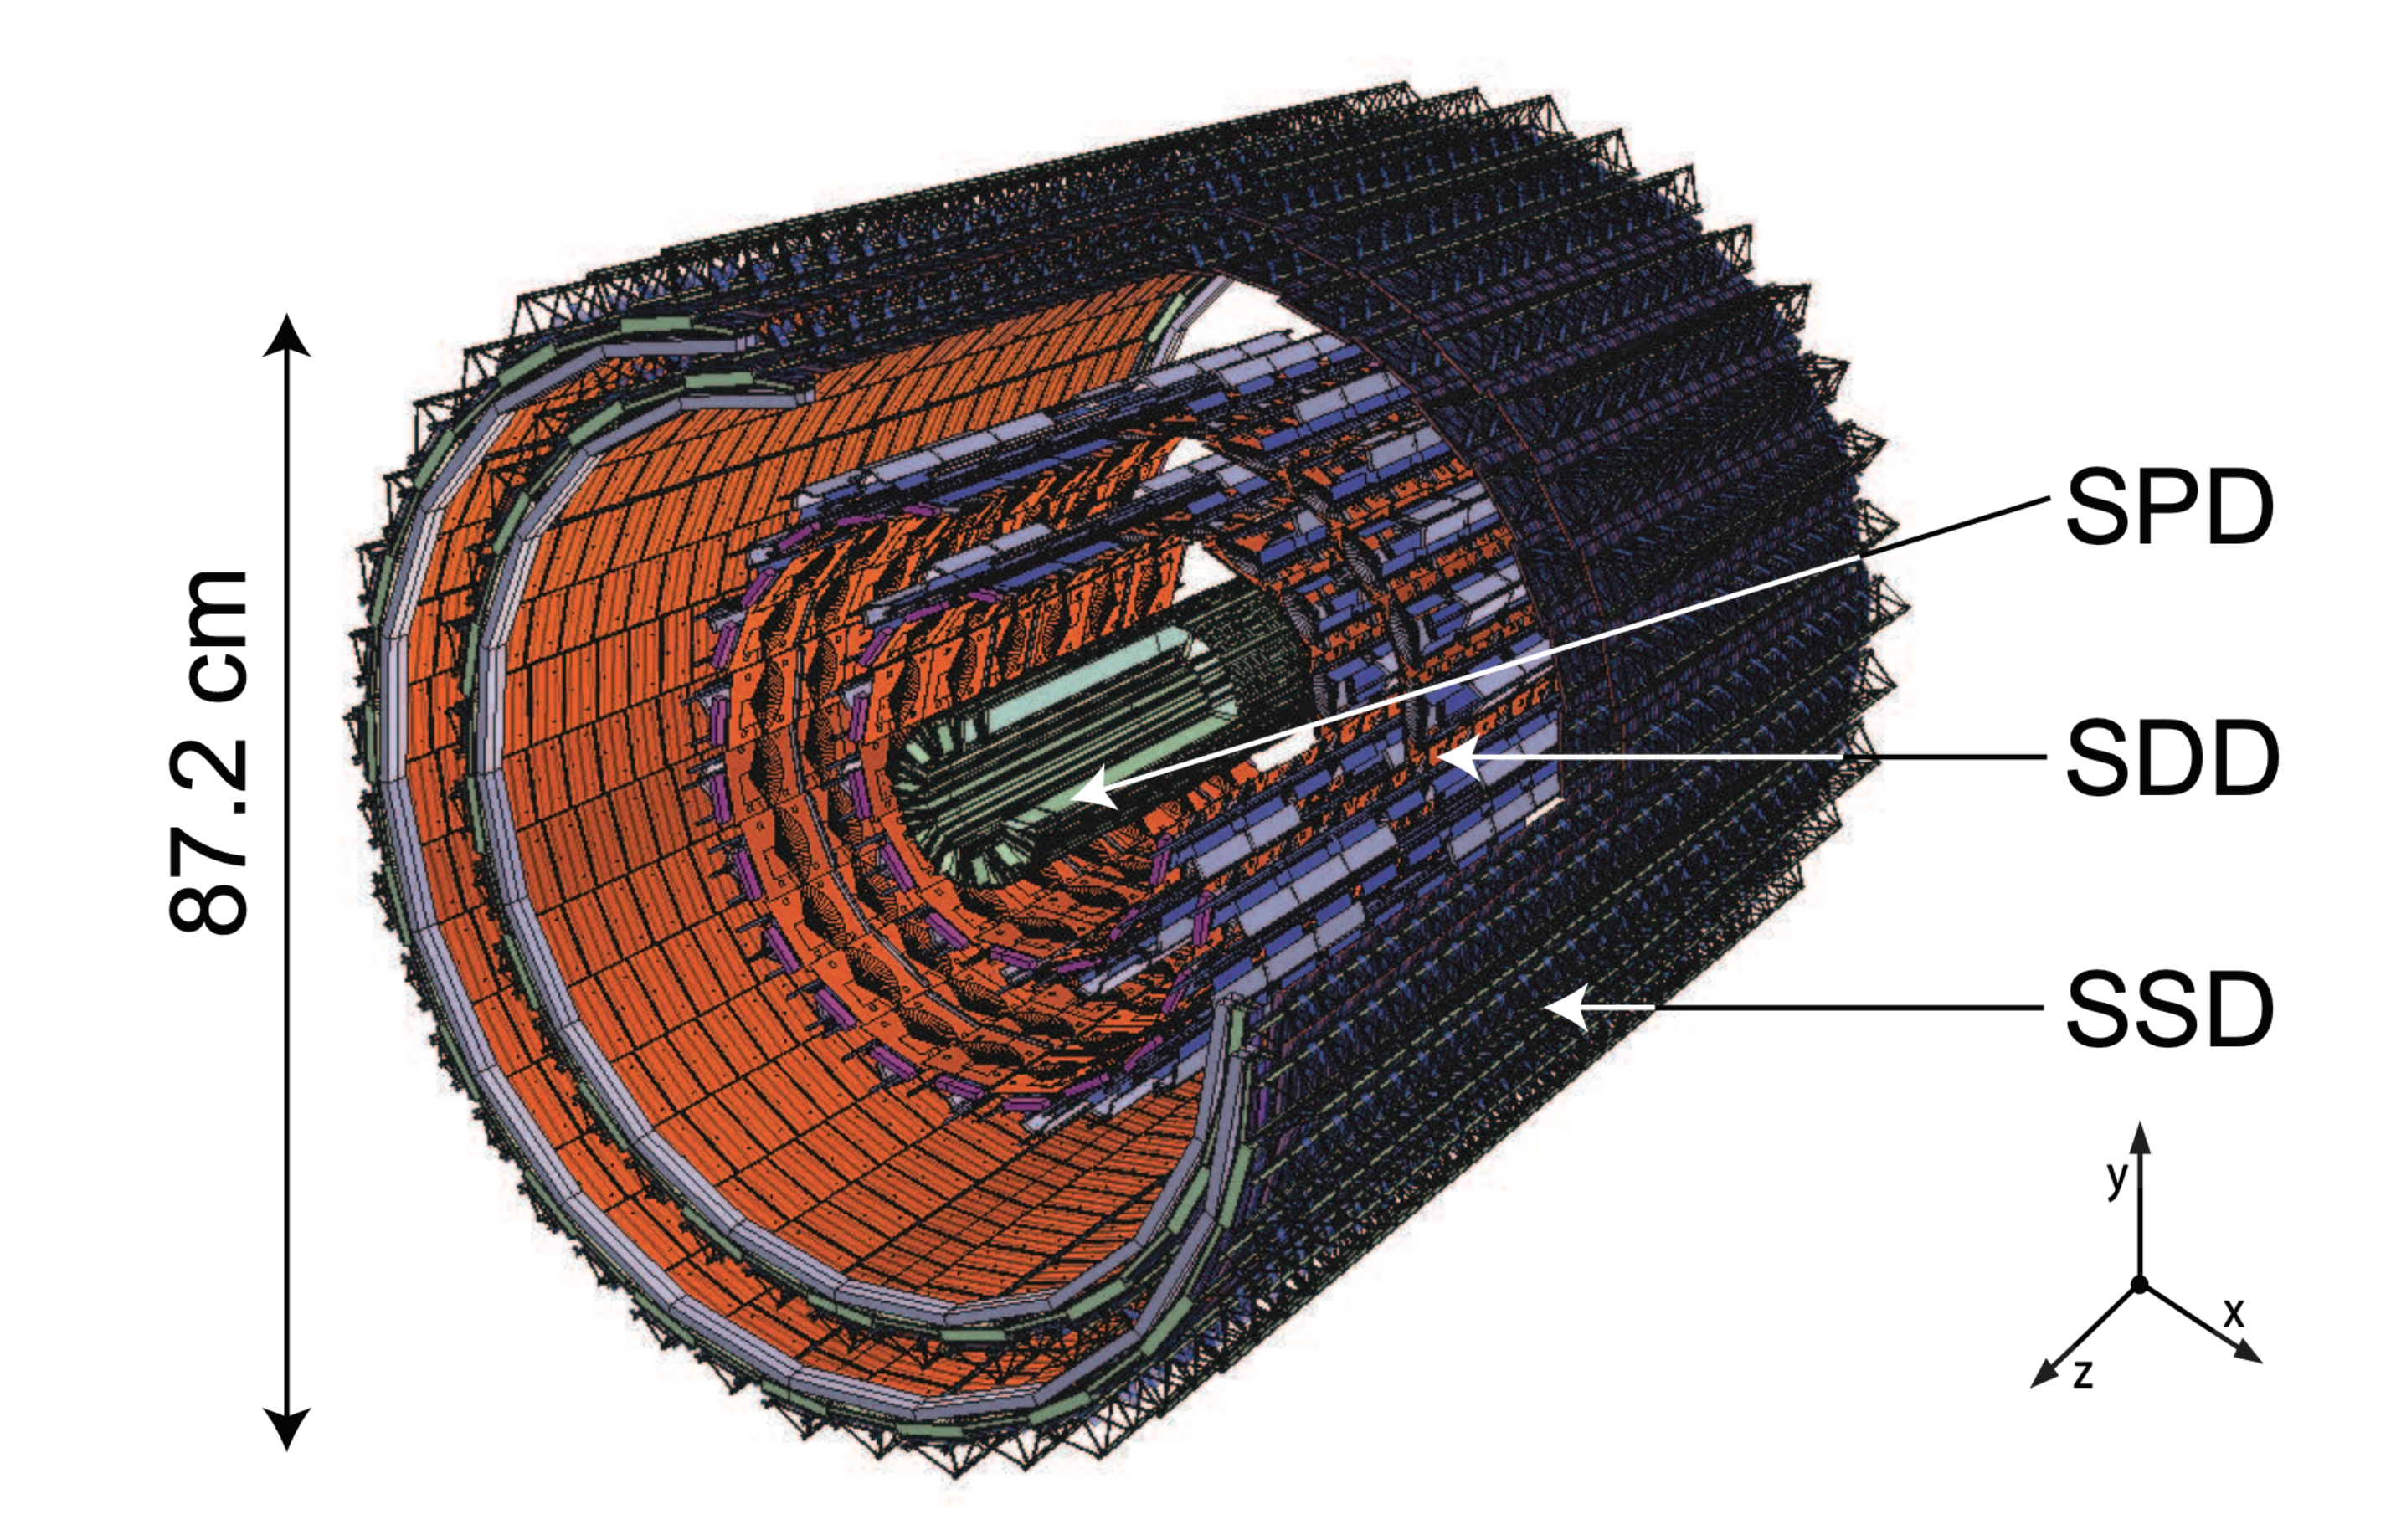
\includegraphics[width=0.8\textwidth]{figures/experiment/its_diagram.png}
    \caption{A schematic of the ITS showing the six layers of silicon detectors, taken from~\cite{ITSDiagram}.}
    \label{fig:its_schematic}
\end{figure}

The ITS uses different types of silicon detectors for each layer, which will be briefly discussed in the following sections.

\subsection{Layers 1 and 2}

The first and second layers of the ITS are composed of \textbf{Silicon Pixel Detectors} (SPD)~\cite{ITSSPD}. The SPD inner and outer barrel layers have radii of 3.9 cm and 7.6 cm, respectively. The pseudorapidity coverage is $|\eta| < 1.95$, the highest of all the ITS detectors. The SPD is segmented into 10 sectors which each cover 36 degrees in azimuth. Each of these sectors contains 12 modules--caled half-staves--which themselves consist of 10 silicon pixel chips. These chips are 13.68 mm $\times$ 15.58 mm in size and contain 8192 pixels each, corresponding to a pixel size of 425 $\mu$m $\times$ 50 $\mu$m. This small pixel size gives rise to a very low occupancy ($<2$\%) for even the most central Pb--Pb collisions.  As the track densities in the innermost layers are very high (up to 100 tracks/cm$^2$ for central Pb--Pb collisions), the SPD has a very high granularity in order to keep the occupancy low. The SPD is also used to generate the L0 trigger signal, which is used to trigger the readout of the TPC and TRD.

\subsection{Layers 3 and 4}
The middle two layers of the ITS are made up of \textbf{Silicon Drift Detectors} (SDD)\cite{ITSSDD}. These layers extend from an inner radius of 14 cm to an outer radius of 24 cm, and cover the pseudorapidity range $|\eta| < 0.9$. There are 260 large area (7.02 $\times$ 7.53 cm$^2$) SSD modules in total, which are split into two drift regions. As an ionizing particle passes through the drift regions, the resulting electrons \textit{drift} into the collection anodes, which are at the ends of the drift regions and are connected to the frontend readout electronics. This separates the SPD and the SDD in a fundamental way--the data from the SDD is analog, and depends very much on how many electrons were ``knocked loose'' during ionization. The SPD, on the other hand, is digital, and only registers a hit (1) if a charged particle passes through the pixel. This analog information can be used to help identify the ionizing particle species using the Bethe-Bloch formula, which will be discussed in more detail in Section~\ref{sec:tpc}. Furthermore, there are MOS charge injectors~\cite{MOSCharge} connected to the cathodes in the drift region, which provide precise timing information to compute the electron drift velocity. This velocity is needed to precisely measure the location of the initial ionizing particle along the direction of the applied electric field. As the track density in the middle layers is lower than in the innermost layers, the SSD has a coarser granularity than the SPD.

\subsection{Layers 5 and 6}
The last two layers of the ITS are \textbf{Silicon Strip Detectors} (SSD)~\cite{ITSSSD}, which have an inner radius of 38 cm and an outer radius of 43 cm. The SSD covers the pseudorapidity range $|\eta| < 0.9$, and is composed of 1698 modules in total. These modules are a 1536-strip double-sided silicon sensor, with each strip connected to the front-end readout electronics. Similar to the SDD, the SSD collects electrons generated when the ionizing particle travels through the silicon--though the drift distance is \textit{much} smaller (300 microns for the SSD vs. 70.2 mm for the SDD). The SSD provides two dimensional measurements of the ionizing particle's position with a 20 micron resolution in the $r\varphi$ direction. The SSD also captures an analog signal, and is therefore used to help identify the ionizing particle species.


\subsection{ITS Upgrade}
During the long shutdown (LS2) from December 2018 to June 2022, the LHC underwent a fairly substantial upgrade to allow for higher beam energies and luminosities. The luminosity increase from Run 2 (before LS2) to Run 3 (after LS2) was substantial, from 12 inverse femtobarns before the shutdown to well over 200 inverse femtobarns after starting up again~\cite{LHCUpgrade}. As such, the ALICE detector needed to undergo quite a few upgrades to keep up with the increased collision rates. In terms of pure hardware upgrades, only three detectors were affected, namely
\begin{itemize}
    \item the Time Projection Chamber (TPC)~\cite{TPCUpgrade},
    \item the Muon Forward Tracker (MFT)~\cite{MFTUpgrade}, and
    \item the ITS~\cite{ITSUpgrade}.
\end{itemize}
The TPC and MFT upgrades will not be summarized in this thesis\footnote{The author of this thesis was intimately involved with the ITS upgrade, and thus would be unable to provide a fair and unbiased description of the TPC and MFT upgrades.}, but some key features of the ITS upgrade will be discussed in the following sections.

\subsubsection{Motivation for the ITS upgrade}
As mentioned previously, the increased collision rates associated with the higher luminosity LHC beam necessitated an upgrade to the ITS. Previously, the readout rate for the ITS was 1 kHz for both pp and Pb--Pb collisions. The upgraded ITS, on the other hand, is able to readout at 100 kHz for Pb--Pb and 200 kHz for pp collisions, drastically increasing the amount of possible data to be taken over the course of Run 3. The upgraded ITS also has a much finer impact parameter resolution than the previous ITS, improving by a factor of 3 in the $r\phi$ coordinate and by a factor of 5 in the $z$ coordinate. This improved resolution is crucial for the ALICE physics program, as it allows for the reconstruction of more secondary vertices--like those from the decay of a B meson; this was previously not possible with the old detector. The tracking efficiency at lower $p_T$ was also improved, thanks to a strong reduction in the material budget (from 1.14\% $X_0$ to 0.35\% $X_0$).


\subsubsection{Hardware overview}
The upgraded ITS consists of seven layers of silicon detectors, as shown in Figure~\ref{fig:its_upgrade_schematic}. There are a total of 192 \textit{staves}--rows of silicon chips--which cover a total area of 10 square meters. Each chip is of the same technology, which will be discussed in more detail in the next section. The first three layers form the Inner Barrel (IB), and contain 48 staves of 27 cm length. The remaining layers are referred to as the Outer Barrel (OB). The OB is further separated into the Middle Layers (MLs) and Outer Layers (OLs), which correspond to the 4-5th and 6-7th layers, respectively. The MLs each have 54 staves of length 84 cm, and the OLs have 90 staves of 150 cm. The grouping of the layers into the IB and OB has ramifications for the hardware testing procedure, which is described in Section~\ref{sec:hardware_testing}.

\begin{figure}
    \centering
    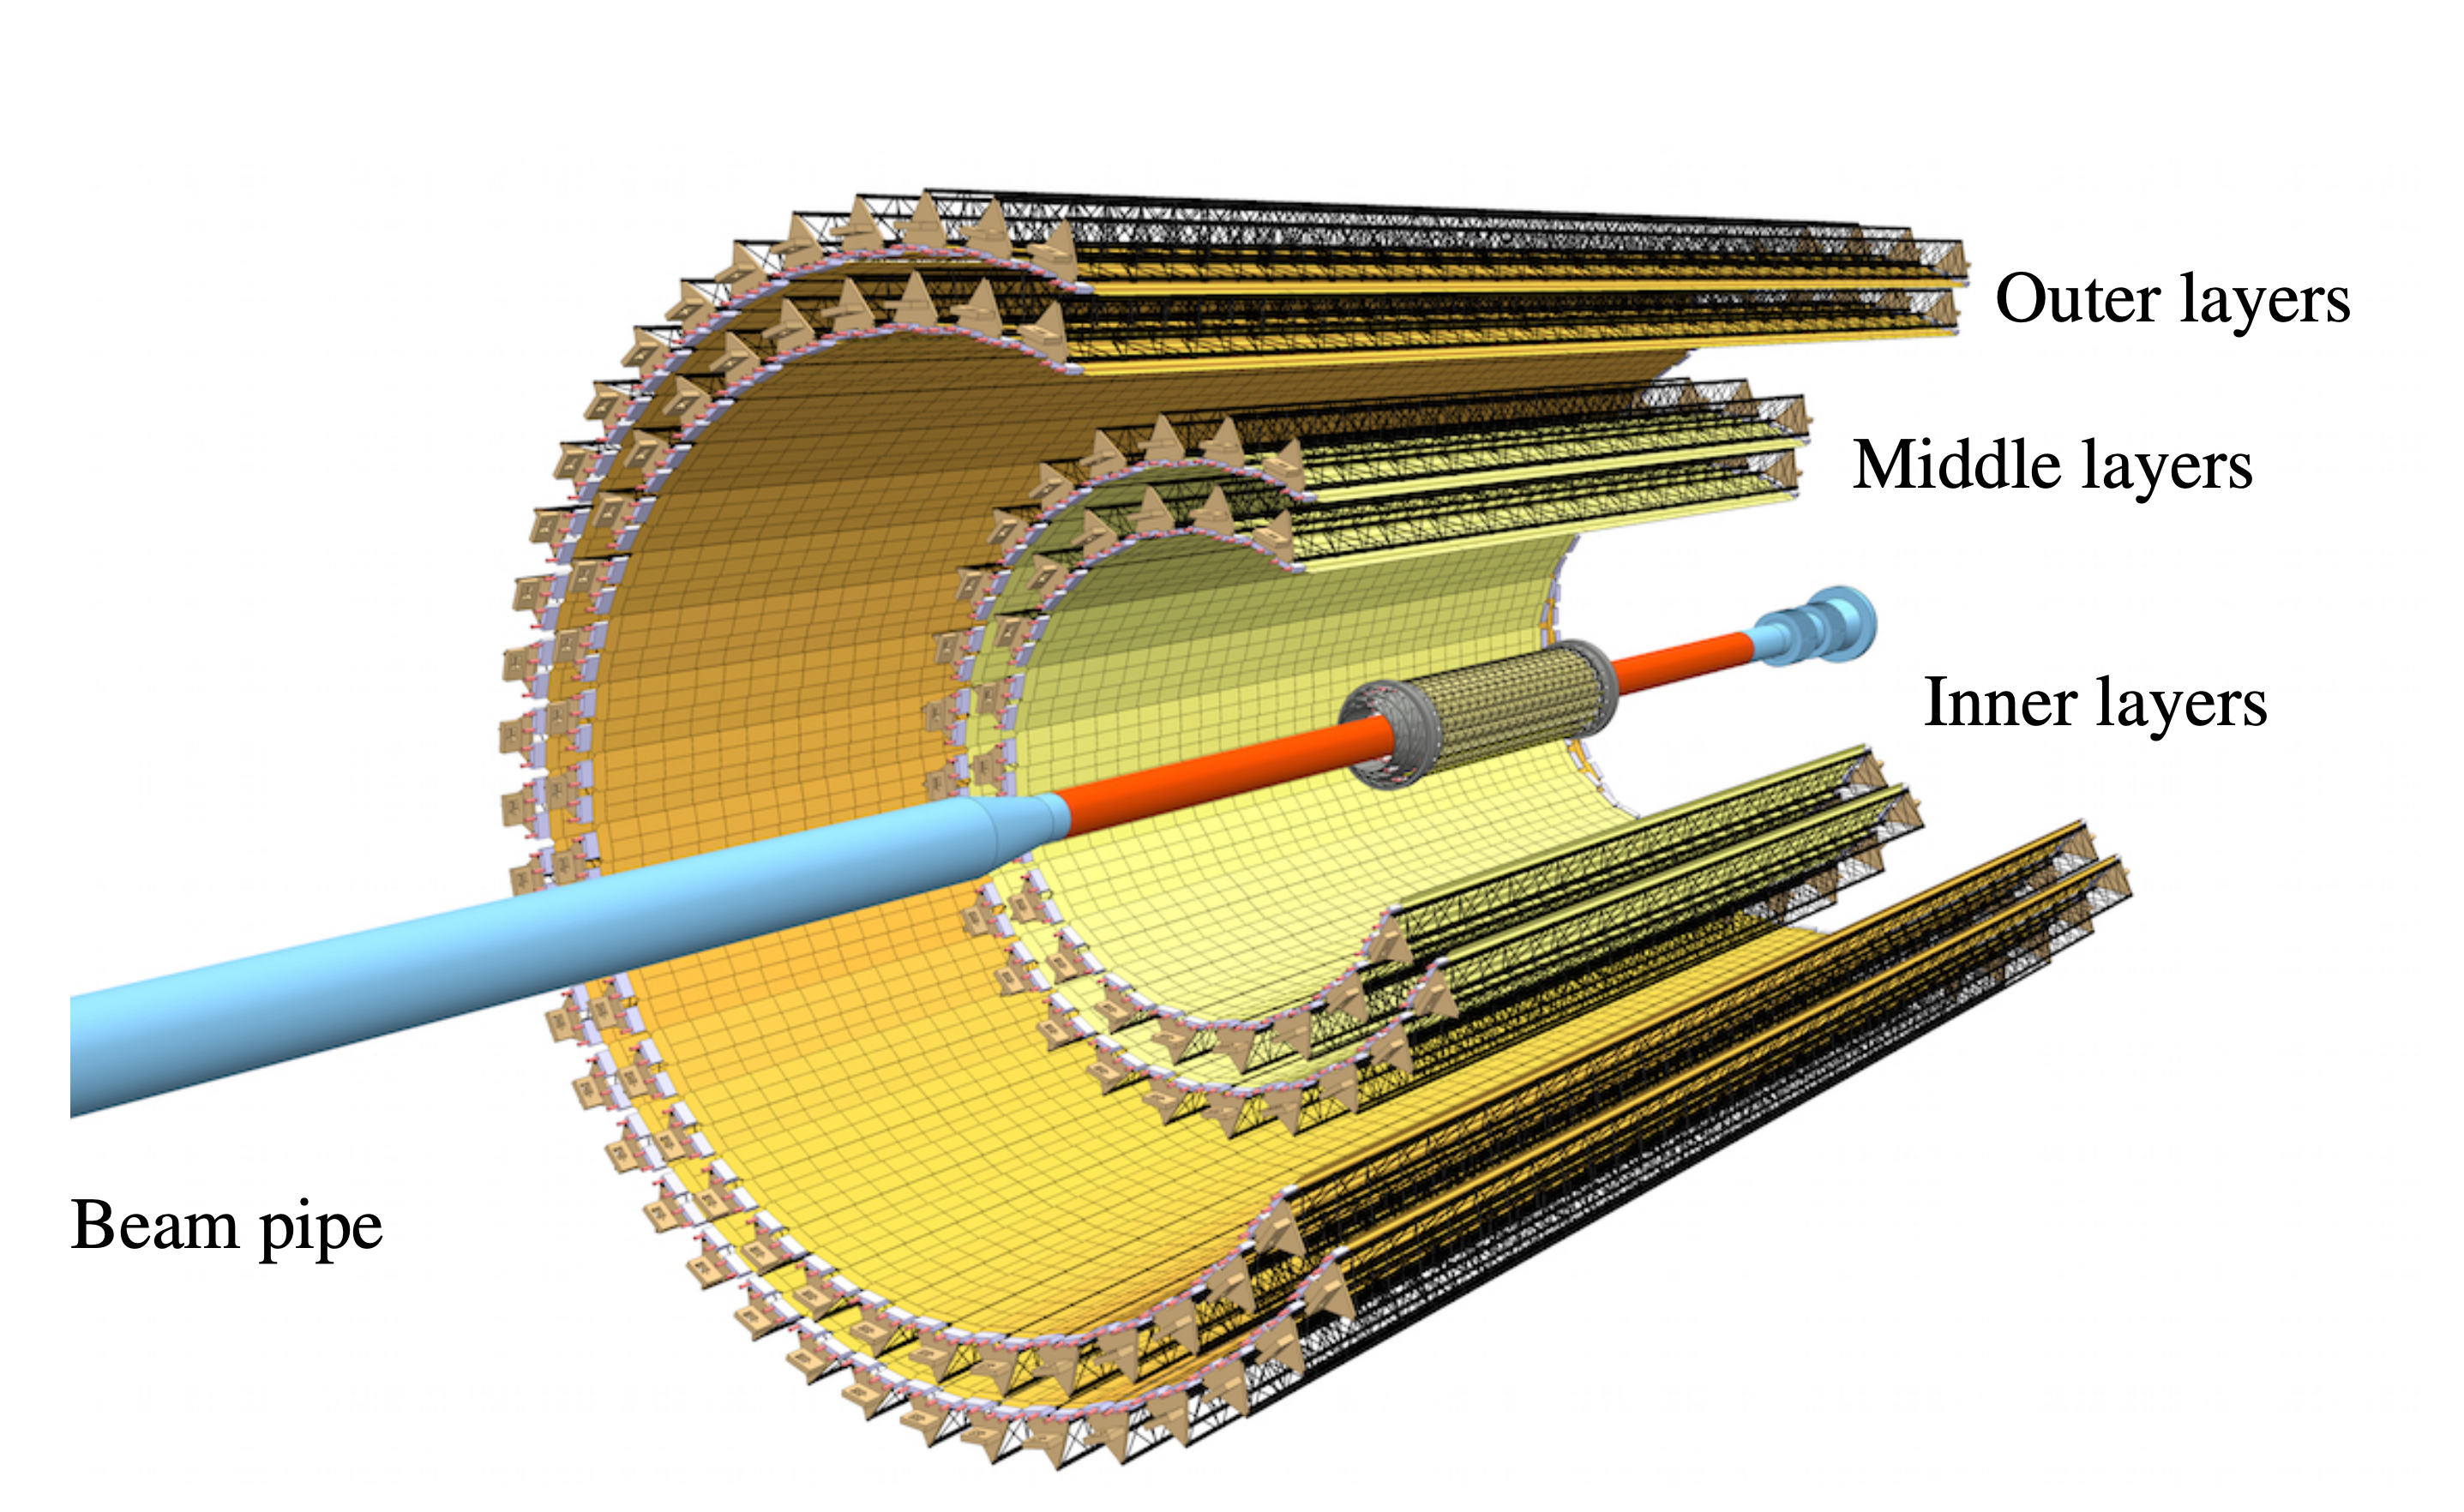
\includegraphics[width=0.8\textwidth]{figures/experiment/its_upgrade_schematic.png}
    \caption{A schematic of the ITS upgrade, showing the seven layers of silicon detectors.}
    \label{fig:its_upgrade_schematic}
\end{figure}


\subsubsection{The ALPIDE chip}
The star of the show for the ITS upgrade is the introduction of a new silicon pixel chip: the ALPIDE~\cite{ALPIDE}. The ALPIDE chip is a CMOS Monolithic Active Pixel Sensor (MAPS) that has a few advantages over its predecessors (e.g. the SPD):
\begin{itemize}
    \item Thanks to a deep p-well, complex logic at the pixel level can be employed. This deeper p-well prevents the n-well PMOS part of the CMOS transistor from collecting unwanted electrons (which are intended for the collection electrodes)
    \item These CMOS transistors allow for complicated in-pixel circuitry, which (when coupled with the priority encoder) \textit{drastically} reduces the data rate by only sending the addresses of ``hit'' pixels to the frontend electronics
\end{itemize}
Each chip is $15\times30$ mm$^2$, and contains over half a million pixels (512 rows, 1024 columns). This corresponds to a spatial resolution of 5 microns, which is much better than the SPD of the old ITS (around 50 microns in $r\varphi$). A diagram of the cross section of an ALPIDE (or more generally a MAPS) pixel can be seen in Figure~\ref{fig:alpide_diagram}. In this diagram, a charged hadron flies through the chip, generating many electron-hole pairs. The electrons are guided to the n-well diode, which ultimately collects the electrons and generates a signal. The CMOS transistors (NMOS and PMOS transistors) are vitally important for the pixel-level logic. Without the deep p-well to protect the PMOS's n-well from wandering electrons, the PMOS (and therefore the CMOS) transistors would be rendered useless.

\begin{figure}
    \centering
    \includegraphics[width=0.8\textwidth]{figures/experiment/alpide_cross.png}
    \caption{A diagram showing the basic operating principle of a MAPS pixel.}
    \label{fig:alpide_diagram}
\end{figure}

These CMOS transistors work together to form the logic within the pixel, shown as a block diagram in Figure ~\ref{fig:alpide_l}. First, the collection diode sends a signal \textit{SUB}, which comes in the form of a large voltage drop in a very short ($\approx 10$ ns) time, followed by a slow requilibration. The \textit{VPULSE} signal is used for testing purposes, where a ``fake'' charge can be sent to the capacitor, generating a similar signal to the collection diode. The resulting \textit{PIX\_IN} signal is sent to an amplifier $+$ signal shaper, and then to a discriminator with threshold \textit{THR}. If the amplified signal is less than the threshold, no \textit{OUT\_D} signal is generated. The digital \textit{OUT\_D} signal is then sent into a simple AND gate, where the other input signal is the digital \textit{STROBE}. This strobing window is ultimately initialized by a trigger signal, and its width is configurable. If the \textit{OUT\_D} signal is high during the strobing window, then one of the three hit storage registers is ``latched'' (i.e. set to one). Also included in the pixel logic is a masking register, which masks the pixel during readout when hot. 

The priority encoder (which physically lies between two columns of pixels) sequentially provides the addresses of the latched pixels to the frontend electronics on the chip. An important feature of the on-pixel electronics and priority encoder is the lack of a clock: this means that there is no activity if there are no hits. In other words, the ALPIDE chip is not sending a bunch of useless 0's to the readout electronics, saving precious bandwidth.

\begin{figure}
    \centering
    \includegraphics[width=1.0\textwidth]{figures/experiment/alpide_logic.png}
    \caption{A block diagram showing the logic embedded on top of a single ALPIDE pixel.}
    \label{fig:alpide_l}
\end{figure}

\subsubsection{Characterizing the chips for commissioning}
\label{sec:hardware_testing}

Each ALPIDE chip has over 500,000 pixels, each with their own circuit logic. Excluding issues with the frontend electronics on the chip, that is still \textit{over} 500,000 possible points of failure. As such, the chips were thoroughly tested to determine if they are worthy of being installed in the ITS. There are three main tests that were performed on each chip:
\begin{enumerate}
    \item \textbf{Fake hit rate}: All pixels are unmasked, and a \textit{STROBE} signal is repeatedly sent to each pixel. As the \textit{THR} signal should prevent any hits from being registered, any latched pixels are considered ``fake hits''.
    \item \textbf{Threshold scan}: A predetermined amount of charge is injected into each pixel via the \textit{VPULSE} signal, and the \textit{THR} signal is varied. There should be a clear threshold where every pixel registers a hit, and vice-versa.
    \item \textbf{Readout tests}: Either a digital signal (by writing the hit storage register) or an analog signal (by injecting charge into the capacitor) pattern is sent to the entire chip, and then the corresponding output is read out. The resulting output should be the same as the input, like the example shown in Figure~\ref{fig:ut_alpide}.
\end{enumerate}

\begin{figure}
    \centering
    \includegraphics[width=0.9\textwidth]{figures/experiment/ut_alpide.png}
    \caption{The signal that was read out from the ALPIDE chip after sending an extremely technical digital input pattern.}
    \label{fig:ut_alpide}
\end{figure}

These tests were run on the ALPIDE software, which is a graphical user interface (GUI) that allows for easy communication with the chips. The resulting output of the tests was simply one of four options, which are summarized in Table~\ref{tab:chip_medals}. This medal system was used to determine where the chip should be installed within the detector. If a chip was GOLD, it was reserved for the IB. If the chip was SILVER, it could be installed in either the MLs or the OLs. If the chip was BRONZE, it could only be installed in the OLs. Finally, if the chip FAILed the tests, it was discarded\footnote{Sent to the poor souls developing the ALPIDE software.}. Further characterization was done at the stave level to determine where within the IB or OB a particular stave should be installed.

\begin{table}
    \centering
    \caption{A summary of the medal system used to determine where a particular chip should be installed. Note that while 99\% \textit{seems} strict, it corresponds to over 5000 misbehaving pixels.}
    \begin{tabular}{|c|c|}
        \hline
        \textbf{Medal} & \textbf{\% of good pixels} \\
        \hline
        GOLD & 99.99\% \\
        SILVER & 99.67\% \\
        BRONZE & 99.00\% \\
        FAIL &  $<$ 99.00\% \\
        \hline
    \end{tabular}
    \label{tab:chip_medals}
\end{table}

\subsubsection{The readout unit}
Another large overhaul for the ITS upgrade was a complete redesign of the readout system, from chip to DAQ. A schematic of the new readout system can be seen in Figure~\ref{fig:its_readout}. Each detector stave is connected to a \textbf{readout unit} (RU) via a relatively long copper data cable. A single RU has a lot of responsibilities, including
\begin{itemize}
    \item communicating with the power board so it can properly power the chips,
    \item receiving the trigger information from the Central Trigger Processor (CTP) and sending it to the chips (which generates the \textit{STROBE} signal discussed above),
    \item receiving \textit{all} of the data from the chips on the stave, which each have their own 1.2 Gbps link (for the IB chips, the OB chips share a 400 Mbps link in groups of seven), and
    \item sending the readout data from the chips to the Common Readout Unit (CRU), 
\end{itemize}
all while being in a highly radiative environment (only 6-8 meters away from the detector). 

\begin{figure}[h]
    \centering
    \includegraphics[width=0.9\textwidth]{figures/experiment/its_readout.png}
    \caption{A schematic of the ITS readout system, showing the various components of the system.}
    \label{fig:its_readout}
\end{figure}

These responsibilities are mostly handled by two on-board field-programmable gate arrays (FPGAs): an SRAM FPGA for actually handling all of the aforementioned data transfer between the various components, and a flash FPGA for ensuring that the SRAM FPGA does not misbehave in the radiative environment. The SRAM FPGA continuously scrubs the flash FPGA to ensure that it has not been misconfigured due to a radiation upset. If it has, the SRAM FPGA will reconfigure it using the ``golden image'' of the SRAM firmware stored in the flash memory of the flash FPGA (hence the name). Even still, the important modules of the SRAM FPGA are triplicated, meaning that if one module is subject to a radiation upset, the other two can outvote it. An image of the RU at the University of Texas at Austin can be seen in Figure~\ref{fig:ut_ru}.

\begin{figure}
    \centering
    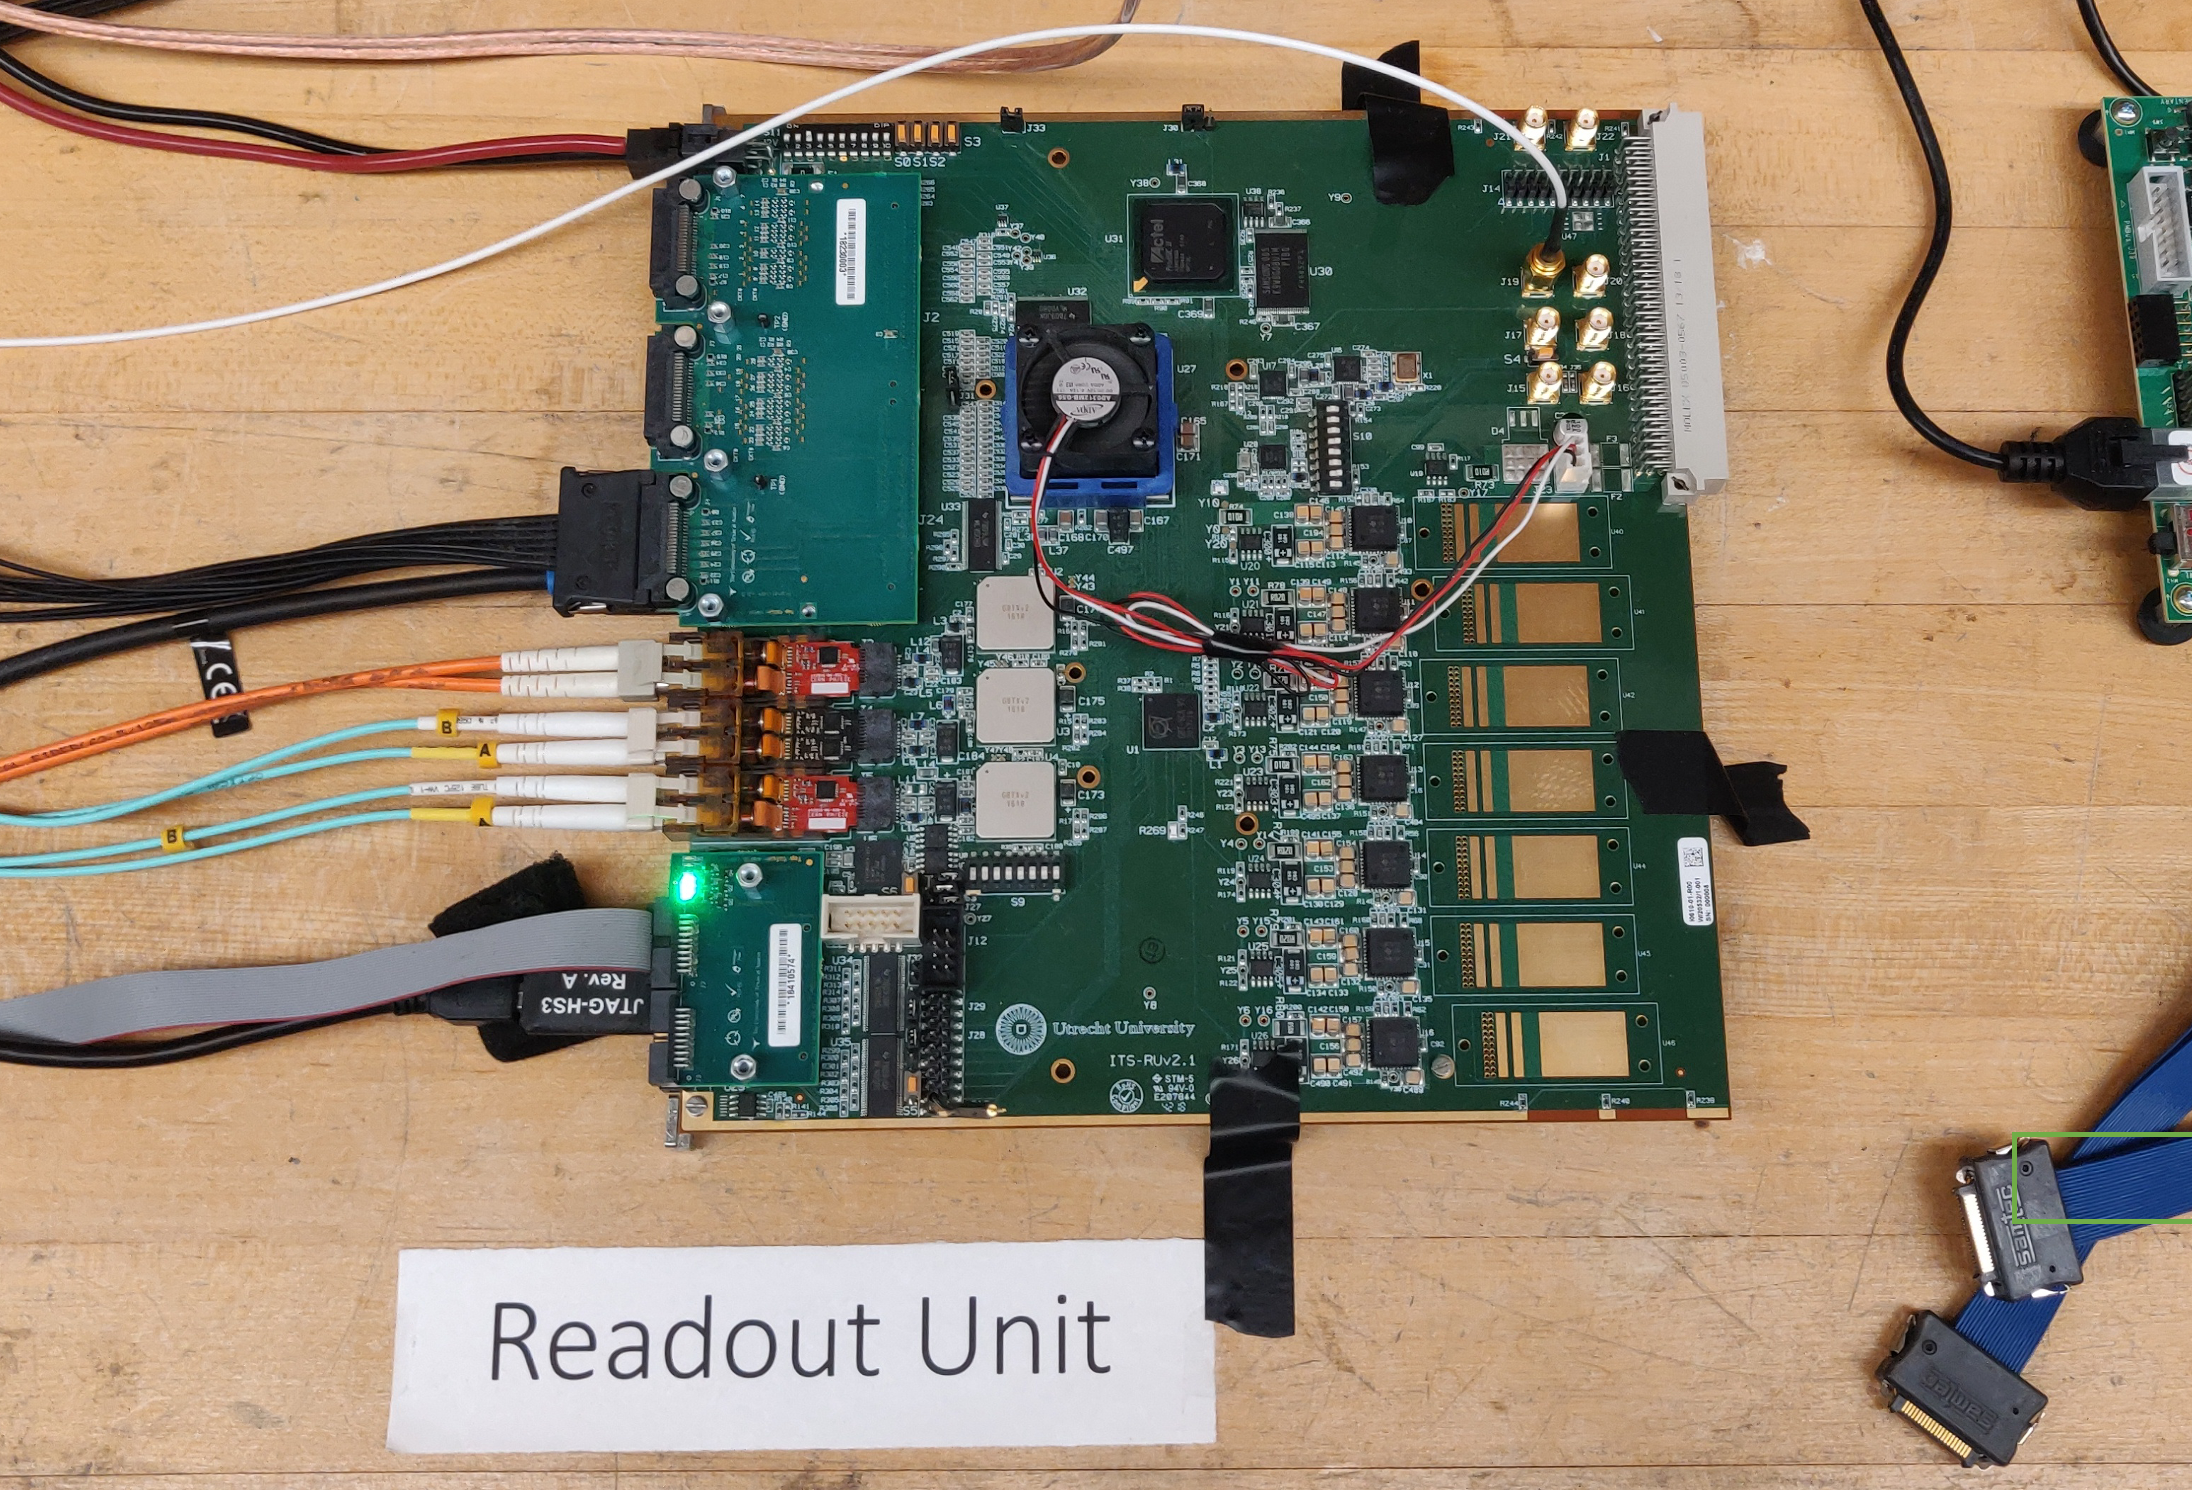
\includegraphics[width=0.9\textwidth]{figures/experiment/ut_ru.png}
    \caption{A picture of a readout unit in its (not-so) natural habitat at the University of Texas at Austin. The heat sink and fan are covering the main SRAM FPGA, and to its north-east is the flash FPGA.}
    \label{fig:ut_ru}
\end{figure}

\section{The Time Projection Chamber}
\label{sec:tpc}
The largest component of the ALICE detector is known as the Time Projection Chamber (TPC)~\cite{TPC1, TPC2}. The TPC is a gas-filled volume with an 85 cm inner radius, a 250 cm outer radius, and a five meter length along the beam axis. This corresponds to an active volume of around 90 cubic meters, all of which is filled with a Ne-CO$_2$-N$_2$ (90-10-5) gas mixture. The TPC has The TPC is an ionizing drift detector: charged particles moving through the detector ionize the gas, and the resulting electrons drift towards the endplates of the detector\footnote{A very similar mechanism to the SDD, on a much larger scale.}--heavily coerced by the presence of a strong 400 V/cm electric field along the z-axis. This electric field is generated by a central cathode that is kept at a potential of 100 kV. A schematic of the TPC field cage can be seen in Figure~\ref{fig:tpc_schematic}.

\begin{figure}
    \centering
    \includegraphics[width=0.9\textwidth]{figures/experiment/tpc_schematic.png}
    \caption{A schematic of the TPC field cage, taken from~\cite{TPC1}}
    \label{fig:tpc_schematic}
\end{figure}

Readout chambers with design based off of the Multi-Wire Proportional Chamber (MWPC) technique are installed at both endplates. In short, these chambers contain an array of wires held at a high voltage are placed in front of a plane of pads held at ground. The electrons that drift towards the endplate pass through this region, which causes a localized cascade of ionization\footnote{Often called a Townsend avalanche, where the ionizing electrons from the initial ionization of the ionizable gas ionize the ionizable gas, creating more ionizing electrons to ionize more ionizable gas...} that is ultimately collected by the pads. The inner readout chamber has 5504 total pads, while the outer readout chamber (i.e. the one actually visible in Figure~\ref{fig:tpc_schematic}) has nearly 10000. The pads are grouped into 18 trapezoidal sectors, each of which covers 20$^\circ$ in azimuth. Unfortunately the boundaries of these sectors don't contain any pads, resulting in very narrow ``dead zones'' within the azimuthal acceptance of the TPC. Using information from both the ITS and TPC, it is possible to reconstruct particle tracks with a resolution of 1 mm in the transverse plane and 2 mm in the longitudinal direction. The momentum resolution in the transverse plane is also very good, staying below 5\% from zero to well over 100 GeV/c.

The TPC is also capable of providing information that can be used to identify particles. As a charged particle travels through the active volume of the TPC, it loses energy as it ionizes the gas in a way that only depends on the particle's velocity. This energy loss is often described by the Bethe-Bloch formula~\cite{BetheBlochPDG}
\begin{equation}
    \left\langle-\frac{d E}{d x}\right\rangle=K z^2 \frac{Z}{A} \frac{1}{\beta^2}\left[\ln \frac{2 m_e c^2 \beta^2 \gamma^2}{I}-\beta^2-\frac{\delta(\beta \gamma)}{2}\right]
\end{equation}
where $K$ is a constant coefficient ($\approx 0.31$ MeV mol$^{-1}$ cm$^2$), $z$ is the charge of the particle, $Z$ and $A$ are the atomic and mass numbers of the gas, $\beta$ is the velocity of the particle in units of the speed of light, $\gamma$ is the Lorentz factor, $m_e$ is the mass of the electron, $c$ is the speed of light, and $I$ is the mean excitation energy of the gas. An important feature of this equation is that most of the parameters depend on the gas mixture and the mass of the electron. For a fixed gas mixture, this equation gives a relationship between the energy (loss) and the velocity of the particle. As the momentum of the particle is known, the mass (and therefore the particle species) can be determined. To see this explicitly, it is useful to look at a common parameterization of the Bethe-Bloch formula~\cite{BetheBlochALEPH},
\begin{equation}
    f(\beta \gamma)=\frac{P_1}{\beta^{P_4}}\left(P_2-\beta^{P_4}-\ln \left(P_3+\frac{1}{(\beta \gamma)^{P_5}}\right)\right),
\end{equation}
where parameters $P_i$ only depend on the gas mixture. Rewriting this equation in terms of the momentum $p$ of the particle gives a curve for each particle species with mass $m_i$,
\begin{equation}
    \label{eq:bethe_bloch_par}
    f(p, m_i)= P_1 \left(\frac{\sqrt{m_i^2 + p^2}}{p}\right)^{P_4} \left(P_2 - \left(\frac{p}{\sqrt{m_i^2 + p^2}}\right)^{P_4}  - \ln \left(P_3 + \frac{m_i^{P_5}}{p^{P_5}} \right) \right).
\end{equation}

\begin{figure}
    \centering
    \includegraphics[width=0.9\textwidth]{figures/experiment/tpc_pid_curves.png}
    \caption{The energy loss signal for different particle species using the ALICE TPC gas mixture, taken from~\cite{BetheBlochALEPH}. The solid lines represent the expected energy loss signal for each particle species (Equation~\ref{eq:bethe_bloch_par}).}
    \label{fig:tpc_pid_curves}
\end{figure}

Examples of the energy loss signal for different particle species using the ALICE TPC gas mixture can be seen in Figure~\ref{fig:tpc_pid_curves}. Note that while there are clearly defined lines for each particle species from Equation~\ref{eq:bethe_bloch_par}, the actual signal is spread out around these lines due to the energy loss and momentum resolution of the TPC. Furthermore, many of the curves intersect at higher momentum. As such, it is useful to define the quantity 
\begin{equation}
n\sigma_{\text{TPC}} = \frac{\langle dE/dx \rangle_{\text{meas}} - \langle dE/dx \rangle_{\text{exp}}}{\sigma_{\text{TPC}}},
\end{equation}
which is the number of standard deviations away from the expected energy loss signal for a given particle species. If an unidentified particle has an $n\sigma_{\text{TPC}}$ value close to zero, it is likely that the particle is of that species. However, when investigating a specific particle species, compromises must be made--requiring a low $n\sigma_{\text{TPC}}$ value may result in less contamination from other particle species, but also yields lower statistics.

\section{The Time of Flight detector}
\label{sec:tof}

The Time of Flight (TOF) detector~\cite{TOF1} is a large array of Multi-gap Resistive Plate Chambers (MRPCs)~\cite{TOF2} that is used to measure the time of flight of charged particles from the nominal interaction point. The TOF is located directly outside of the TPC at a radius of around 3.7 meters, and covers the pseudorapidity range $|\eta| < 0.9$. It consists of 1593 MRPC strips, arranged in 18 sectors along the azimuthal direction. Each MRPC strip has two rows of 48 pickup pads with area 3.5 $\times$ 2.5 cm$^2$, to ensure low occupancy even in the most crowded events. This gives a total of 96 pads per strip and 152928 readout channels in total. The TOF MRPC has a double-stack structure; each of the two stacks has five gas gaps each. The resistive plates are made of standard soda-lime glass sheets. The gap (250 µm) is created by commercial fishing line stretched over the glass sheets. The average MRPC time resolution, including the effects of the full front-end and readout electronics, was measured to be better than 50 ps in a beam test setup.

\begin{figure}
    \centering
    \includegraphics[width=0.9\textwidth]{figures/experiment/tof_pid_curves.png}
    \caption{The time of flight signal $\beta_{\text{TOF}}$ measured in 5.02 TeV Pb--Pb collisions for different particle species as a function of momentum~\cite{TOFPIDPlot}. The curves are labeled with the particle species they correspond to.}
    \label{fig:tof_pid_curves}
\end{figure}

The primary goal of the TOF detector is particle identification: the time of flight of a particle is directly related to its velocity (as the TOF is a fixed length away from the interaction point), which can be used with the particle's momentum to determine its mass. More explicitly, the velocity $\beta$ of a particle is given by (in natural units)
\begin{equation}
    \beta_{\text{TOF}} = \frac{L}{t_{\text{TOF}}},
\end{equation}
where $L$ is the distance from the interaction point to the TOF (3.7 meters) and $t_{\text{TOF}}$ is the time of flight of the particle. Using $p =  m \frac{\beta}{\sqrt{1-\beta^2}}$, $\beta_{\text{TOF}}$ can be written as a function of $p$ for a particle of mass $m_i$,
\begin{equation}
    \beta_{\text{TOF}}(p, m_i) = \frac{p}{\sqrt{p^2 + m_i^2}}.
\end{equation}
Much like the TPC, plotting the TOF signal versus momentum provides a unique curve for each particle species, as shown in Figure~\ref{fig:tof_pid_curves}. Also much like the TPC, the signal is spread out around the expected curve due to the timing resolution of the TOF and momentum resolution of the TPC $+$ ITS. As such, the quantity
\begin{equation}
n\sigma_{\text{TOF}} = \frac{\beta_{\text{meas}} - \beta_{\text{exp}}}{\sigma_{\text{TOF}}},
\end{equation}
is defined, which serves a similar purpose to $n\sigma_{\text{TPC}}$.



\section{The Electromagnetic Calorimeter}

The Electromagnetic Calorimeter (EMCal)~\cite{EMCAL1, EMCAL2} is a sampling calorimeter that consists of lead and polystyrene scintillator layers. The EMCal is made of towers, which are stacks of 76 lead layers (1.44 mm thick) and 77 polystyrene layers (1.76 mm thick). Each tower has a size of about 6.0 $\times$ 6.0 $\times$ 24.6 cm$^3$ and has an individual readout. The towers are arranged into 2 $\times$ 2 groups called modules, which are the smallest units of the detector. The modules are further assembled into larger supermodules (12 $\times$ 24 modules), each weighing about 7.7 metric tons. The EMCal has a total of 10 full-size supermodules and 2 one-third size supermodules, corresponding to 3072 modules and 12,288 towers. It covers a pseudorapidity range of $|\eta| < 0.7$ and an azimuthal angle range of  $\Delta\varphi = 107^\circ$. It is positioned around 4.5 meters from the beam line, between the space-frame support structure and the L3 magnet coils. Schematics of the detector components can be seen in Figure~\ref{fig:emcal_schematic}. While not used in this thesis, the University of Texas at Austin was involved in the commissioning of the EMCal, and thus it is worth mentioning for historical purposes.

\begin{figure}
    \centering
    \includegraphics[width=0.9\textwidth]{figures/experiment/emcal_schematic.png}
    \caption{A schematic of the EMCal~\cite{ERIN123}, along with the module and supermodule structure~\cite{ERIN124}.}
    \label{fig:emcal_schematic}
\end{figure}

\section{The VZERO Detector}

The VZERO detector~\cite{VZERO} consists of two end-cap scintillators: the V0A, located in the forward pseudorapidity region ($2.8 < \eta < 5.1$); and the V0C, located in the backward region ($-3.7 < \eta < -1.7$). While most of the interesting physics lies at midrapidity, these detectors are vital for estimating the collision centrality (as discussed in Section~\ref{sec:collision_centrality}). The VZERO detectors also provide a trigger for the other detectors: whenever a coincident signal occurs in the V0A and V0C, a collision event must have occured between the two detectors. The VZERO system is also used to monitor LHC beam conditions and reject beam-gas and beam-halo events. As the data analyzed in this thesis is from p--Pb collisions, only information from the V0A detector--which faces the lead ion beam--is used for determining the multiplicity percentile of the collision events.
\chapter{Analysis Motivation and Methodology}
\label{ch:analysis_mnm}

This chapter will provide the underlying motivation for the main topic of this thesis, along with a high-level overview of the methodology used to perform the analysis. First, the motivation for this analysis will be given in detail, emphasizing the importance of the \lmb baryon and why it was chosen for this study. Next, the main technique used to perform the analysis will be introduced, along with a brief overview of the analysis procedure. Finally, the main observables of interest will be mathematically defined to avoid any ambiguity in the following chapters.

\section{Motivation}
As mentioned in Section~\ref{sec:strangeness_enhancement}, the enhancement of strange quarks relative to non-strange ($u$ and $d$) quarks in heavy-ion collisions is a key indicator of the production of a QGP. Experimentally, this enhancement is seen by measuring the production of strange hadrons ($\Lambda$, $K^0$, $\phi$, $\Xi$, $\Omega$) relative to the production of pions as a function of event multiplicity. The results of such measurements from the ALICE collaboration is shown again in Figure \ref{fig:ref_enhancement} for reference. 

\begin{figure}
\centering
\includegraphics[width=\textwidth]{figures/introduction/strangeness_enhancement.png}
\caption{The enhancement of strange hadrons relative to pions as a function of event multiplicity in pp, \pPb, and \PbPb collisions at ALICE, taken from \cite{NATURE}.}
\label{fig:ref_enhancement}
\end{figure}

This figure shows a clear indication of an \textit{onset} of strangeness enhancement, which transitions smoothly from low multiplicity pp to high multiplicity Pb--Pb in a way that is independent of collision system. While statistical models are able to well-describe these particle ratios in low multiplicity pp (in the form of the canonical SHM from Section~\ref{sec:shm} without chemical equilibriation~\cite{NATURE14, NATURE15}) and high multiplicity Pb--Pb (with the grand canonical SHM and full chemical equilibriation~\cite{NATURE12, NATURE13}), such models cannot describe the transition region. Phenomenological extensions to these models are able to produce a smooth transition between the two regimes~\cite{NATURE16, NATURE17}, but the microscopic origins of this observed enhancement are still unknown. 

This thesis aims to shed light on these origins by investigating this enhancement in different kinematic regimes. In particular, the production of strangeness within the near-side and away-side components of dijets\footnote{For more details see Section~\ref{sec:jet_quenching} in the introduction.} will be studied and compared with the strangeness production outside of the dijet system. The production in the near-side component of the dijet corresponds to mostly unmodified strange quark production in a jet, whereas the away-side production corresponds to strangeness production in a jet whose initial partons traversed through the QGP medium. The production outside of the dijet system is meant to represent the production of strangeness in the QGP medium itself, and serves as a baseline for ``soft'' quark production. Measuring the strangeness production in these regions can be used to determine their relative contributions to the overall observed enhancement, in turn illuminating some of its origins at a fundamental level.

The p--Pb collision system is ideal for this study for two major reasons. The first is that the p--Pb system captures the \textit{entirety} of the observed onset of strangeness enhancement, as seen in Figure~\ref{fig:ref_enhancement}. Thus, when trying to study this onset, \pPb collisions are the most natural choice. The second reason is that pp collisions give rise to a large amount of jet-like production, with very little medium-like production. Pb--Pb collisions, on the other hand, are dominated by medium-like production with very little jet-like contributions. The p--Pb system produces a significant amount of both jet- and medium-like production, making it the ideal candidate for analyzing the production of strangeness in these two regimes.

\subsection{The \lmb baryon}
\label{sec:lambda_baryon}

When studying strange quark production in experiment, a choice of strange hadron must be made. In this thesis, the strange hadron of choice is the \textbf{lambda baryon} (\lmb). The \lmb is a neutral hadron with mass $1.116$ \GeVmass, consisting of one up, one down, and one strange quark ($uds$). The reasons for choosing the \lmb baryon for this analysis are as follows.

Firstly, it is the lightest baryon containing a strange quark, and is thus the most abundantly produced strange baryon in high energy particle collisions. This makes it an ideal candidate for differential studies--like the one presented in this thesis--as correlation measurements require a significant sample size to extract statistically meaningful trends. Second, the \lmb has a very long lifetime--relative to the collision evolution--as it can only decay weakly. This has two effects:
\begin{enumerate}
    \item \lmb baryons produced early on in the collision survive until the end of the collision, keeping their decay products in-tact. This is not the case for strongly decaying resonace states like the $K^*$, which often decay within the hadronic gas phase of the collision. This can result in their decay products ``rescattering'' off other hadrons within the gas~\cite{Rescatter}, making it impossible to reconstruct the original resonance.
    \item The \lmb often travels a significant distance before decaying, which allows for the reconstruction of its decay vertex in the detector. This substantially reduces the background contribution to the \lmb signal, which is discussed in more detail in Section~\ref{sec:v0_decay}
\end{enumerate}
Furthermore, the integrated production of \lmb baryons relative to pions has been studied extensively in pp, p--Pb and Pb--Pb collisions at ALICE, as shown in Figure~\ref{fig:lambda_enhancement}. Due to its strange quark content, the \lmb/pion ratio exhibits a large enhancement, especially in the p--Pb region. The measurements in Figure~\ref{fig:lambda_enhancement} serve as a baseline for the differential studies presented in this thesis.

\begin{figure}
\centering
\includegraphics[width=\textwidth]{figures/mnm/lambda_enhancement.png}
\caption{The \pt-integrated \lmb/pion ratio as a function of event multiplicity in pp, p--Pb, and Pb--Pb collisions at ALICE.}
\label{fig:lambda_enhancement}
\end{figure}

Finally, the \lmb baryon, with a net strangeness of one, shares a similar mass with the $\phi(1020)$ resonance ($s\bar{s}$), which has a net strangeness of zero. Thus the differences between ``open'' strangeness ($|S| > 0$) and ``hidden'' strangeness ($|S| = 0$) can be studied by comparing the production of \lmb baryons with the production of $\phi$ resonances. Due to their similar masses, any changes in the production of these two hadrons due to differing masses would be negligible.

\section{Methodology}

\subsection{The main technique}
To separate the production of \lmb baryons into the jet and non-jet regions, \textbf{two-particle angular correlations} are used. By looking at the relative azimuthal angles $\Delta\varphi = \varphi_{\text{trigger}} - \varphi_{\text{associated}}$ between a high momentum \textbf{trigger} particle and a lower momentum \textbf{associated} particle, the resulting distribution can be used to separate the production of the associated particles into distinct regions. These regions can be seen in Figure~\ref{fig:dphi_cartoon}, and will be referred to as
%
\begin{itemize}
\item the \textbf{near-side region} shown in red, corresponding to near-side jet production with no medium interactions, 
\item the \textbf{away-side region} shown in blue, corresponding to away-side jet production with possible medium interaction, and
\item the \textbf{underlying event (UE) region} shown in green, corresponding to the production within the medium that is not correlated with a jet.
\end{itemize}
%
\begin{figure}
\centering
\includegraphics[width=\textwidth]{figures/mnm/dphi_cartoon.png}
\caption{A cartoon of a Pb--Pb (p--Pb) collision that produces particles in the near- and away-side jets, along with the UE. The corresponding regions in the $\Delta\varphi$ distribution are highlighted on the right.}
\label{fig:dphi_cartoon}
\end{figure}

The clear separation between these regions in the $\Delta\varphi$ distribution can be understood from the following argument. If the trigger momentum is high enough ( $>$ 4 GeV/$c$), it must be closely aligned with the near-side jet axis~\cite{JetAxisArgument}. As such, the associated particles that are produced in the near-side of the jet will have a small relative angle to the trigger, near $\Delta\varphi = 0$. The associated particle production in the away-side jet would then be 180$^\circ$ away from the trigger, near $\Delta\varphi = \pi$. Finally, the uncorrelated\footnote{Elliptic flow ($v_2$) gives rise to a small correlation across $\Delta\varphi$, see Section~\ref{sec:collective_flow}.} associated particle production within the medium would be randomly distributed across $\Delta\varphi$, manifesting as a (mostly) flat background that the near- and away-side peaks sit on top of. 

\subsection{The end goal}

In this thesis, the h-\lmb $\Delta\varphi$ distributions in p--Pb collisions at the ALICE detector will be measured across a wide range of multiplicities. The resulting distributions will be used to extract the associated \lmb yields in each of the near-side, away-side and UE regions. Moreover, the correlation distributions will be used to extract the widths of the near- and away-side jet peaks, which aid in the study of the effects of jet-medium interactions on the production of strange hadrons~\cite{HFWidthPaper}. Each of these observables will be compared with those of a h-h (dihadron) sample, which serves as a proxy for non-strange quark (pion) production. These measurements will be compared with theoretical model predictions from the event generators detailed in Section~\ref{sec:models}. The differences between open and hidden strangeness production will also be explored using previously published h-$\phi(1020)$ angular correlation measurements in \pPb collisions~\cite{JustinPaper}. 

Because the analysis procedure is dense with technical details, the remainder of this chapter will be dedicated to providing a high-level overview of the analysis. The specifics of the analysis procedure will be discussed in Chapter~\ref{ch:analysis_details}.

\subsection{A brief overview of the analysis}
\label{sec:analysis}

To get to the final h-\lmb and h-h $\Delta\varphi$ distributions of interest, a correlation function must be specified. There are a multitude of ways to define such correlation functions~\cite{CorrelationFunction}, but this thesis uses the per-trigger normalized associated particle yield,
\begin{equation}
    C_{\text{yield}}(\Delta\varphi, \Delta\eta) = \frac{1}{N_{\text{trig}}}\frac{d^2N_{\text{pair}}}{d\Delta\varphi d\Delta\eta}.
\label{eq:corr}
\end{equation}
Note that this is a 2D distribution, which has information about the angular separation in both $\Delta\varphi$ \textit{and} $\Delta\eta$. Due to the finite acceptance of the detector along $\eta$, na\"ively integrating over $\Delta\eta$ (in other words, just looking at the angular separation in $\Delta\varphi$) would introduce a bias in the jet components, which will be discussed in Section~\ref{sec:acceptance_corr}. As mentioned previously, the angular separations $\Delta\varphi$ and $\Delta\eta$ are measured between a high momentum trigger hadron (h)--which serves as a proxy for the jet axis--and a lower momentum associated hadron ($\Lambda$ or h). 

\subsubsection{Raw distribution corrections}
\label{sec:raw_corr}
The correlation function given by Equation~\ref{eq:corr} cannot be directly obtained in data. Instead, a series of corrections to the raw distribution must be applied to correct for various detector inefficiencies and acceptance effects. The \textbf{raw distribution} is defined as the distribution obtained by counting the number of observed trigger-associated pairs within a given event, summed up over the entire event sample. The corrected distribution is then given by
%
\begin{equation}
    C_{\text{yield}}(\Delta\varphi, \Delta\eta) = \frac{1}{N_{\text{trig}}^{\text{corr}}}\frac{1}{\epsilon_{\text{trig}}\times\epsilon_{\text{assoc}}}B(0,0)\frac{S(\Delta\varphi, \Delta\eta)}{B(\Delta\varphi, \Delta\eta)}\frac{1}{\epsilon_{\text{pair}}(\Delta\varphi, \Delta\eta)},
\label{eq:corr_detector}
\end{equation}
%
where $S(\Delta\varphi, \Delta\eta)$ is the aforementioned raw distribution. $N_{\text{trig}}$ is the total number of trigger hadrons across the event sample, corrected for trigger efficiency. Each of $\epsilon_{\text{trig}}$, $\epsilon_{\text{assoc}}$ and $\epsilon_{pair}$ are efficiency correction factors that are discussed in more detail within Section~\ref{sec:single_particle_corr}.  $B(\Delta\varphi, \Delta\eta)$ is the distribution generated by combining trigger and associated particles that are produced in \textit{separate} events, called the ``mixed-event'' distribution. A simple diagram showing the differences between the generation of $S(\Delta\varphi, \Delta\eta)$ and $B(\Delta\varphi, \Delta\eta)$ is shown in Figure~\ref{fig:mixed_event_cartoon}. This distribution is used to correct for the finite acceptance of the detector, and is detailed in Section~\ref{sec:acceptance_corr}.

\begin{figure}
\centering
\includegraphics[width=\textwidth]{figures/mnm/mixed_event_cartoon.png}
\caption{A simple diagram showing the differences between the generation of the raw distribution $S(\Delta\varphi, \Delta\eta)$ (left) and the mixed-event distribution $B(\Delta\varphi, \Delta\eta)$ (right). The yellow tracks are those observed by the detector. The raw distribution is obtained by looking at trigger-associated pairs within the same event, whereas the mixed-event distribution is generated from pairs that come from separate events. Note that both $\Delta\varphi$ and $\Delta\eta$ cannot be easily shown on a 2D plot, but the distributions are filled with both quantities.}
\label{fig:mixed_event_cartoon}
\end{figure}

Examples of $S(\Delta\varphi, \Delta\eta)$, $B(\Delta\varphi, \Delta\eta)$ and $C_{\text{yield}}(\Delta\varphi, \Delta\eta)$ for h-\lmb pairs can be found in Figure ~\ref{fig:twod_cor}. The peaks observed around $\Delta\varphi = 0$ and $\Delta\varphi = \pi$ in the fully corrected correlation function define the aforementioned near- and away-side regions, respectively, which lie on top of the uncorrelated UE.

\begin{figure}[t]
\makebox[\linewidth][c]{%
\centering
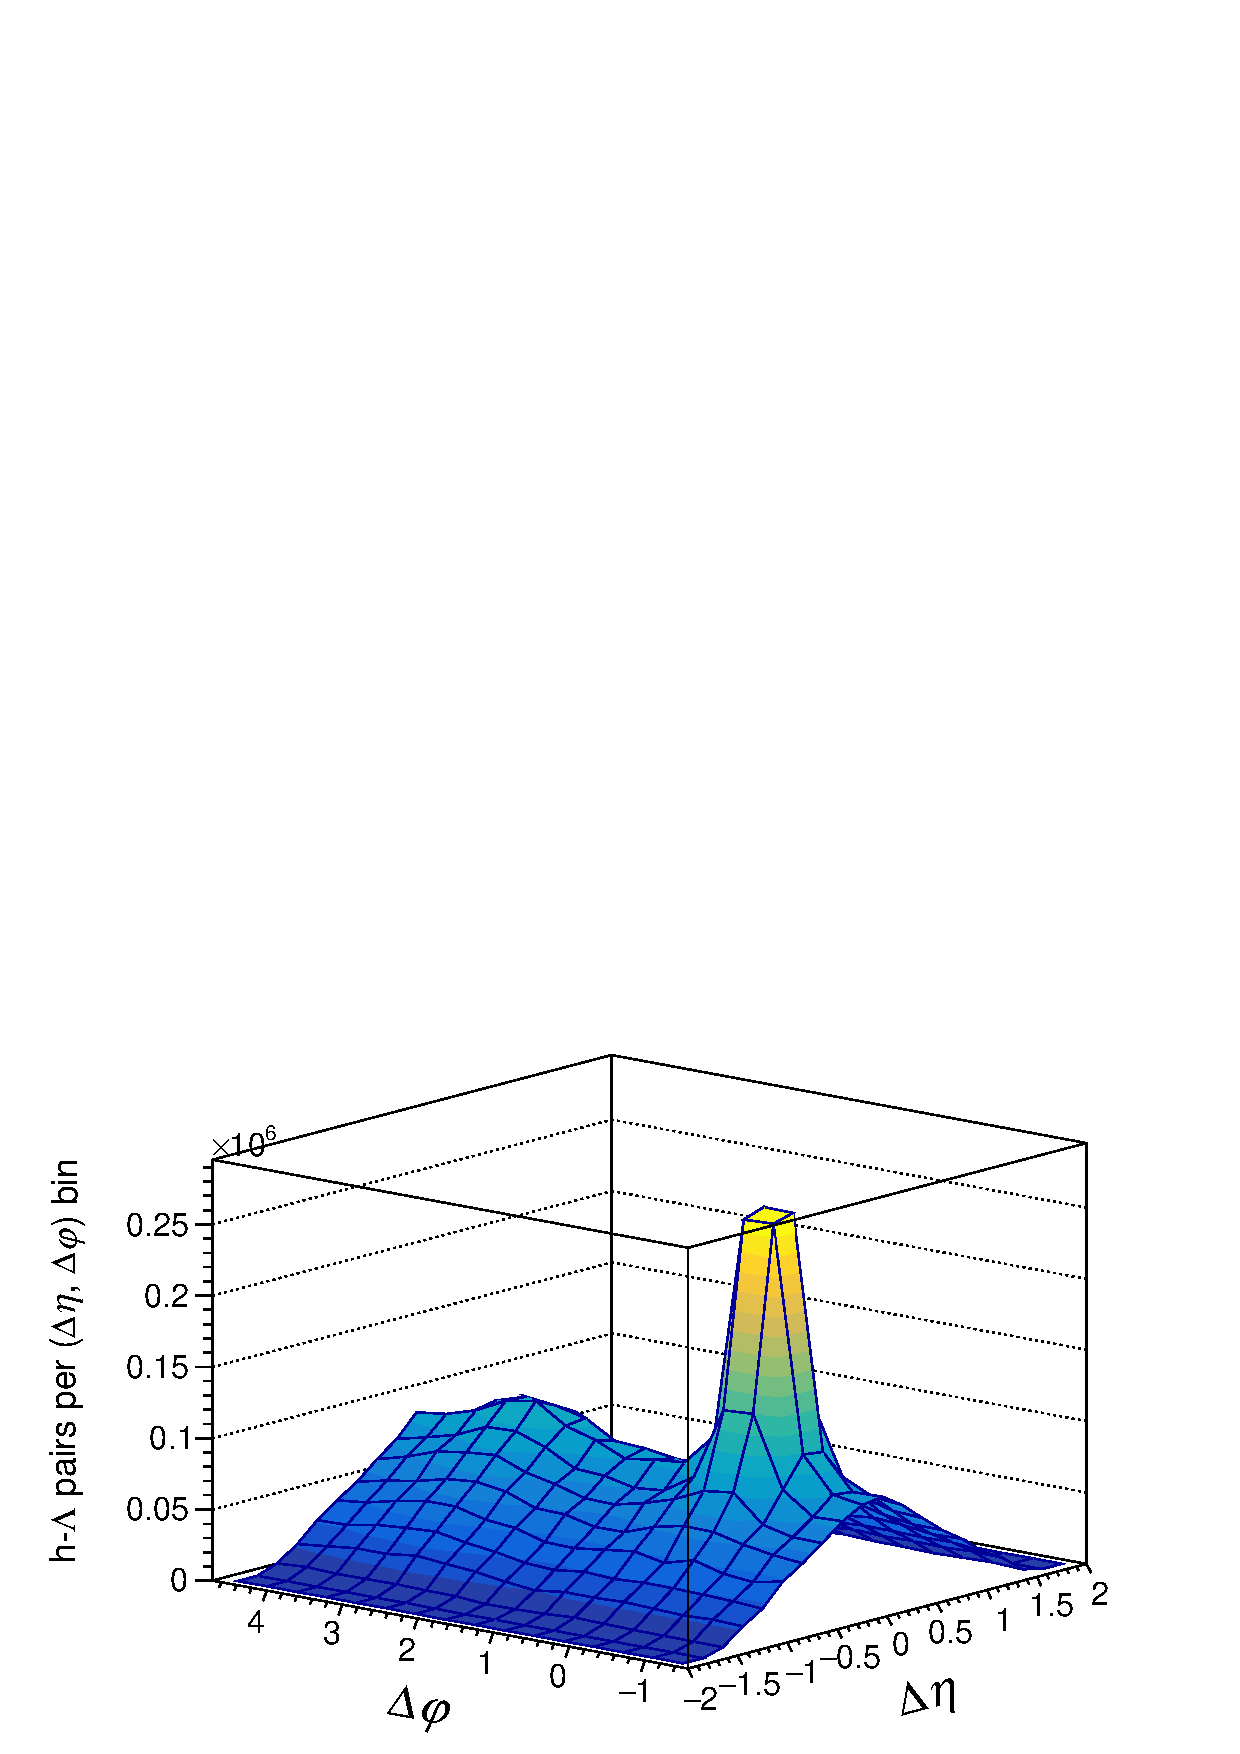
\includegraphics[width=0.35\textwidth]{figures/mnm/h_lambda_2d_nomixcor_20_50_highpt.pdf}
\includegraphics[width=0.35\textwidth]{figures/mnm/h_lambda_2d_mixed_20_50_highpt.pdf}
\includegraphics[width=0.35\textwidth]{figures/mnm/h_lambda_2d_mixcor_20_50_highpt.pdf}
}
\caption{Examples of the h-\lmb same-event distribution $S(\Delta\varphi, \Delta\eta)$ (left), mixed-event distribution $B(\Delta\varphi, \Delta\eta)$ (middle), and fully corrected correlation function $C_{\text{yield}}(\Delta\varphi, \Delta\eta)$ (right).}
\label{fig:twod_cor}
\end{figure}

\clearpage

\subsubsection{Underlying event fit}
\label{sec:uefit}

Once all of the corrections have been applied to the raw distributions, the resulting correlation function $C_{\text{yield}}(\Delta\varphi, \Delta\eta)$ can be projected onto $\Delta\varphi$ to obtain the 1D distribution $dN/d\Delta\varphi$. To extract the near- and away-side widths and the per-trigger yields in each kinematic region from these distributions, the underlying event contribution $U(\Delta\varphi$) must be quantified. While there are multiple ways to do this, the nominal procedure is simply to fix $U(\Delta\varphi)$ to the average of the $\Delta\varphi$ distribution in the regions where there is little-to-no jet contribution. Explicitly, these regions are 
\begin{itemize}
\item $(-\frac{\pi}{2}, -\frac{\pi}{4})$, 
\item $(\frac{\pi}{4}, \frac{5\pi}{8})$, and
\item $(\frac{11\pi}{8}, \frac{3\pi}{2})$. 
\end{itemize}
The effects of varying these regions, along with other assumptions of the form of $U(\Delta\varphi)$, are explored within Chapter~\ref{ch:systematics}.

\subsubsection{Yield and width extraction}
\label{sec:yield_extraction}
 After obtaining the underlying event fit $U(\Delta\varphi)$, the associated particle yields in the jet-like and UE regions are extracted using
 %
\begin{eqnarray}
    Y_{\text{near}} = \int_{-\pi/2}^{\pi/2} (\frac{dN}{d\Delta\varphi}- U(\Delta\varphi))d\Delta\varphi,  \  \ Y_{\text{away}} = & \int_{\pi/2}^{3\pi/2} (\frac{dN}{d\Delta\varphi}- U(\Delta\varphi))d\Delta\varphi 
    \label{eq:jet_yields}
    \\ 
    Y_{\text{UE}} = \int_{-\pi/2}^{3\pi/2} U(\Delta\varphi)d\Delta\varphi,
\label{eq:ue_yield}
\end{eqnarray}
%
where the subscripts near, away and UE refer to the near-side, away-side, and underlying event regions, respectively.

In order to quantify the widths of the near- and away-side peak regions, the $\Delta\varphi$ distributions are fit using the function
%
\begin{equation}
    F(\Delta\varphi) = U(\Delta\varphi) + \frac{e^{\kappa_{\text{near}}\text{cos}(\Delta\varphi - \mu_{\text{near}})}}{2\pi I_0(\kappa_{\text{near}})} + \frac{e^{\kappa_{\text{away}}\text{cos}(\Delta\varphi - \mu_{\text{away}})}}{2\pi I_0(\kappa_{\text{away}})},
\label{eq:fullfit}
\end{equation}
%
which is composed of two von Mises functions describing the near- and away-side peaks. Von Mises functions~\cite{VonMises1, HFWidthPaper} are the circular analogs of Gaussian distributions and provide the best fit to the $2\pi$-periodic $\Delta\varphi$ distributions. The $\kappa_{\text{near}}$ and $\kappa_{\text{away}}$ terms are the measure of the collimation of the near- and away-side peaks, respectively, and $I_{0}$ is the zeroth-order modified Bessel function. The parameters of the underlying event term $U(\Delta\varphi)$ are fixed to those obtained following the procedure in the previous section while fitting the full correlation function. Due to symmetry considerations, the means $\mu_{\text{near}}$ and  $\mu_{\text{away}}$ are also fixed to $0$ and  $\pi$, respectively. The width of the peaks is then quantified via~\cite{VonMises1}
%
\begin{equation}
    \sigma_{\text{near,away}} = \sqrt{-2\log\frac{I_1(\kappa_{\text{near,away}})}{I_0(\kappa_{\text{near,away}})}},
\label{eq:width}
\end{equation}
%
where $I_1$ is the first-order modified Bessel function and $\log(x)$ is the natural logarithm of $x$. As before, the effects of different choices for $F(\Delta\varphi)$ will be detailed in Chapter~\ref{ch:systematics}.
\chapter{Analysis Details}
\label{ch:analysis_details}

This chapter builds upon the analysis overview presented in the previous chapter by providing a much more detailed description of each component of the analysis. These components can be summarized as follows. First, a high-quality data sample of \pPb collisions is selected, with events further differentiated by their multiplicity. Then, quality tracks are selected for the trigger and associated charged hadrons, and the $\Lambda$ baryons are reconstructed from lower quality tracks using their characteristic decay topology. These $\Lambda$ daughter tracks are identified as protons or pions using information from the TPC and TOF detectors. Within a given event, the trigger hadrons are then combined with either the associated charged hadrons or the $\Lambda$ candidates to form pairs, where a distribution of their relative azimuthal angle ($\Delta\varphi \equiv \varphi_{trig.} - \varphi_{assoc.}$) and pseudorapidity ($\Delta\eta \equiv \eta_{trig.} - \eta_{assoc.}$) is filled for each pair. These h-\lmb and h-h angular distributions are then corrected for a laundry list of detector effects using both data- and MonteCaro-driven methods. Further corrections are applied to the h-\lmb distributions to account for effects like the combinatorial background associated with the \lmb reconstruction and the two-track merging effect, whereby one of the daughter tracks gets merged with the trigger hadron track, causing a h-\lmb pair deficit at small angles. Once all corrections are applied, the h-\lmb and h-h distributions are finalized and ready for the extracting of the many observables discussed at the end of the previous chapter.

\section{Dataset and event selection}
\label{sec:event_selection}

\subsection{Dataset}

Every event in this analysis was a \pPb collision at \snn = 5.02 \TeV with data collected by the ALICE detector during the 2016 LHC run. This analysis uses the data from these runs with the ``FAST'' reconstruction, meaning the data was taken without the ITS's SDD subdetector due to issues with readout during this period. The total number of events (prior to any selection) is roughly 400 million. For the efficiency studies, the analysis was performed using a standard purpose MC-generated production anchored to the dataset using the DPMJET~\cite{DPMJET} event generator. This production consists of around 400 million minimum bias events, which is roughly equivalent to data.

\subsection{Event Selection}

Events are selected by requiring the location of the primary collision interaction point (called the ``primary vertex'' or PV) to be no more than 10 cm from the center of the detector along the beam axis or ``z''-direction. Furthermore, every event is required to have at least three reconstructed tracks that contributed to the reconstruction of the PV. This reduces the total number of events considered to approximately 350 million events, and a summary of the effects of these selection criteria can be seen in Table~\ref{tab:event_table}. The events are further separated into three charged particle multiplicity classes (0-20\%, 20-50\% and 50-80\%) based off event activity in the forward-rapidity V0A detector.

\begin{table}[h!]
    \centering
	\caption{Number of events passing our criteria for each multiplicity bin considered. Here $Z_{vtx}$ refers to the position of the PV along the beam (z) axis.}
	\label{tab:event_table}
	\begin{tabular}{| c | c | c | c || c | }
		\hline
		Multiplicity & Total evts. & Has 3 tracks & $|Z_{vtx}| <$  10cm + 3 tracks & \% Pass \\
		\hline
		0-20\% & 1.0E08 & 1.0E08 & 0.8E08 & 87\%\\
		20-50\% & 1.6E08 & 1.6E08 & 1.3E08 & 86\%\\
		50-80\% & 1.6E08 & 1.6E08 & 1.3E08 & 86\%\\
		\hline
	\end{tabular}
\end{table}


\section{Charged hadron track selection}
\label{sec:track_selection}

\subsection{Trigger track cuts}

For any two-particle correlation analysis, the selection criteria of the trigger hadron is of utmost importance as any geometric biases introduced by the trigger selection could be reflected in the final correlation distributions. However, correlation analyses generally require large statistics, thus the selection criteria shown in Table~\ref{tab:trigger_track_cuts} are applied to ensure the quality of the trigger hadron track while maximizing the statistics of the analysis. Furthermore, the trigger hadron tracks are required to be at midrapidity ($|\eta| < 0.8$) and have high\footnote{``High'' in this case means high enough to guarantee the hadron is produced close (in $\Delta\varphi\Delta\eta$-space) to a jet axis.} momentum with $4.0 <$ \pttrig $< 8.0$ \GeVc, as the trigger is meant to serve as a proxy for a jet axis. Plots of the \pt, $\varphi$, and $\eta$ distributions for the trigger hadrons that pass these cuts in the 0-20\% multiplicity bin can be seen in Figure~\ref{fig:trigger_plots}.

\begin{figure}[t!]
	\centering
	\begin{minipage}{0.32\textwidth}
		\includegraphics[width=\textwidth]{figures/analysis/trig_pt_dist_0_20.pdf}	
	\end{minipage}
	\begin{minipage}{0.32\textwidth}
		\includegraphics[width=\textwidth]{figures/analysis/trig_phi_dist_0_20.pdf}
	\end{minipage}
	\begin{minipage}{0.32\textwidth}
		\includegraphics[width=\textwidth]{figures/analysis/trig_eta_dist_0_20.pdf}
	\end{minipage}
	\caption{The \pt (left), $\varphi$ (middle), and $\eta$ (right) distributions for the trigger hadrons in the multiplicity range 0-20\%.}
	\label{fig:trigger_plots}
\end{figure}

\begin{table}[h]
	\centering
	\caption{The track quality cuts applied to the trigger hadrons in this analysis.}
	\label{tab:trigger_track_cuts}
	\begin{tabular}{ l  c }
		\hline
		Selection criterion & Value \\
		\hline
		TPC clusters & $\geq 50$ \\
		$\chi^{2}$ per TPC cluster  & $<$ 4 \\
		Fraction of shared TPC clusters & $<$ 0.4 \\
		DCA$_{xy}$ & $< 2.4$ cm \\
		DCA$_{z}$ & $< 3.2$ cm \\
		Accept kink daughters & No \\
		\hline
	\end{tabular}
\end{table}

\subsection{Associated hadron track cuts}

To keep the results of this analysis more comparable to previous measurements of the $\Lambda/\pi \approx \Lambda/$h ratio, the selection criteria for the associated hadrons are more strict than those for the trigger hadrons as the associated hadrons are meant to be ``primary'', meaning they did not originate from a weak decay. All associated hadrons are required to meet the ALICE standard track quality cuts for primary charged hadrons described in Table~\ref{tab:primary_track_cuts}. Furthermore, the associated hadrons are selected only at midrapidity ($|eta| < 0.8$) in the momentum region ${1.0 < p_{\text{T}} < 4.0 \text{GeV}/c}$. The \pt, $\varphi$ and $\eta$ distributions for the associated hadrons that pass these cuts in the 0-20\% multiplicity bin can be seen in Figure~\ref{fig:assoc_plots}.

\begin{figure}[t!]
	\centering
	\begin{minipage}{0.32\textwidth}
		\includegraphics[width=\textwidth]{figures/analysis/assoc_pt_dist_0_20.pdf}
	\end{minipage}
	\begin{minipage}{0.32\textwidth}
		\includegraphics[width=\textwidth]{figures/analysis/assoc_phi_dist_0_20.pdf}
	\end{minipage}
	\begin{minipage}{0.32\textwidth}
		\includegraphics[width=\textwidth]{figures/analysis/assoc_eta_dist_0_20.pdf}
	\end{minipage}
	\caption{The \pt (left), $\varphi$ (middle), and $\eta$ (right) distributions for the associated hadrons in the multiplicity range 0-20\%. The dips observed in the $\varphi$ distribution are due to the TPC sector boundaries.}
	\label{fig:assoc_plots}
\end{figure}

\begin{table}[h]
	\centering
	\caption{The ALICE standard track quality cuts for primary charged hadrons, used for the selection of the associated hadrons in this analysis.}
	\label{tab:primary_track_cuts}
	\begin{tabular}{ l  c }
		\hline
		Selection criterion & Value \\
		\hline
		Crossed rows in TPC & $\geq$ 80 \\
		Crossed rows/findable clusters in TPC & $>$ 0.8 \\
		TPC clusters & $\geq 80$ \\
		ITS clusters & $\geq 3$ \\
		$\chi^{2}$ per TPC cluster  & $<$ 4 \\
		$\chi^{2}$ per ITS cluster  & $<$ 36 \\
		TPC and ITS refit required & Yes \\
		DCA$_{xy}$ & $< 0.0105 + 0.0350/p_{\text{T}}^{1.1}$ cm \\
		DCA$_{z}$ & $< 2$ cm \\
		\hline
	\end{tabular}
\end{table}

\section{$\Lambda$ reconstruction}
\label{sec:lambda_reconstruction}

\subsection{Characteristic V$^0$ decay topology}
\label{sec:v0_decay}

The $\Lambda$ candidates in this analysis are reconstructed using their characteristic ``V''-shaped decay topology, which is seen in the detector as two oppositely charged tracks originating from a common vertex which is sufficiently displaced from the PV (called the ``secondary vertex'' or SV). Such particles capable of being reconstructed via this topology are called ``V$^0$''s: the V describing the decay shape and the 0 indicating that the particle is neutral. A diagram depicting a typical V$^0$ decay is shown in Figure~\ref{fig:v0_decay}, with labels given for the most relevant kinematic variables.

\begin{figure}[h]
	\centering
	\includegraphics[width=0.5\textwidth]{figures/analysis/v0_decay.png}
	\caption{A diagram depicting a typical V$^0$ decay with labels for the most important kinematic variables. The diagram was taken from~\cite{V0Decay}.}
	\label{fig:v0_decay}
\end{figure}

The first and most important of these variables is the distance of closest approach (DCA) between the two tracks. This DCA needs to be small enough (relative to the tracking resolution) to ensure that the tracks originated from a common vertex. Another important variable is the transverse decay length of the V$^0$, which is the distance between the PV and the SV measured in the $xy$-plane. The importance of this variable is twofold: if the decay length is too small, then it may not even be possible to resolve the SV from the PV, plus it allows for the distinction between V$^0$s of differing decay lengths. The final relevant variable is the cosine of the pointing angle, which is the angle between the momentum vector of the V$^0$ and the vector pointing from the PV to the SV. As V$^0$ candidates are generally required to be sufficiently collimated to ensure that the V$^0$ originated from the PV, the cosine of the pointing angle is usually close to unity.

Using these variables, a list of likely V$^0$ candidates is generated for each event, from which further cuts are applied to maximize the likelihood of the candidate being a true $\Lambda$ baryon. These cuts are summarized in the following section. There is also another technique for $\Lambda$ reconstruction whereby all oppositely charged proton-pion pairs are combined to form $\Lambda$ candidates, which is explored in more detail in Chapter~\ref{ch:systematics}. However, due to the large combinatorial background associated with this technique, the V$^0$ method described above is nominal for this analysis.


\subsection{$\Lambda$ daughter proton and pion track cuts}

Because of the longer decay length of the $\Lambda$ ($c\tau \approx 10$ cm), the corresponding daughter proton and pion tracks generally have fewer hits in both the ITS and TPC, resulting in ``lower quality'' track parameters. Because of this, the cuts applied to the daughter tracks used to reconstruct $\Lambda$ candidates are the least strict of all the track quality cuts in this analysis and are summarized in Table~\ref{tab:lambda_daughter_track_cuts}. The daughter proton and pion are also required to be at midrapidity ($|\eta| < 0.8$) and have a minimum $p_{\text{T}}$ of $p_{\text{T}} >$ 0.15 GeV/$c$. 

\begin{table}[h]
	\centering
	\caption{The track quality cuts applied to both the daughter proton and pion tracks used to reconstruct $\Lambda$ candidates. These cuts are intentionally less strict than those applied to the trigger and associated hadrons as the daughter tracks are reconstructed from secondary particles.}
	\label{tab:lambda_daughter_track_cuts}
	\begin{tabular}{ l  c }
		\hline
		Selection criterion & Value \\
		\hline
		TPC refit required & Yes \\
		Crossed rows in TPC & $\geq$ 70 \\
		Crossed rows/findable clusters in TPC & $>$ 0.8 \\
		\hline
	\end{tabular}
\end{table}

Following the particle identification procedure outlined in Sections \ref{sec:tpc} and \ref{sec:tof}, the daughter proton and pion tracks are required to pass the following PID cuts using both the TPC and TOF detectors:

\begin{itemize}
	\item $|n\sigma_{\text{TPC}, p}| < 2$
	\item $|n\sigma_{\text{TPC}, \pi}| < 3$
	\item $|n\sigma_{\text{TOF}, p}| < 2$ (if signal exists)
	\item $|n\sigma_{\text{TOF}, \pi}| < 3$ (if signal exists)
\end{itemize}

The values of these cuts were chosen to maximize the $\Lambda$ signal while avoiding contamination from other particle species. The parenthetical ``if signal exists'' means that the TOF PID cut is only applied if the track has a TOF signal. Due to the large distance between the TOF detector and the PV, many lower momentum tracks are deflected by the magnetic field before reaching the TOF detector, resulting in no signal. Excluding such tracks results in a more pure sample of protons and pions, at the cost of a much lower number of $\Lambda$ candidates. While such a cost is not acceptable for the nominal analysis, the effect of excluding these tracks is investigated in Chapter~\ref{ch:systematics}. The $n\sigma$ distributions for both the TPC and TOF detectors of the daughter proton and pion tracks that pass the aforementioned quality cuts are shown in Figure~\ref{fig:nsigma_tpc} and Figure~\ref{fig:nsigma_tof}, respectively. To check for contamination from other particle species, the TOF and TPC information is combined to form a $n\sigma_{\text{TOF}}$ vs $n\sigma_{\text{TPC}}$ plot, which is shown for both the protons and pions in Figure~\ref{fig:nsigma_tof_v_tpc}. No contamination is observed for either the proton or pion tracks.

\begin{figure}[h]
	\centering
	\begin{minipage}{0.48\textwidth}
		\includegraphics[width=\textwidth]{figures/analysis/nsigma_tpc_proton.pdf}
	\end{minipage}
	\begin{minipage}{0.48\textwidth}
		\includegraphics[width=\textwidth]{figures/analysis/nsigma_tpc_pion.pdf}
	\end{minipage}
    \caption{$n\sigma$ for protons (left) and pions (right) in the TPC detector as a function of $p_{T}$.}
	\label{fig:nsigma_tpc}
\end{figure}

\begin{figure}[h]
	\centering
	\begin{minipage}{0.48\textwidth}
		\includegraphics[width=\textwidth]{figures/analysis/nsigma_tof_proton.pdf}
	\end{minipage}
	\begin{minipage}{0.48\textwidth}
		\includegraphics[width=\textwidth]{figures/analysis/nsigma_tof_pion.pdf}
	\end{minipage}
    \caption{$n\sigma$ for protons (left) and pions (right) in the TOF detector as a function of $p_{T}$.}
	\label{fig:nsigma_tof}
\end{figure}

\clearpage

\begin{figure}[h]
	\centering
	\begin{minipage}{0.48\textwidth}
		\includegraphics[width=\textwidth]{figures/analysis/nsigma_tof_v_tpc_proton.pdf}
	\end{minipage}
	\begin{minipage}{0.48\textwidth}
		\includegraphics[width=\textwidth]{figures/analysis/nsigma_tof_v_tpc_pion.pdf}
	\end{minipage}
    \caption{$n\sigma$ in TOF vs $n\sigma$ in TPC for protons (left) and pions (right). No contimatination is observed for both of the particle species.}
	\label{fig:nsigma_tof_v_tpc}
\end{figure}

\subsection{$\Lambda$ candidate selection}

With the daughter proton and pion tracks selected, the $\Lambda$ candidates are generated by combining all oppositely charged proton-pion pairs into V$^0$s which meet the topological selection criteria described in Table~\ref{tab:lambda_selection}. 

\begin{table}[h!]
	\centering
	\caption{Topological selection criteria applied to $\Lambda$ candidates.}
	\label{tab:lambda_selection}
	\begin{tabular}{l c}
		\hline
		Selection criterion & Value \\
		\hline
		$|\eta|$ & $< 0.8$ \\
		Decay radius (cm) & $> 0.2$ \\
		DCA$_{xy}$ of pion track to PV (cm) & $> 0.06$ \\
		DCA$_{xy}$ of proton track to PV (cm) & $> 0.06$ \\
		DCA$_{xy}$ between daughter tracks (n$\sigma$) & $< 1.5$ \\
		cos($\theta_{\text{pointing}}$) & $> 0.9$ \\
		Invariant mass (\GeV/$c^2$) & $1.102 < M_{p\pi} < 1.130$ \\
		\hline
	\end{tabular}
\end{table}

\noindent The invariant mass $M_{p\pi}$ is calculated using
%
\begin{equation}
	M_{p\pi} = \sqrt{(E_{p} + E_{\pi})^2 - (\vec{p}_{p} + \vec{p}_{\pi})^2},
\end{equation}
%
where $E_{x} = \sqrt{m_{x}^2 + p_{x}^2}$ is the energy of the particle of species $x$. The $M_{p\pi}$ distributions for the $\Lambda$ candidates for all multiplicity and momentum bins are shown in Figure~\ref{fig:lambda_mass}. The distributions are also fit with a Voigtian function (convolution of Breit-Wigner and Gaussian~\cite{Voigt}) plus a straight line to describe the background. Note that despite the selection criteria, there is still a non-negligible background due to the presence of misidentified $\Lambda$ candidates. As this background inevitably makes its way into the final h-$\Lambda$ correlation distributions, it is removed using the technique described in Section~\ref{sec:comb_bg_removal}. 


\begin{figure}[ht]
	\centering
	\begin{minipage}{0.48\textwidth}
		\includegraphics[width=\textwidth]{figures/analysis/lambda_mass_dist_0_20_lowpt.pdf}
	\end{minipage}
	\begin{minipage}{0.48\textwidth}
		\includegraphics[width=\textwidth]{figures/analysis/lambda_mass_dist_0_20_highpt.pdf}
	\end{minipage}
	\begin{minipage}{0.48\textwidth}
		\includegraphics[width=\textwidth]{figures/analysis/lambda_mass_dist_20_50_lowpt.pdf}
	\end{minipage}
	\begin{minipage}{0.48\textwidth}
		\includegraphics[width=\textwidth]{figures/analysis/lambda_mass_dist_20_50_highpt.pdf}
	\end{minipage}
	\begin{minipage}{0.48\textwidth}
		\includegraphics[width=\textwidth]{figures/analysis/lambda_mass_dist_50_80_lowpt.pdf}
	\end{minipage}
	\begin{minipage}{0.48\textwidth}
		\includegraphics[width=\textwidth]{figures/analysis/lambda_mass_dist_50_80_highpt.pdf}
	\end{minipage}
	\caption{Invariant mass distributions in the 0-20\% (top), 20-50\% (middle), and 50-80\% (bottom) multiplicity bins for the $\Lambda$ candidates which pass the selection criteria with $1.5 < p_{\text{T}} < 2.5$ GeV/$c$ (left) and $2.5 < p_{\text{T}} < 4.0$ GeV/$c$ (right). A Voigtian signal + straight-line background fit to the data is shown in blue, with just the background fit shown in red. For these plots, the $\Lambda$s were only reconstructed in events with a trigger hadron.} 
	\label{fig:lambda_mass}
\end{figure}

\clearpage

\section{Reconstruction efficiency}
\label{sec:reconstruction_efficiency}

In an ideal world, the number of reconstructed particles of interest would be equal to the number of particles produced in the collision. Unfortunately this is not the case, as there are a number of detector effects which can cause particles to be ``lost'' during reconstruction. To correct for these effects, the reconstruction efficiency
%
\begin{equation}
	\epsilon(x_1, x_2, ..., x_n) \equiv P(f(x_1, x_2, ..., x_n) | g(x_1, x_2, ..., x_n)),
	\label{eq:efficiency_th}
\end{equation}
%
is used. Here $x_i$ are the kinematic variables of the particle of interest (e.g. \pt, $\eta$, $\varphi$), $f(x_1, x_2, ..., x_n)$ is the probability that a particle is reconstructed (``found'') with kinematic variables $x_i$, and $g(x_1, x_2, ..., x_n)$ is the probability that a particle is produced (``generated'') with the same variables. While the distributions $f$ and $g$ are inaccessable within a given event, the efficiency can be calculated using Monte Carlo simulation techniques via the equation
%
\begin{equation}
	\epsilon(x_1, x_2, ..., x_n) = \frac{N_{\text{reco.}}(x_1, x_2, ..., x_n)}{N_{\text{gen.}}(x_1, x_2, ..., x_n)},
	\label{eq:efficiency_exp}
\end{equation}
%
where $N_{\text{reco.}}$ and $N_{\text{gen.}}$ are the reconstructed and generated particle distributions, respectively, usually taken across a large number of simulated events. In this analysis, these distributions are calculated as a function of \pt and $\eta$ for each multiplicity class using 30 million events generated by the Monte Carlo event generator DPMJET~\cite{DPMJET} with particle propagation through the ALICE detector performed by the GEANT3~\cite{GEANT} detector simulation software. These efficiency distributions are then used to correct the h-$\Lambda$ and h-h correlation distributions using the procedure described in Section~\ref{sec:corrections}.

\subsection{Charged hadron reconstruction efficiency}

The trigger and associated hadron track reconstruction efficiencies are calculated using Equation~\ref{eq:efficiency_exp}, where the trigger and associated hadrons from $N_{\text{reco.}}$ are subject to the following:
%
\begin{itemize}
	\item The track passes the quality cuts outlined in Tables~\ref{tab:trigger_track_cuts} (trigger) or \ref{tab:primary_track_cuts} (associated)
	\item The track has a corresponding generated particle
	\item That generated particle is either a pion, proton, kaon, electron, or muon
	\item $|\eta_{\text{track}}| \leq 0.8$,
\end{itemize}
%
and the trigger and associated hadrons from $N_{\text{gen.}}$ are subject to:
%
\begin{itemize}
	\item $|\eta_{\text{track}}| \leq 0.8$
	\item The particle is either a pion, proton, kaon, electron, or muon
	\item The particle is primary (i.e. did not originate from a weak decay)
\end{itemize}
%
The trigger and associated track reconstruction efficiencies are shown for each multiplicity class as a function of \pt in Figure~\ref{fig:trigassoc_eff_pt}. While these efficiencies exhibit relatively flat behavior as a function of \pt and multiplicity, they are still treated as \pt and multiplicity dependent during the correction procedure.

\begin{figure}[h]
	\centering
	\begin{minipage}{0.48\textwidth}
		\includegraphics[width=\textwidth]{figures/analysis/trigger_efficiency.pdf}
	\end{minipage}
	\begin{minipage}{0.48\textwidth}
		\includegraphics[width=\textwidth]{figures/analysis/associated_efficiency.pdf}
	\end{minipage}
	\caption{Efficiency vs. $p_T$ for trigger (left) and associated (right) hadrons. While they may look identical, the associated hadron efficiency is slightly lower due to the stricter selection criteria.}
	\label{fig:trigassoc_eff_pt}
\end{figure}

\subsection{$\Lambda$ reconstruction efficiency}

 The $\Lambda$ reconstruction efficiency is calculated as a function of \pt and $\eta$ using Equation~\ref{eq:efficiency_exp}, where the $\Lambda$s from $N_{\text{reco.}}$ are subject to the following:
%
\begin{itemize}
	\item They pass the topological selection criteria from Table~\ref{tab:lambda_selection}
	\item The reconstructed daughter p, $\pi$ tracks pass the quality cuts from Table~\ref{tab:lambda_daughter_track_cuts}
	\item The daughter p, $\pi$ tracks have corresponding generated p, $\pi$ particles
	\item Those generated p, $\pi$ daughters come from the same mother $\Lambda$
	\item $|\eta_{\Lambda}| \leq 0.8$,
\end{itemize}
%
and the $\Lambda$s from $N_{\text{gen.}}$ are subject to:
%
\begin{itemize}
	\item $|\eta_{\Lambda}| \leq 0.8$
	\item The $\Lambda$ decays to p$\pi$.
\end{itemize}
%
The requirement that the generated $\Lambda$s decay into p$\pi$ means the branching ratio is not included in the efficiency calculation as it is corrected for separately (see Section \ref{sec:corrections}). The $\Lambda$ reconstruction efficiency can be seen for each multiplicity class as a function of \pt and $\eta$ in Figure~\ref{fig:lambda_eff}. Note that the efficiency is no longer flat as a function of $\eta$ due to the $|\eta| < 0.8$ requirement for the daughter tracks, which kinematically restricts the $\Lambda$ reconstruction to a smaller $\eta$ range.

\begin{figure}[h]
	\centering
	\begin{minipage}{0.48\textwidth}
		\includegraphics[width=\textwidth]{figures/analysis/v0_efficiency_pt.png}
	\end{minipage}
	\begin{minipage}{0.48\textwidth}
		\includegraphics[width=\textwidth]{figures/analysis/v0_efficiency_eta.png}
	\end{minipage}
	\caption{Efficiency vs. $p_T$ (left) and $\eta$ (right) for $\Lambda$ reconstruction in each multiplicty bin, along with an integrated 0-100\% point in red.}
	\label{fig:lambda_eff}
\end{figure}

\clearpage 

\section{Corrections to the correlation distributions}
\label{sec:corrections}

Once the trigger and associated particles are selected, the two-particle h-$\Lambda$ and h-h correlation distributions are generated. As mentioned in the previous chapter, the corrected two-particle correlation function is given by
%
\begin{equation}
    \frac{1}{N_{trig}}\frac{d^2N_{pair}}{d\Delta\varphi d\Delta\eta} = \frac{1}{N_{trig}^{corr}}\frac{1}{\epsilon_{trig}\times\epsilon_{assoc}}B(0,0)\frac{S(\Delta\varphi, \Delta\eta)}{B(\Delta\varphi, \Delta\eta)}.
\label{eq:corr_detector_ref}
\end{equation}
%
which contains a number of explicit correction terms (in the form of $\epsilon$s) along with some implicit corrections. These corrections are described in this section, and are presented in the order in which they are applied to the data.

\subsection{Single-particle efficiency corrections}
\label{sec:single_particle_corr}

As both the trigger and the associated particles have their own independent reconstruction efficiencies, the trigger-associated pair reconstruction efficiency should be
%
\begin{equation}
	\epsilon_{\text{trig}, \text{assoc}} = \epsilon_{\text{trig}}\times\epsilon_{\text{assoc}},
\end{equation} 
%
meaning the single-particle efficiency distributions from Section \ref{sec:reconstruction_efficiency} can be used to calculate the weight $1/(\epsilon_{trig}\times\epsilon_{assoc})$. This weight is applied for each h-$\Lambda$ and h-h pair in the two-dimensional correlation distribution. However, the assumption that the reconstruction efficiencies are independent is slightly incorrect in the case of the h-$\Lambda$ distributions due to track merging effects, thus an additional $\epsilon_{pair}$ correction is required (discussed in detail in Section~\ref{sec:lambda_corrections}).

The trigger efficiency weight $1/\epsilon_{trig}$ is also applied to the single-particle trigger hadron distribution in data to obtain $N_{trig}^{corr}$. 

\subsection{Mixed-event acceptance correction}
\label{sec:acceptance_corr}

As mentioned in Section~\ref{sec:raw_corr}, the $B(0, 0)/B(\Delta\varphi, \Delta\eta)$ term in Equation \ref{eq:corr_detector} corrects for the finite acceptance along $\eta$ as both our trigger and associated particles are required to be within $|\eta| < 0.8$. The mixed-event distribution $B(\Delta\varphi, \Delta\eta)$ shown in Figure \ref{fig:twod_cor} has a characteristic triangular shape along $\Delta\eta$, which is purely due to detector geometry as no physical correlations are present. When scaled by 1/$B(0, 0)$, the mixed event distribution becomes the probability that a particle pair is found given that the trigger particle is within $|\eta| < 0.8$, which is unity at $\Delta\varphi, \Delta\eta$ = $0, 0$. Thus correcting the same-event distribution $S(\Delta\varphi, \Delta\eta)$ by $B(0, 0)/B(\Delta\varphi, \Delta\eta)$ removes this acceptance effect and allows for a more accurate determination of the pair-wise yields. 

While the generation of the mixed event distribution $B(\Delta\varphi, \Delta\eta)$ was discussed briefly in Section~\ref{sec:raw_corr}, the specific details are as follows. First, in order to ensure that the mixed-event pairs are coming from similar events, the events in the mixing pool are separated by both multiplicity percentile and $Z_{\text{vtx.}}$ position. The categorizing of events based off of $Z_{\text{vtx.}}$ position is an integral part of the acceptance correction: events with a $Z_{\text{vtx.}}$ at one edge of the detector have a completely different (and nearly inverted) $\eta$ acceptance than those on the opposite edge. The multiplicity bins are the same as they are for the same-event distributions (namely 0-20\%, 20-50\% and 50-80\%), and the ten $Z_{\text{vtx.}}$ bins are split evenly from -10 cm to 10 cm.  For each multiplicity and $Z_{\text{vtx.}}$ bin, the acceptance correction
%
\begin{equation}
	S_{\text{corr.}}(\Delta\varphi, \Delta\eta) = \frac{S(\Delta\varphi, \Delta\eta)}{B(\Delta\varphi, \Delta\eta)/B(0, 0)}
\end{equation}
%
is performed, and the results for each multiplicity bin are then merged across all $Z_{\text{vtx.}}$ bins. The same-event distributions are also split into \zvtx bins during this correction procedure. The uncorrected distributions $S(\Delta\varphi, \Delta\eta)$ and the mixed-event distributions $B(\Delta\varphi, \Delta\eta)$ are shown for both the h-$\Lambda$ and h-h cases for all multiplicity and associated momentum bins in Figures~\ref{fig:h_lambda_2d_nomixcor} through~\ref{fig:h_h_2d_mixed}.


\begin{figure}[ht]
	\centering
	\begin{minipage}{0.48\textwidth}
		\includegraphics[width=\textwidth]{figures/analysis/h_lambda_2d_nomixcor_fancy_label_0_20_lowpt.pdf}
	\end{minipage}
	\begin{minipage}{0.48\textwidth}
		\includegraphics[width=\textwidth]{figures/analysis/h_lambda_2d_nomixcor_fancy_label_0_20_highpt.pdf}
	\end{minipage}
	\begin{minipage}{0.48\textwidth}
		\includegraphics[width=\textwidth]{figures/analysis/h_lambda_2d_nomixcor_fancy_label_20_50_lowpt.pdf}
	\end{minipage}
	\begin{minipage}{0.48\textwidth}
		\includegraphics[width=\textwidth]{figures/analysis/h_lambda_2d_nomixcor_fancy_label_20_50_highpt.pdf}
	\end{minipage}
	\begin{minipage}{0.48\textwidth}
		\includegraphics[width=\textwidth]{figures/analysis/h_lambda_2d_nomixcor_fancy_label_50_80_lowpt.pdf}
	\end{minipage}
	\begin{minipage}{0.48\textwidth}
		\includegraphics[width=\textwidth]{figures/analysis/h_lambda_2d_nomixcor_fancy_label_50_80_highpt.pdf}
	\end{minipage}
	\caption{2-D non-acceptance corrected h-$\Lambda$ angular correlations for the 0-20\% (top), 20-50\% (middle), and 50-80\% (bottom) multiplicity bins for $1.5 < p_{\text{T}} < 2.5$ GeV/$c$ (left) and $2.5 < p_{\text{T}} < 4.0$ GeV/$c$ (right).}
	\label{fig:h_lambda_2d_nomixcor}
\end{figure}

\begin{figure}[ht]
	\centering
	\begin{minipage}{0.48\textwidth}
		\includegraphics[width=\textwidth]{figures/analysis/h_h_2d_nomixcor_fancy_label_0_20_lowpt.pdf}
	\end{minipage}
	\begin{minipage}{0.48\textwidth}
		\includegraphics[width=\textwidth]{figures/analysis/h_h_2d_nomixcor_fancy_label_0_20_highpt.pdf}
	\end{minipage}
	\begin{minipage}{0.48\textwidth}
		\includegraphics[width=\textwidth]{figures/analysis/h_h_2d_nomixcor_fancy_label_20_50_lowpt.pdf}
	\end{minipage}
	\begin{minipage}{0.48\textwidth}
		\includegraphics[width=\textwidth]{figures/analysis/h_h_2d_nomixcor_fancy_label_20_50_highpt.pdf}
	\end{minipage}
	\begin{minipage}{0.48\textwidth}
		\includegraphics[width=\textwidth]{figures/analysis/h_h_2d_nomixcor_fancy_label_50_80_lowpt.pdf}
	\end{minipage}
	\begin{minipage}{0.48\textwidth}
		\includegraphics[width=\textwidth]{figures/analysis/h_h_2d_nomixcor_fancy_label_50_80_highpt.pdf}
	\end{minipage}
	\caption{2-D non-acceptance corrected h-h angular correlations for the 0-20\% (top), 20-50\% (middle), and 50-80\% (bottom) multiplicity bins for $1.5 < p_{\text{T}} < 2.5$ GeV/$c$ (left) and $2.5 < p_{\text{T}} < 4.0$ GeV/$c$ (right).}
	\label{fig:h_h_2d_nomixcor}
\end{figure}

\begin{figure}[ht]
	\centering
	\begin{minipage}{0.48\textwidth}
		\includegraphics[width=\textwidth]{figures/analysis/h_lambda_2d_mixed_fancy_label_0_20_lowpt.pdf}
	\end{minipage}
	\begin{minipage}{0.48\textwidth}
		\includegraphics[width=\textwidth]{figures/analysis/h_lambda_2d_mixed_fancy_label_0_20_highpt.pdf}
	\end{minipage}
	\begin{minipage}{0.48\textwidth}
		\includegraphics[width=\textwidth]{figures/analysis/h_lambda_2d_mixed_fancy_label_20_50_lowpt.pdf}
	\end{minipage}
	\begin{minipage}{0.48\textwidth}
		\includegraphics[width=\textwidth]{figures/analysis/h_lambda_2d_mixed_fancy_label_20_50_highpt.pdf}
	\end{minipage}
	\begin{minipage}{0.48\textwidth}
		\includegraphics[width=\textwidth]{figures/analysis/h_lambda_2d_mixed_fancy_label_50_80_lowpt.pdf}
	\end{minipage}
	\begin{minipage}{0.48\textwidth}
		\includegraphics[width=\textwidth]{figures/analysis/h_lambda_2d_mixed_fancy_label_50_80_highpt.pdf}
	\end{minipage}
	\caption{2-D mixed-event h-$\Lambda$ angular correlations for the 0-20\% (top), 20-50\% (middle), and 50-80\% (bottom) multiplicity bins for $1.5 < p_{\text{T}} < 2.5$ GeV/$c$ (left) and $2.5 < p_{\text{T}} < 4.0$ GeV/$c$ (right). The $Z_{\text{vtx.}}$ bins are merged together for these plots.}
	\label{fig:h_lambda_2d_mixed}
\end{figure}
\begin{figure}[ht]
	\centering
	\begin{minipage}{0.48\textwidth}
		\includegraphics[width=\textwidth]{figures/analysis/h_h_2d_mixed_fancy_label_0_20_lowpt.pdf}
	\end{minipage}
	\begin{minipage}{0.48\textwidth}
		\includegraphics[width=\textwidth]{figures/analysis/h_h_2d_mixed_fancy_label_0_20_highpt.pdf}
	\end{minipage}
	\begin{minipage}{0.48\textwidth}
		\includegraphics[width=\textwidth]{figures/analysis/h_h_2d_mixed_fancy_label_20_50_lowpt.pdf}
	\end{minipage}
	\begin{minipage}{0.48\textwidth}
		\includegraphics[width=\textwidth]{figures/analysis/h_h_2d_mixed_fancy_label_20_50_highpt.pdf}
	\end{minipage}
	\begin{minipage}{0.48\textwidth}
		\includegraphics[width=\textwidth]{figures/analysis/h_h_2d_mixed_fancy_label_50_80_lowpt.pdf}
	\end{minipage}
	\begin{minipage}{0.48\textwidth}
		\includegraphics[width=\textwidth]{figures/analysis/h_h_2d_mixed_fancy_label_50_80_highpt.pdf}
	\end{minipage}
	\caption{2-D mixed-event h-h angular correlations for the 0-20\% (top), 20-50\% (middle), and 50-80\% (bottom) multiplicity bins for $1.5 < p_{\text{T}} < 2.5$ GeV/$c$ (left) and $2.5 < p_{\text{T}} < 4.0$ GeV/$c$ (right). The $Z_{\text{vtx.}}$ bins are merged together for these plots.}
	\label{fig:h_h_2d_mixed}
\end{figure}


This mixed-event correction is the final correction applied to the h-h distributions. However, the h-$\Lambda$ distributions require additional corrections that are not present in the dihadron case.

\clearpage

\subsection{Additional corrections for the h-$\Lambda$ distributions}
\label{sec:lambda_corrections}

While the corrected correlation function from Equation~\ref{eq:corr_detector} is generally true for two-particle correlations, there are a few additional corrections that must be applied to the h-$\Lambda$ distributions due to the $\Lambda$ reconstruction procedure and the presence of track merging effects. To formalize this, the corrected h-$\Lambda$ correlation function can be written as
%
\begin{align}
	\begin{split}
		C_{\text{corr.}}^{\text{h-}\Lambda}(\Delta\varphi, \Delta\eta) = \frac{r_{\text{signal}} \times r_{\text{branch}}}{\epsilon_{\text{pair}}(\Delta\varphi, \Delta\eta)}\biggl(&C_{\text{signal}}^{\text{h-p}\pi}(\Delta\varphi, \Delta\eta)\\
		&- r_{\text{comb.}} \times C_{\text{sideband}}^{\text{h-p}\pi}(\Delta\varphi, \Delta\eta)\biggr),
	\end{split}
	\label{eq:lambda_corr}
\end{align}
%
where $C_{\text{corr.}}^{\text{h-}\Lambda}$ is the final corrected h-$\Lambda$ distribution. Each term on the RHS of the equation will be described in detail in the following sections, and they are presented in the order in which they are applied to the distributions.

\subsubsection{Combinatorial background removal}
\label{sec:comb_bg_removal}

The term
%
\begin{equation}
C_{\text{signal}}^{\text{h-p}\pi}(\Delta\varphi, \Delta\eta) - r_{\text{comb.}} \times C_{\text{SB, norm.}}^{\text{h-p}\pi}(\Delta\varphi, \Delta\eta)
\end{equation}
%
describes the removal of the combinatorial backround resulting from the $\Lambda$ reconstruction procedure from Section~\ref{sec:lambda_reconstruction} using the \textbf{sideband subtraction} technique. The $C_{\text{signal}}^{\text{h-p}\pi}$ distribution corresponds to $\Lambda$ candidates where the invariant mass of the p$\pi$ pair falls within the range specified in Table~\ref{tab:lambda_selection}, and the self-normalized $C_{\text{SB, norm.}}^{\text{h-p}\pi}$ distribution corresponds to candidates where the mass of the p$\pi$ pair falls within the so-called ``sideband'' region. An invariant mass plot highlighting these different regions can be seen in Figure~\ref{fig:signal_sideband_regions}. Both of the $C_{\text{signal}}$ and $C_{\text{sideband}}$ distributions are corrected for acceptance and efficiency using the techniques described in the previous sections. The sideband region is chosen such that it is far enough away from the signal region to be free of any $\Lambda$ signal, but close enough to ensure that the background p$\pi$ pairs in the signal region are kinematically similar to the pairs in the sideband region as to not introduce any biases in the correlations. The underlying assumption of this technique is that the correlation shape of h-p$\pi$ pairs from the sideband region is the same as the shape from the background h-p$\pi$ pairs in the signal region. For this analysis, the nominal sideband region was chosen to be $1.135 < M_{p\pi} < 1.150$ \GeVmass, but the effects of varying this region are studied in detail in the next chapter. The $r_{\text{comb.}}$ is the integral of the combinatorial background in the $C_{\text{signal}}^{\text{h-p}\pi}$  distribution, obtained by 
%
\begin{equation}
	r_{Comb} \equiv \frac{B}{S+B} \int\int C_{\text{signal}}^{\text{h-p}\pi}(\Delta\varphi, \Delta\eta) d\Delta\varphi d\Delta\eta,
\end{equation}
%
where $S$ and $B$ are the signal and background obtained from the fits to the $\Lambda$ invariant mass distributions in Figure~\ref{fig:lambda_mass}. As the $S$/$B$ ratio is the same for the $\Lambda$ invariant mass distributions in events with a trigger hadron as it is for the h-$\Lambda$ distributions, the scale $B/(S+B)$ can be used to give only the background contribution from the integral $\int\int C_{\text{signal}}^{\text{h-p}\pi}(\Delta\varphi, \Delta\eta) d\Delta\varphi d\Delta\eta$. The self-normalized $C_{\text{SB, norm.}}^{\text{h-p}\pi}$ distribution is then scaled by $r_{\text{comb.}}$ and subtracted from $C_{\text{signal}}^{\text{h-p}\pi}$ to remove the combinatorial background.

\begin{figure}[ht]
	\centering
	\includegraphics[width=0.8\textwidth]{figures/analysis/lambda_mass_regions.png}
	\caption{Invariant mass distribution of p$\pi$ pairs in the 20-50\% multiplicity class. The signal region is shown in light green, and the sideband region is shown in light pink. The correlation distribution in the sideband region is used to remove the combinatorial background from the signal region.}
	\label{fig:signal_sideband_regions}
\end{figure}

While the above procedure desribes the background removal in a more technical manner, it can be condensed into the following steps:
%
\begin{enumerate}
	\item Generate the correlation distribution using $\Lambda$ candidates in the signal invariant mass region
	\item Do the same thing for $\Lambda$ candidates in the sideband invariant mass region
	\item Scale the sideband distribution to match the background in the signal region
	\item Subtract the sideband distribution from the signal distribution
\end{enumerate}
%
Examples of the signal and sideband distributions $C_{\text{signal}}^{\text{h-p}\pi}$ and $C_{\text{SB}}^{\text{h-p}\pi}$ are shown for the 0-20\% multiplicity bin in Figure~\ref{fig:lambda_signal_sideband}.

\begin{figure}[ht]
	\centering
	\begin{minipage}{0.48\textwidth}
		\includegraphics[width=\textwidth]{figures/analysis/h_lambda_sig_dist_lowpt.pdf}
	\end{minipage}
	\begin{minipage}{0.48\textwidth}
		\includegraphics[width=\textwidth]{figures/analysis/h_lambda_sig_dist_highpt.pdf}
	\end{minipage}
	\begin{minipage}{0.48\textwidth}
		\includegraphics[width=\textwidth]{figures/analysis/h_lambda_rsb_dist_lowpt.pdf}
	\end{minipage}
	\begin{minipage}{0.48\textwidth}
		\includegraphics[width=\textwidth]{figures/analysis/h_lambda_rsb_dist_highpt.pdf}
	\end{minipage}
	\caption{The signal (top) and sideband (bottom) distributions $C_{\text{signal}}^{\text{h-p}\pi}$ and $C_{\text{SB}}^{\text{h-p}\pi}$ for the lower (left) and higher (right) associated \pt bins. All plots were generated in the 0-20\% multiplicity class.}
	\label{fig:lambda_signal_sideband}
\end{figure}

\subsubsection{Signal scaling}

As the $\Lambda$ candidate invariant mass signal region is finite, the fraction of the $\Lambda$ signal that is missed in the tails of the invariant mass distribution must be corrected for. This is handled by the $r_{\text{signal}}$ term in Equation~\ref{eq:lambda_corr}, which is calculated by 
%
\begin{equation}
	\label{eq:signal_scaling}
	r_{\text{signal}} \equiv (\frac{\text{Integral of residual in signal region}}{\text{Integral of residual between 1.098 and 1.134}})^{-1}
\end{equation}
%
where ``residual'' refers to the invariant mass distributions from Figure~\ref{fig:lambda_mass} after subtracting the straight-line background fit. 1.098 and 1.134 are the points in which there is effectively zero signal, verified in Monte Carlo. Due to the width of the signal region, $r_{\text{signal}}$ is usually near unity. However, to study the effects of narrowing the signal region, this term must be included in the analysis.

\subsubsection{Branching ratio correction}

The most simple correction from Equation~\ref{eq:lambda_corr} comes from the branching ratio term, namely 
%
\begin{equation}
	r_{\text{branch}} \equiv \frac{1}{BR(\Lambda \rightarrow p\pi)} = \frac{1}{0.639}.
\end{equation}
%
As not all $\Lambda$s decay into p$\pi$ pairs, this term corrects for the fraction of $\Lambda$s that decided to decay into something else. In many analyses, this term is not required, as it is already included in the efficiency computation $\epsilon_{\text{assoc.}}$. As the $\Lambda$ reconstruction efficiency from this analysis is calculated using only $\Lambda$s that decay into p$\pi$ pairs, this term must be included separately. 

\subsubsection{Pair efficiency correction}
\label{sec:pair_eff_corr}

The $\epsilon_{\text{pair}}$ term in Equation~\ref{eq:lambda_corr} is the h-$\Lambda$ ``pair'' efficiency, which is used to correct for track merging effects. Many correlation studies are susceptible to track merging inefficiencies~\cite{TwoTrack1, TwoTrack2}, whereby either the trigger or associated particle gets merged over by the other during the track reconstruction. This results in a dip at small angles in the angular correlation distribution when compared to a similar distribution with no instances of track merging. As this effect cannot be seen directly in data due to the missing reconstructed tracks, it is investigated using the Monte Carlo sample, where the reconstructed tracks are compared to the MC-generated particles they were reconstructed from. While this effect is usually negligible and only relevant at extremely small angles ($\Delta\varphi < 0.01, \Delta\eta < 0.1$), in this analysis this effect is more severe and occurs at larger angles ($\Delta\varphi < 1, \Delta\eta < 0.6$), shown in Figure \ref{fig:trackmerge_diagram_lambda}. 

\begin{figure}[ht]
	\centering
	\begin{minipage}{0.48\textwidth}
		\includegraphics[width=\textwidth]{figures/analysis/trackmerge_lambda_dphi_small_deta.pdf}
	\end{minipage}
	\begin{minipage}{0.48\textwidth}
		\includegraphics[width=\textwidth]{figures/analysis/trackmerge_lambda_dphi_large_deta.pdf}
	\end{minipage}
	\caption{Demonstration of the track merging effect for h-$\Lambda$ pairs, whereby we see a dip in the reconstructed distribution at small $\Delta\varphi$ and $\Delta\eta$ when compared to the MC ground truth (left). This dip is not present at large $\Delta\eta$ (right), but we also lose nearly the entirety of our near-side peak.}
	\label{fig:trackmerge_diagram_lambda}
\end{figure}

The severity of this effect for the h-$\Lambda$ distributions is likely due to two factors:
%
\begin{itemize}
\item The $\Lambda$ decay length is large ($c\tau \approx 10$ cm), meaning the daughter particles will have less hits in the detector than the trigger particle (which is produced at the primary vertex). As Kalman filtering~\cite{Kalman} (track reconstruction) favors the track with more hits, the $\Lambda$ daughter track is ``merged'' over by the trigger track.
\item The $\Lambda$ decay is asymmetric ($m_{p}/m_{\pi} \approx 7$), so the $\Lambda$ and daughter proton end up with similar momenta (and thus $\varphi$ and $\eta$). This means that whenever a proton from a $\Lambda$ decay is ``merged'' over by a trigger track, a h-$\Lambda$ pair with small $\Delta\varphi, \Delta\eta$ is lost.
\end{itemize}
%
To see how the decay length can affect the track merging, the (reconstructed)/(MC ground-truth) $C(\Delta\varphi, \Delta\eta)$ distribution ratio for h-pion pairs in our MonteCarlo sample where the pion is \textbf{secondary}--meaning it came from a weak decay with decay length $>$ 2cm--is measured. Pions are chosen for this demonstration as they are more abundantly produced than protons, and charged track reconstruction is particle species agnostic. Any ``dips'' from unity present in this ratio are indicative of pairs being lost during reconstruction. This is then compared to the same ratio for $h-$pion pairs where the pion is \textbf{primary}, and the results are shown in Figure~\ref{fig:trackmerge_hpion}. All reconstructed triggers and pions pass the trigger hadron and $\Lambda$ daughter cuts from Tables \ref{tab:trigger_track_cuts} and \ref{tab:lambda_daughter_track_cuts}, respectively. Furthermore, all distributions have been fully corrected for single-particle efficiencies and detector acceptance using the procedures from Sections~\ref{sec:single_particle_corr} and~\ref{sec:acceptance_corr}, respectively. A large suppression at small $(\Delta\varphi, \Delta\eta)$ is observed for the h-secondary pion case, but the h-primary pion case exhibits no such supression. As such, it stands to reason that this suppression is at least in part due to the decay length of the $\Lambda$, as all particles that come from $\Lambda$s are secondaries (by a long shot).

\begin{figure}[ht]
	\centering
	\begin{minipage}{0.48\textwidth}
		\includegraphics[width=\textwidth]{figures/analysis/h_pion_2d_secondary.png}
	\end{minipage}
	\begin{minipage}{0.48\textwidth}
		\includegraphics[width=\textwidth]{figures/analysis/h_pion_2d_primary.png}
	\end{minipage}
	\caption{The  reconstructed/ground truth ratios of the 2D $C(\Delta\varphi, \Delta\eta)$ distributions for h-(secondary pions) (left) and h-(primary pions) (right). The suppression at smaller $\Delta\varphi, \Delta\eta$ is clearly seen in the secondary case, but is not observable in the primary case, indicating a decay-length dependence.}
	\label{fig:trackmerge_hpion}
\end{figure}

The $p_\text{T}$ dependence of this effect can also be studied by measuring the reconstructed and ground truth $h-$(secondary pion) $\Delta\varphi$ distributions at low ($1.0 < p_{\text{T}} < 2.0$ \GeVc) and high ($2.0 < p_{\text{T}} < 4.0$ \GeVc) associated momentum. The result is shown in Figure \ref{fig:trackmerge_pt_dependence}. Note that the distributions were projected onto $\Delta\varphi$ with $|\Delta\eta| < 1.2$. A suppression relative to MC ground-truth is observed in the near-side of the reconstructed distribution in the higher $p_\text{T}$ range, which is not seen in the low $p_\text{T}$ bin. This is also consistent with the decay length dependence shown in the previous figures, as decay length is roughly proportional to $p_\text{T}$.

\begin{figure}[ht]
	\centering
	\begin{minipage}{0.48\textwidth}
		\includegraphics[width=\textwidth]{figures/analysis/h_pion_dphi_secondary_0_2.pdf}
	\end{minipage}
	\begin{minipage}{0.48\textwidth}
		\includegraphics[width=\textwidth]{figures/analysis/h_pion_dphi_secondary_2_4.pdf}
	\end{minipage}
	\caption{The reconstructed and ground truth $\Delta\varphi$  distributions in the $-1.2 < \Delta\eta < 1.2$ region for h-(secondary pions) with $0.15 < p_{\text{T}} < 2$ (left) and $2 < p_{\text{T}} < 4$ (right). The suppression at smaller $\Delta\eta, \Delta\varphi$ is clearly seen in the higher momentum bin, but not present in the lower one.}
	\label{fig:trackmerge_pt_dependence}
\end{figure}

The $p_{T}$ dependence of this inefficiency demonstrates why this effect is so severe in the h-$\Lambda$ case: due to the asymmetry of the $\Lambda$ decay ($m_{\text{p}}/m_{\pi} \approx 7$), the daughter proton receives most of the momentum. Therefore when investigating h-$\Lambda$ correlations within a given associated \pt range, any inefficiencies present in the corresponding h-(daughter proton) distribution with the same associated momentum would also be present in our final h-$\Lambda$ distribution within a similar $\Delta\varphi, \Delta\eta$ range. As demonstrated in Figure \ref{fig:trackmerge_pt_dependence}, secondary charged particles with $2 < p_{T} < 4$ GeV/c see a large inefficiency, and therefore we would expect a similar inefficiency to be present in our h-$\Lambda$ distribution (which was shown in Figure \ref{fig:trackmerge_diagram_lambda}). In similar analyses using the $\text{K}^{0}_{\text{S}}$ in leiu if the $\Lambda$~\cite{Lambda1}, such an effect is not as present, both because the decay length is much shorter (2 cm vs 10 cm), and the $\text{K}^{0}_{\text{S}}$ decay is symmetric, meaning the daughter pions will have momenta that are no longer similar to the mother kaon.

The folling techniques have been investigated to correct for this effect:
%
\begin{itemize}
	\item Applying a $\Delta\varphi^{*}$ correction, which accounts for the helical nature of the tracks in the detector, as described in~\cite{DphiStar}: While $\Delta\varphi$ and $\Delta\varphi^{*}$ are different, they are correlated enough that in order to remove this effect, a $|\Delta\varphi^{*}| < 0.7$ cut is required, which removes a significant amount of the near-side yield in the corresponding $\Delta\varphi$ distribution.
	\item Applying a cut on the minimum distance between the fully reconstructed helices of the trigger and $\Lambda$ daughter proton (varied between 0.1 cm and 10 cm): Again, this cut removes roughly the same amount of near-side yield as the $\Delta\varphi^{*}$ cut, as this minimum distance is also highly correlated with $\Delta\varphi$.
	\item Using the resonance technique for $\Lambda$ reconstruction (more details in Section \ref{sec:resonance_technique}): This moderately reduces the severity of this effect, but the statistical fluctuations introduced by the smaller S/B ratio make it difficult to gauge how effective this correction is.
	\item Only correlating h-$\Lambda$ pairs where the charge of the $\Lambda$ daughter proton (or antiproton) is opposite to the trigger, as oppositely charged tracks bend in opposite directions in the detector magnet: This reduces the effect by a considerable amount, but reduces our overall correlation statistics by a factor of 2.
	\item Selecting ``lower quality'' trigger tracks by loosening the cuts from Table~\ref{tab:trigger_track_cuts} so they are less likely to be merged over the low-quality daughter tracks: This reduces the effect, but introduces a large amount of secondary contamination. Furthermore, we would like this analysis to be directly compared with other analyses, and therefore want to maintain the same cuts on the trigger hadron.
	\item Selecting ``higher quality'' $\Lambda$ daughter tracks by tightening the cuts from Table~\ref{tab:lambda_daughter_track_cuts} (and adding additional selection criteria): This again reduces the effect but heavily cuts into the $\Lambda$ signal
\end{itemize}
%
As each of these techniques reduces the statistics of the h-$\Lambda$ correlation distribution beyond the realm of acceptability, the two-track inefficiencies are instead corrected for using a MC-generated template method, similar to the one used in~\cite{TwoTrack2}. For this method, the pair efficiency is given by
%
\begin{equation}
    \epsilon_{pair}(\Delta\varphi, \Delta\eta) \equiv \frac{C_{\text{reco}}^{\text{tag}}(\Delta\varphi, \Delta\eta)}{C_{\text{gen}}(\Delta\varphi, \Delta\eta)},
\label{eq:paircorr}
\end{equation}
%
where $C_{\text{reco}}^{\text{tag}}$ is the efficiency-corrected correlation distribution calculated in MC using reconstructed trigger hadrons and $\Lambda$ candidates with the same selection criteria as described in Section~\ref{sec:track_selection}, with the additional requirement that the $\Lambda$ candidate has a corresponding generated $\Lambda$ which is used for all calculations involving kinematic quantities. This removes the need to perform any of the additional corrections from the previous sections (e.g. background subtraction, signal scaling) as the invariant mass of generated lambdas is exact. $C_{gen}$ is the correlation distribution calculated in MC using only generated trigger hadrons and $\Lambda$ candidates. The template $\epsilon_{pair}(\Delta\varphi, \Delta\eta)$ is applied for each associated \pt bin in this analysis, but it is independent of multiplicity and event generator. The templates for each associated \pt bin are shown in Figure~\ref{fig:pair_efficiency_template}. This correction is applied to the h-$\Lambda$ distributions after side-band subtraction, signal scaling, and the branching ratio correction.

\begin{figure}[ht]
	\centering
	\begin{minipage}{0.48\textwidth}
		\includegraphics[width=\textwidth]{figures/analysis/twotrack_template_lowpt.pdf}
	\end{minipage}
	\begin{minipage}{0.48\textwidth}
		\includegraphics[width=\textwidth]{figures/analysis/twotrack_template_highpt.pdf}
	\end{minipage}
	\caption{The $\epsilon_{\text{pair}}(\Delta\varphi, \Delta\eta)$ templates for the track merging correction in the lower ($1.5 <$ \pt $< 2.5$ \GeVc, left)  and higher ($2.5 <$ \pt $< 4.0$ \GeVc, right) associated momentum bins. While it may be difficult to observe, the lower \pt bin has a minimum dip of around 0.84, whereas the higher \pt bin has a minimum dip of around 0.81, reflecting the \pt dependence discussed in this section.}
	\label{fig:pair_efficiency_template}
\end{figure}

After these corrections, both the h-$\Lambda$ and h-h 2D distributions are finalized and ready for projection onto $\Delta\varphi$ to extract the yields and widths of interest from the previous chapter. These fully corrected distributions can be seen in Figures~\ref{fig:h_lambda_2d_final} (h-\lmb) and~\ref{fig:h_h_2d_final} (h-h). However, there are still a number of systematic uncertainties to investigate and cross-checks required to ensure the validity of the final results.

\begin{figure}[ht]
	\centering
	\begin{minipage}{0.48\textwidth}
		\includegraphics[width=\textwidth]{figures/analysis/h_lambda_2d_mixcor_fancy_label_0_20_lowpt.pdf}
	\end{minipage}
	\begin{minipage}{0.48\textwidth}
		\includegraphics[width=\textwidth]{figures/analysis/h_lambda_2d_mixcor_fancy_label_0_20_highpt.pdf}
	\end{minipage}
	\begin{minipage}{0.48\textwidth}
		\includegraphics[width=\textwidth]{figures/analysis/h_lambda_2d_mixcor_fancy_label_20_50_lowpt.pdf}
	\end{minipage}
	\begin{minipage}{0.48\textwidth}
		\includegraphics[width=\textwidth]{figures/analysis/h_lambda_2d_mixcor_fancy_label_20_50_highpt.pdf}
	\end{minipage}
	\begin{minipage}{0.48\textwidth}
		\includegraphics[width=\textwidth]{figures/analysis/h_lambda_2d_mixcor_fancy_label_50_80_lowpt.pdf}
	\end{minipage}
	\begin{minipage}{0.48\textwidth}
		\includegraphics[width=\textwidth]{figures/analysis/h_lambda_2d_mixcor_fancy_label_50_80_highpt.pdf}
	\end{minipage}
	\caption{2-D fully-corrected h-$\Lambda$ angular correlations for the 0-20\% (top), 20-50\% (middle), and 50-80\% (bottom) multiplicity bins for $1.5 < p_{\text{T}} < 2.5$ GeV/$c$ (left) and $2.5 < p_{\text{T}} < 4.0$ GeV/$c$ (right).}
	\label{fig:h_lambda_2d_final}
\end{figure}
\begin{figure}[ht]
	\centering
	\begin{minipage}{0.48\textwidth}
		\includegraphics[width=\textwidth]{figures/analysis/h_h_2d_mixcor_fancy_label_0_20_lowpt.pdf}
	\end{minipage}
	\begin{minipage}{0.48\textwidth}
		\includegraphics[width=\textwidth]{figures/analysis/h_h_2d_mixcor_fancy_label_0_20_highpt.pdf}
	\end{minipage}
	\begin{minipage}{0.48\textwidth}
		\includegraphics[width=\textwidth]{figures/analysis/h_h_2d_mixcor_fancy_label_20_50_lowpt.pdf}
	\end{minipage}
	\begin{minipage}{0.48\textwidth}
		\includegraphics[width=\textwidth]{figures/analysis/h_h_2d_mixcor_fancy_label_20_50_highpt.pdf}
	\end{minipage}
	\begin{minipage}{0.48\textwidth}
		\includegraphics[width=\textwidth]{figures/analysis/h_h_2d_mixcor_fancy_label_50_80_lowpt.pdf}
	\end{minipage}
	\begin{minipage}{0.48\textwidth}
		\includegraphics[width=\textwidth]{figures/analysis/h_h_2d_mixcor_fancy_label_50_80_highpt.pdf}
	\end{minipage}
	\caption{2-D fully-corrected h-h angular correlations for the 0-20\% (top), 20-50\% (middle), and 50-80\% (bottom) multiplicity bins for $1.5 < p_{\text{T}} < 2.5$ GeV/$c$ (left) and $2.5 < p_{\text{T}} < 4.0$ GeV/$c$ (right).}
	\label{fig:h_h_2d_final}
\end{figure}

\clearpage
\chapter{Systematic Uncertainties and Cross-checks}
\label{chapter_systematics}
\chapter{Results and Discussion}



% \section{Results and Comparisons}
% \label{results}
% \subsection{Per-trigger $h-\Lambda$, $h-h$ $\Delta\varphi$ Correlations}
% The final per-trigger $h-\Lambda$ and $h-h$ correlations for each multiplicity bin and $p_{T}$ bin are shown in Figures \ref{h_lambda_dphi_final} through \ref{h_h_dphi_final_highpt}. To gain a better understanding of how each kinematic region evolves with multiplicity, we also provide a summarizing $\Delta\varphi$ plot where zero is not suppressed for each multiplicity bin and $p_{T}$ bin in Figures \ref{h_lambda_dphi_final_full} through \ref{h_lambda_dphi_final_full_highpt}.

% \clearpage

% \begin{figure}[ht]
% \centering
% \begin{subfigure}{
% \includegraphics[width=4in]{figures/h_lambda_dphi_0_20_stats_and_syst.pdf}}
% \end{subfigure}
% \begin{subfigure}{
% \includegraphics[width=4in]{figures/h_lambda_dphi_20_50_stats_and_syst.pdf}}
% \end{subfigure}
% \begin{subfigure}{
% \includegraphics[width=4in]{figures/h_lambda_dphi_50_80_stats_and_syst.pdf}}
% \end{subfigure}
% \caption{The final per-trigger $h-\Lambda$ $\Delta\varphi$ correlations with statistical (line) and systematic (shaded) errors for the 0-20\% (top), 20-50\%(center) and 50-80\% (bottom) multiplicity bins in our central (2.0 - 4.0 GeV/c) $p_{T, assoc}$ bin.}
% \label{h_lambda_dphi_final}
% \end{figure}

% \clearpage

% \begin{figure}[ht]
% \centering
% \begin{subfigure}{
% \includegraphics[width=4in]{figures/h_lambda_dphi_0_20_stats_and_syst_lowpt.pdf}}
% \end{subfigure}
% \begin{subfigure}{
% \includegraphics[width=4in]{figures/h_lambda_dphi_20_50_stats_and_syst_lowpt.pdf}}
% \end{subfigure}
% \begin{subfigure}{
% \includegraphics[width=4in]{figures/h_lambda_dphi_50_80_stats_and_syst_lowpt.pdf}}
% \end{subfigure}
% \caption{The final per-trigger $h-\Lambda$ $\Delta\varphi$ correlations with statistical (line) and systematic (shaded) errors for the 0-20\% (top), 20-50\%(center) and 50-80\% (bottom) multiplicity bins in our lower (1.5 - 2.5 GeV/c) $p_{T, assoc}$ bin.}
% \label{h_lambda_dphi_final_lowpt}
% \end{figure}

% \clearpage

% \begin{figure}[ht]
% \centering
% \begin{subfigure}{
% \includegraphics[width=4in]{figures/h_lambda_dphi_0_20_stats_and_syst_highpt.pdf}}
% \end{subfigure}
% \begin{subfigure}{
% \includegraphics[width=4in]{figures/h_lambda_dphi_20_50_stats_and_syst_highpt.pdf}}
% \end{subfigure}
% \begin{subfigure}{
% \includegraphics[width=4in]{figures/h_lambda_dphi_50_80_stats_and_syst_highpt.pdf}}
% \end{subfigure}
% \caption{The final per-trigger $h-\Lambda$ $\Delta\varphi$ correlations with statistical (line) and systematic (shaded) errors for the 0-20\% (top), 20-50\%(center) and 50-80\% (bottom) multiplicity bins in our higher (2.5 - 4.0 GeV/c) $p_{T, assoc}$ bin.}
% \label{h_lambda_dphi_final_highpt}
% \end{figure}


%  \clearpage

% \begin{figure}[ht]
% \centering
% \begin{subfigure}{
% \includegraphics[width=4in]{figures/h_h_dphi_0_20_stats_and_syst.pdf}}
% \end{subfigure}
% \begin{subfigure}{
% \includegraphics[width=4in]{figures/h_h_dphi_20_50_stats_and_syst.pdf}}
% \end{subfigure}
% \begin{subfigure}{
% \includegraphics[width=4in]{figures/h_h_dphi_50_80_stats_and_syst.pdf}}
% \end{subfigure}
% \caption{The final per-trigger $h-h$ $\Delta\varphi$ correlations with statistical (line) and systematic (shaded) errors for the 0-20\% (top), 20-50\%(center) and 50-80\% (bottom) multiplicity bins in our central (2.0 - 4.0 GeV/c) $p_{T, assoc}$ bin.}
% \label{h_h_dphi_final}
% \end{figure}

% \clearpage

% \begin{figure}[ht]
% \centering
% \begin{subfigure}{
% \includegraphics[width=4in]{figures/h_h_dphi_0_20_stats_and_syst_lowpt.pdf}}
% \end{subfigure}
% \begin{subfigure}{
% \includegraphics[width=4in]{figures/h_h_dphi_20_50_stats_and_syst_lowpt.pdf}}
% \end{subfigure}
% \begin{subfigure}{
% \includegraphics[width=4in]{figures/h_h_dphi_50_80_stats_and_syst_lowpt.pdf}}
% \end{subfigure}
% \caption{The final per-trigger $h-h$ $\Delta\varphi$ correlations with statistical (line) and systematic (shaded) errors for the 0-20\% (top), 20-50\%(center) and 50-80\% (bottom) multiplicity bins in our lower (1.5 - 2.5 GeV/c) $p_{T, assoc}$ bin.}
% \label{h_h_dphi_final_lowpt}
% \end{figure}

% \clearpage

% \begin{figure}[ht]
% \centering
% \begin{subfigure}{
% \includegraphics[width=4in]{figures/h_h_dphi_0_20_stats_and_syst_highpt.pdf}}
% \end{subfigure}
% \begin{subfigure}{
% \includegraphics[width=4in]{figures/h_h_dphi_20_50_stats_and_syst_highpt.pdf}}
% \end{subfigure}
% \begin{subfigure}{
% \includegraphics[width=4in]{figures/h_h_dphi_50_80_stats_and_syst_highpt.pdf}}
% \end{subfigure}
% \caption{The final per-trigger $h-h$ $\Delta\varphi$ correlations with statistical (line) and systematic (shaded) errors for the 0-20\% (top), 20-50\%(center) and 50-80\% (bottom) multiplicity bins in our higher (2.5 - 4.0 GeV/c) $p_{T, assoc}$ bin.}
% \label{h_h_dphi_final_highpt}
% \end{figure}
 
% \clearpage


% \begin{figure}[ht]
% \centering
% \begin{subfigure}{
% \includegraphics[width=5in]{figures/h_lambda_dphi_all.pdf}}
% \end{subfigure}
% \begin{subfigure}{
% \includegraphics[width=5in]{figures/h_h_dphi_all.pdf}}
% \end{subfigure}
% \caption{Summarizing plot of the $h-\Lambda$ (top) and $h-h$ (bottom) $\Delta\varphi$ distributions in the our central $p_{\text{T, assoc}}$ bin, with systematic errors shown in boxes. Zero is not suppressed to emphasize each kinematic region.}
% \label{h_lambda_dphi_final_full}
% \end{figure}

% \clearpage

% \begin{figure}[ht]
% \centering
% \begin{subfigure}{
% \includegraphics[width=5in]{figures/h_lambda_dphi_all_lowpt.pdf}}
% \end{subfigure}
% \begin{subfigure}{
% \includegraphics[width=5in]{figures/h_h_dphi_all_lowpt.pdf}}
% \end{subfigure}
% \caption{Summarizing plot of the $h-\Lambda$ (top) and $h-h$ (bottom) $\Delta\varphi$ distributions in the our lower $p_{\text{T, assoc}}$ bin, with systematic errors shown in boxes. Zero is not suppressed to emphasize each kinematic region.}
% \label{h_lambda_dphi_final_full_lowpt}
% \end{figure}

% \clearpage

% \begin{figure}[ht]
% \centering
% \begin{subfigure}{
% \includegraphics[width=5in]{figures/h_lambda_dphi_all_highpt.pdf}}
% \end{subfigure}
% \begin{subfigure}{
% \includegraphics[width=5in]{figures/h_h_dphi_all_highpt.pdf}}
% \end{subfigure}
% \caption{Summarizing plot of the $h-\Lambda$ (top) and $h-h$ (bottom) $\Delta\varphi$ distributions in the our higher $p_{\text{T, assoc}}$ bin, with systematic errors shown in boxes. Zero is not suppressed to emphasize each kinematic region.}
% \label{h_lambda_dphi_final_full_highpt}
% \end{figure}

% \clearpage


% \subsection{$h-\Lambda$, $h-h$ Jet-like Yields}

% In order to investigate the multiplicity dependence of jet-like $\Lambda$ production, the $h-\Lambda$ and $h-h$ near-side and away-side per-trigger pairwise jet yields are plotted for each $p_{T, assoc}$ bin in Figures \ref{final_pairwise_yields} through \ref{final_pairwise_yields_highpt}. The $h-\Lambda$ yield appears to increase by a large amount with respect to multiplicity, whereas the $h-h$ yield appears mostly flat. We can quantify this increase by looking at $Yield_{0-20\%} / Yield_{50-80\%}$ in the two regions for the $h-\Lambda$ and $h-h$, which is shown for each $p_{T}$ bin in Figure \ref{pairwise_plot_increase}. The errors in this plot were calculated using only the $N_{ch}$-dependent systematic errors. We see that across all $p_{T}$ bins, the near and away-side $h-\Lambda$ increase is around 70\%, while the $h-h$ increase never exceeds 30\%. We also observe that the near-side increase is systematically lower than away-side increase, and the the difference between the near and away-side increase is maximized in the lower $p_{T}$ bin (possible medium modification?).

% We also show the same yields plotted against $<\frac{dN_{ch}}{d\eta}>$ with straight-line fits in Figures \ref{final_pairwise_yields_dndeta} through \ref{final_pairwise_yields_highpt_dndeta}. The fits were taken using only the portion of systematic uncertainty that is multiplicity-uncorrelated (shaded boxes). The fits provide optical evidence that the $h-\Lambda$ near and away-side yields appear to converge at higher multiplicity in our lower $p_{T, assoc}$ bin, but the slopes cannot be directly compared to the dihadron case as they depend on the total number of $h-\Lambda$ pairs, which is substantially less than the total number of $h-h$ pairs.

% \clearpage 

% \begin{figure}[ht]
% \centering
% \includegraphics[width=6in]{figures/pairwise_plot.pdf}
% \caption{Per-trigger pairwise $h-\Lambda$ (scaled by 20 for clarity) and $h-h$ yields plotted with respect to our multiplicity bins in our central (2.0 - 4.0 GeV/c) $p_{T, assoc}$ bin, with systematic errors shown in boxes. The $h-\Lambda$ sees roughly a 70\% increase from the lowest multiplicity bin to the highest, while the $h-h$ yield sees a much smaller increase.}
% \label{final_pairwise_yields}
% \end{figure}

% \clearpage 

% \begin{figure}[ht]
% \centering
% \includegraphics[width=6in]{figures/pairwise_plot_lowpt.pdf}
% \caption{Per-trigger pairwise $h-\Lambda$ (scaled by 20 for clarity) and $h-h$ yields plotted with respect to our multiplicity bins in our lower (1.5 - 2.5 GeV/c) $p_{T, assoc}$ bin, with systematic errors shown in boxes. The $h-\Lambda$ sees roughly a 70\% increase from the lowest multiplicity bin to the highest, while the $h-h$ yield sees a much smaller increase.}
% \label{final_pairwise_yields_lowpt}
% \end{figure}

% \clearpage 

% \begin{figure}[ht]
% \centering
% \includegraphics[width=6in]{figures/pairwise_plot_highpt.pdf}
% \caption{Per-trigger pairwise $h-\Lambda$ (scaled by 20 for clarity) and $h-h$ yields plotted with respect to our multiplicity bins in our higher (2.5 - 4.0 GeV/c) $p_{T, assoc}$ bin, with systematic errors shown in boxes. The $h-\Lambda$ sees roughly a 70\% increase from the lowest multiplicity bin to the highest, while the $h-h$ yield sees a much smaller increase.}
% \label{final_pairwise_yields_highpt}
% \end{figure}

% \clearpage 

% \begin{figure}[ht]
% \centering
% \begin{subfigure}{
% \includegraphics[width=4in]{figures/pairwise_plot_increase.pdf}}
% \end{subfigure}
% \begin{subfigure}{
% \includegraphics[width=4in]{figures/pairwise_plot_increase_lowpt.pdf}}
% \end{subfigure}
% \begin{subfigure}{
% \includegraphics[width=4in]{figures/pairwise_plot_increase_highpt.pdf}}
% \end{subfigure}
% \caption{The increase in the $h-\Lambda$ and $h-h$ near-side and away-side yields from the lowest multiplicity bin to the highest multiplicity bin in our central (left), lower (middle) and higher (right) $p_{T, assoc}$ bin, normalized by the yield in the lowest multiplicity bin. The errors shown are calculated only using the $N_{ch}$-dependent systematics. The $h-\Lambda$ increase is roughly 70\% in all $p_{T}$ bins, while the $h-h$ increase never exceeds 30\%.}
% \label{pairwise_plot_increase}
% \end{figure}

% \clearpage 

% \begin{figure}[ht]
% \centering
% \includegraphics[width=6in]{figures/pairwise_plot_new_x_axis_with_fits.pdf}
% \caption{Per-trigger pairwise $h-\Lambda$ (scaled by 20 for clarity) and $h-h$ yields plotted with respect to $<\frac{dN_{ch}}{d\eta}>$ in our central (2.0 - 4.0 GeV/c) $p_{T, assoc}$ bin, with systematic errors shown in boxes. The fits were taken using only the portion of systematic uncertainty that is multiplicity-uncorrelated (shaded boxes).}
% \label{final_pairwise_yields_dndeta}
% \end{figure}

% \clearpage 

% \begin{figure}[ht]
% \centering
% \includegraphics[width=6in]{figures/pairwise_plot_new_x_axis_lowpt_with_fits.pdf}
% \caption{Per-trigger pairwise $h-\Lambda$ (scaled by 20 for clarity) and $h-h$ yields plotted with respect to $<\frac{dN_{ch}}{d\eta}>$ in our lower (1.5 - 2.5 GeV/c) $p_{T, assoc}$ bin, with systematic errors shown in boxes. The fits were taken using only the portion of systematic uncertainty that is multiplicity-uncorrelated (shaded boxes).}
% \label{final_pairwise_yields_lowpt_dndeta}

% \clearpage 

% \end{figure}
% \begin{figure}[ht]
% \centering
% \includegraphics[width=6in]{figures/pairwise_plot_new_x_axis_highpt_with_fits.pdf}
% \caption{Per-trigger pairwise $h-\Lambda$ (scaled by 20 for clarity) and $h-h$ yields plotted with respect to $<\frac{dN_{ch}}{d\eta}>$  in our higher (2.5 - 4.0 GeV/c) $p_{T, assoc}$ bin, with systematic errors shown in boxes. The fits were taken using only the portion of systematic uncertainty that is multiplicity-uncorrelated (shaded boxes).}
% \label{final_pairwise_yields_highpt_dndeta}
% \end{figure}

% \clearpage 


% \subsection{Multiplicity Dependent ($h-\Lambda$)/$(h-h)$ Ratios}

% Once we have extracted the per-trigger pairwise yields from our $h-\Lambda$ and $h-h$ correlations, we are able to measure the ratio of yields of $h-\Lambda$/$h-h$ pairs in each of the kinematic regions described in the previous section--near-side of jet, away-side of jet, underlying event and total yield--as a function of multiplicity. This result of this can be seen for each $p_{T}$ bin in Figures \ref{ratioplot} through \ref{ratioplot_highpt}. Comparing the ratio in different kinematic regions as a function of multiplicity, we see a clear separation between the "jet-like" and "underlying event" components, with the underlying event seeing the largest $\frac{h-\Lambda}{h-h}$ ratio in all multiplicity bins, whereas both the near-side and away-side ratios are lower than the total ratio for all multiplicity bins. We also see a clear separation between the near-side and away-side ratios, with the away-side ratio being higher than the near-side across all multiplicity bins. All kinematic region rations see an increase with respect to multiplicity, but the underlying event ratio sees the smallest increase, while the away-side ratio sees the largest increase.

% This can be quantified even further by plotting vs. $<\frac{dN_{ch}}{d\eta}>$, fitting with a straight line, then extracting the slopes. The results of this can be seen in Figures \ref{final_ratios_dndeta} through \ref{final_ratios_dndeta_highpt}. The fits were taken using only the portion of systematic uncertainty that is multiplicity-uncorrelated (shaded boxes). The slopes of the fits and their corresponding errors are plotted in Figure \ref{final_ratios_slopes}. We see that the underlying event slope is much lower than the near and away-side slopes in our low $p_{T}$ bin, but is consistent with the other slopes in our higher $p_{T}$ bin. We also see that there are no slopes which are consistent with zero, and the slopes tend to increase with $p_{T}$.

% \clearpage

% \begin{figure}[ht]
% \centering
% \includegraphics[width=6in]{figures/ratio_plot.pdf}
% \caption{Ratio of the per-trigger yields of $h-\Lambda$/$h-h$ pairs as a function of multiplicity percentile for each of the kinematic regions in our central $p_{T, assoc}$ bin, with corresponding systematic (boxes) and statistical (lines) errors. }
% \label{ratioplot}
% \end{figure}

% \clearpage

% \begin{figure}[ht]
% \centering
% \includegraphics[width=6in]{figures/ratio_plot_lowpt.pdf}
% \caption{Ratio of the per-trigger yields of $h-\Lambda$/$h-h$ pairs as a function of multiplicity percentile for each of the kinematic regions in our lower $p_{T, assoc}$ bin, with corresponding systematic (boxes) and statistical (lines) errors. }
% \label{ratioplot_lowpt}
% \end{figure}

% \clearpage

% \begin{figure}[ht]
% \centering
% \includegraphics[width=6in]{figures/ratio_plot_highpt.pdf}
% \caption{Ratio of the per-trigger yields of $h-\Lambda$/$h-h$ pairs as a function of multiplicity percentile for each of the kinematic regions in our higher $p_{T, assoc}$ bin, with corresponding systematic (boxes) and statistical (lines) errors. }
% \label{ratioplot_highpt}
% \end{figure}

% \clearpage 

% \begin{figure}[ht]
% \centering
% \includegraphics[width=6in]{figures/ratio_plot_new_x_axis_with_fits.pdf}
% \caption{Ratio of the per-trigger yields of $h-\Lambda$/$h-h$ pairs as a function of $<\frac{dN_{ch}}{d\eta}>$ for each of the kinematic regions in our central $p_{T, assoc}$ bin, with corresponding systematic (boxes) and statistical (lines) errors. The straight-line fit was taken using only the portion of systematic uncertainty that is multiplicity-uncorrelated (shaded boxes).}
% \label{final_ratios_dndeta}
% \end{figure}

% \clearpage 

% \begin{figure}[ht]
% \centering
% \includegraphics[width=6in]{figures/ratio_plot_new_x_axis_lowpt_with_fits.pdf}
% \caption{Ratio of the per-trigger yields of $h-\Lambda$/$h-h$ pairs as a function of $<\frac{dN_{ch}}{d\eta}>$ for each of the kinematic regions in our lower $p_{T, assoc}$ bin, with corresponding systematic (boxes) and statistical (lines) errors. The straight-line fit was taken using only the portion of systematic uncertainty that is multiplicity-uncorrelated (shaded boxes).}
% \label{final_ratios_dndeta_lowpt}
% \end{figure}

% \clearpage 

% \begin{figure}[ht]
% \centering
% \includegraphics[width=6in]{figures/ratio_plot_new_x_axis_highpt_with_fits.pdf}
% \caption{Ratio of the per-trigger yields of $h-\Lambda$/$h-h$ pairs as a function of $<\frac{dN_{ch}}{d\eta}>$ for each of the kinematic regions in our higher $p_{T, assoc}$ bin, with corresponding systematic (boxes) and statistical (lines) errors. The straight-line fit was taken using only the portion of systematic uncertainty that is multiplicity-uncorrelated (shaded boxes). }
% \label{final_ratios_dndeta_highpt}
% \end{figure}

% \clearpage 

% \begin{figure}[ht]
% \centering
% \begin{subfigure}{
% \includegraphics[width=4in]{figures/ratio_slope_plot.pdf}}
% \end{subfigure}
% \begin{subfigure}{
% \includegraphics[width=4in]{figures/ratio_slope_plot_lowpt.pdf}}
% \end{subfigure}
% \begin{subfigure}{
% \includegraphics[width=4in]{figures/ratio_slope_plot_highpt.pdf}}
% \end{subfigure}
% \caption{The slopes extracted from the fits of the ($h-\Lambda$)/($h-h$) ratio as a function of $<\frac{dN_{ch}}{d\eta}>$ for each of the kinematic regions in our central (left), lower (middle), and higher (right) $p_{T, assoc}$ bins.}
% \label{final_ratios_slopes}
% \end{figure}

% \clearpage

% \subsection{Multiplicity Dependent ($h-\Lambda$)/($h-\phi$) Ratios}
% Using previously approved results from the $h-\phi$ analysis (found here: https://alice-notes.web.cern.ch/node/919), we can compare our final ($h-\Lambda, \phi$)/($h-h$) ratios. This comparison is shown in Figure \ref{lambda_phi_comp}. We can also investigate the ($h-\Lambda$)/($h-\phi$) ratio in each kinematic region as a function of multiplicity, which is done in Figures \ref{lambda_phi_ratio} through \ref{lambda_phi_ratio_highpt} (for our central, lower, and higher $p_{T}$ bins). We see from the comparison of the individual ratio plots that both the $\Lambda$ and $\phi$ behave very similarly, with the underlying event ratio dominating across all multiplicity bins. We also observe that the ratios in the jet are lower than the total ratios across all multiplicity bins, with the away side being systematically higher than the near side. However, the $\phi$ ratio in the near side appears much more flat with respect to multiplicity when compared to the $\Lambda$, but this could just be statistical fluctuations.

% In the ($h-\Lambda$)/($h-\phi$) ratio in all $p_{T}$ bins, we see that the ratio in the near side of the jet is systematically higher across all multiplicity bins. We also observe that the ratio in the away side of the jet seems to decrease with respect to multiplicity. For our lower $p_{T}$ bin, we observe that both the near and away side ratios appear to decrease with respect to multiplicity, whereas the underlying event and total ratios appear mostly flat.

% \begin{figure}[ht]
% \centering
% \begin{subfigure}{
% \includegraphics[width=3in]{figures/phi_ratio_plot.pdf}}
% \end{subfigure}
% \begin{subfigure}{
% \includegraphics[width=3in]{figures/ratio_plot.pdf}}
% \end{subfigure}
% \caption{A comparison between the $h-\phi$/$h-h$ ratios (left) and the $h-\Lambda$/$h-h$ ratios (right) in the $2.0 < p_{\text{T, assoc.}} < 4.0$ GeV/c bin. We observe similar trends between both plots.}
% \label{lambda_phi_comp}
% \end{figure}

% \begin{figure}[ht]
% \centering
% \includegraphics[width=4in]{figures/lambda_phi_ratio_plot.pdf}
% \caption{The final $h-\Lambda$/$h-\phi$ ratios as a function of multiplicity in the $2.0 < p_{\text{T, assoc.}} < 4.0$ GeV/c bin, with systematic errors shown in boxes. We observe that the near side ratio is systematically higher across all multiplicity bins, while the away side appears to decrease with respect to multiplicity.}
% \label{lambda_phi_ratio}
% \end{figure}
% \begin{figure}[ht]
% \centering
% \includegraphics[width=4in]{figures/lambda_phi_ratio_plot_lowpt.pdf}
% \caption{The final $h-\Lambda$/$h-\phi$ ratios as a function of multiplicity in the $1.5 < p_{\text{T, assoc.}} < 2.5$ GeV/c bin, with systematic errors shown in boxes. We see a clear decrease in the near and away side ratios with respect to multiplicity, whereas the UE and total ratios appear flat.}
% \label{lambda_phi_ratio_lowpt}
% \end{figure}
% \begin{figure}[ht]
% \centering
% \includegraphics[width=4in]{figures/lambda_phi_ratio_plot_highpt.pdf}
% \caption{The final $h-\Lambda$/$h-\phi$ ratios as a function of multiplicity in the $2.5 < p_{\text{T, assoc.}} < 4.0$ GeV/c bin, with systematic errors shown in boxes. We see that the near and away side ratio sees a large spike in our middle multiplicity bin, which is being investigated.}
% \label{lambda_phi_ratio_highpt}
% \end{figure}
% \clearpage

% \subsection{Multiplicity Dependent Near- and Away-side Widths}
% Using the techniques described in Section \ref{width_extraction}, we can determine how both the near- and away-side widths evolve with respect to multiplicity for both the $h-\Lambda$ and $h-h$ $\Delta\varphi$ distributions. The final plots of the near- and away-side widths vs. multiplicity percentile can be seen in Figures \ref{width_vs_mult} to \ref{width_vs_mult_highpt}.

% We see that the near-side width is substantially higher than the away-side width across all multiplicity and associated $p_{T}$ bins for both the $h-\Lambda$ and $h-h$ distributions. We also see that the near-side width for the $h-\Lambda$ distribution is higher than the near-side width for the $h-h$ distribution by around 30\% across all multiplicity and momentum bins, whereas the away-side widths are within eachothers systematic errors. We also observe a hint of broadening of the away-side widths with respect to multiplicity, whereas the near-side widths remain more flat. We also observe that the widths become around 15\% more narrow for each region as we increase the associated $p_{T}$ bin.

% \begin{figure}[ht]
% \centering
% \includegraphics[width=4in]{figures/von_mises_widths.pdf}
% \caption{The final near- and away-side widths vs. multiplicity percentile for the $h-\Lambda$ and $h-h$ $\Delta\varphi$ distributions in our central associated $p_{T}$ bin. The systematic errors are shown in boxes, with the statiscal errors shown as lines. We observe a slight increase in the away-side width with respect to multiplicity, whereas the near-side width appears more flat.}
% \label{width_vs_mult}
% \end{figure}

% \begin{figure}[ht]
% \centering
% \includegraphics[width=4in]{figures/von_mises_widths_lowpt.pdf}
% \caption{The final near- and away-side widths vs. multiplicity percentile for the $h-\Lambda$ and $h-h$ $\Delta\varphi$ distributions in our lower associated $p_{T}$ bin. The systematic errors are shown in boxes, with the statiscal errors shown as lines. We observe a slight increase in the away-side width with respect to multiplicity, whereas the near-side width appears more flat (except in the $h-\Lambda$ case, which maybe sees a slight increase).}
% \label{width_vs_mult_lowpt}
% \end{figure}

% \begin{figure}[ht]
% \centering
% \includegraphics[width=4in]{figures/von_mises_widths_highpt.pdf}
% \caption{The final near- and away-side widths vs. multiplicity percentile for the $h-\Lambda$ and $h-h$ $\Delta\varphi$ distributions in our higher associated $p_{T}$ bin. The systematic errors are shown in boxes, with the statiscal errors shown as lines. We observe a slight increase in the away-side width with respect to multiplicity, whereas the near-side width appears more flat.}
% \label{width_vs_mult_highpt}
% \end{figure}
% \clearpage

% \subsection{Model Comparisons}
% \label{model_comparisons}
% In this section, we detail how the results of this analysis in data compare to some of the best p--Pb model calculations. We consider the following models for comparison:
% \begin{itemize}
% \item \href{https://arxiv.org/pdf/hep-ph/0012252.pdf}{DPMJet} using LHC18f3
% \item \href{https://arxiv.org/pdf/1306.0121.pdf}{EPOS-LHC} using LHC17f2a
% \item \href{https://arxiv.org/pdf/0808.0022.pdf}{PHSD} through 200 million events generated using university computing resources
% \end{itemize}

% For each of these comparisons, we apply the same techniques and cuts as they were in data (if applicable). More explicitly, all of the following are kept the same:
% \begin{itemize}
% \item Event selection (require $>$ 2 charged hadrons at mid-rapidity)
% \item Multiplicity percentile selection (using charged hadrons in V0A acceptance, more details in Section \ref{model_mult_percentiles})
% \item Trigger and associated $\eta$ range ($|\eta| < 0.8$)
% \item Trigger and associated $p_{T}$ ranges
% \item $\Delta\eta$ range ($|\Delta\eta| < 1.2$)
% \item $N_{bins}$ for $\Delta\varphi$ distributions (16 bins)
% \end{itemize}

% We do not apply any of the corrections we used in data (efficiency, two-track effects, etc.) to the models, as they are not required. However, we do apply the standard mixed-event correction procedure to all models except PHSD, whereby we simply remove the single-particle $\eta$ cut on the associated hadron to remove any geometric effects from finite acceptance. This is currently being investigated, as the $h-\Lambda$ 2D distributions in PHSD look a little strange...

% \subsubsection{2D Angular Correlation Distributions}
% \label{model_2d_correlations}

% The multiplicity-integrated per-trigger $h-\Lambda$ and $h-h$ 2D $\Delta\eta\Delta\varphi$ distributions in data and for each model can be seen in Figures \ref{h_lambda_2d_model} ($h-\Lambda$) and \ref{h_h_2d_model} ($h-h$). We also show the $h-\phi$ distributions for each model in Figure \ref{h_phi_2d_model}, but the multiplicity-integrated data is unavailable. While these distributions are never used directly in this analysis, they reveal interesting features of each of the models. 

% For the dihadron correlations, we see zero flow effects with DPMJet, whereas EPOS-LHC massively overestimates the $v_{2}$, with the away-side jet contribution being nearly washed out. PHSD appears to be a nice middleground between the two, with a nearly identical shape to the data (though the per-trigger yield is quite a bit smaller).

% For the $h-\Lambda$ correlations, we again see that there is no $v_{2}$ with DPMJet whereas EPOS-LHC has so much flow that even the near-side jet peak is barely visible. PHSD no longer appears to be a nice middle ground, as there is now a dome-like structure across $\Delta\eta$ that was not present in the dihadron case. 

% The $h-\phi$ distributions tell a similar story as the $h-\Lambda$ distributions, with DPMJet having no flow and EPOS-LHC having too much flow. It also appear as if PHSD is massively underestimating the per-trigger $\phi$ production, which requires investigation.


% \begin{figure}[ht]
% \centering
% \includegraphics[width=5in]{figures/h_lambda_2d_modelcomp.png}
% \caption{The multiplicity-integrated per-trigger $h-\Lambda$ 2D $\Delta\eta\Delta\varphi$ distributions in data and for each model within our central associated $p_{T}$ bin (2.0 - 4.0 GeV/c).}
% \label{h_lambda_2d_model}
% \end{figure}

% \begin{figure}[ht]
% \centering
% \includegraphics[width=5in]{figures/h_h_2d_modelcomp.png}
% \caption{The multiplicity-integrated per-trigger $h-h$ 2D $\Delta\eta\Delta\varphi$ distributions in data and for each model within our central associated $p_{T}$ bin (2.0 - 4.0 GeV/c).}
% \label{h_h_2d_model}
% \end{figure}
% \clearpage

% \begin{figure}[ht]
% \centering
% \includegraphics[width=6in]{figures/h_phi_2d_modelcomp.png}
% \caption{The multiplicity-integrated per-trigger $h-\phi$ 2D $\Delta\eta\Delta\varphi$ distributions for each model within our central associated $p_{T}$ bin (2.0 - 4.0 GeV/c).}
% \label{h_phi_2d_model}
% \end{figure}

% \subsubsection{1D $\Delta\varphi$ Correlation Distributions}
% \label{model_1d_correlations}

% The multiplicity-integrated per-trigger $h-\Lambda$ and $h-h$ $\Delta\varphi$ distribution fits in data and for each model can be seen in Figure \ref{1d_modelcomp}. Note that the underlying event has been subtracted off for each distribution, which was done by fitting the near-side of EPOS-LHC and PHSD in the outer ($|\Delta\eta| > 1.2$) region to the following function:
% \begin{equation}
% Fit_{v_{4}} = \sum_{i=0}^{4} a_{i}cos(i\Delta\varphi),
% \end{equation}
% and by the average of 6 non-jet-containing $\Delta\varphi$ bins (1, 2, 7, 8, 9, 16) in the case of DPMJet. An example of the dihadron underlying event fit can be seen in Figure \ref{epos_ue_fit}. In the $h-\Lambda$ case, we are unable to generate fits for EPOS-LHC due to the fact that the underlying event subtraction procedure creates too much noise on the away-side of the distribution.

% \begin{figure}[ht]
% \centering
% \includegraphics[width=4in]{figures/epos_ue_fit.png}
% \caption{An example of the underlying event fit for EPOS-LHC in the dihadron case, taken in the $|\Delta\eta| > 2$ range. Note that even though the $v_1$ and $v_3$ terms were allowed to vary, they were consistent with zero.}
% \label{epos_ue_fit}
% \end{figure}

% For the $h-\Lambda$ distributions, we see that both DPMJet and PHSD underestimate the near- and away-side jet yields, with PHSD being much lower than DPMJet. We also observe that DPMJet appears to underestimate the away-side width, whereas PHSD ``overestimates'' it (though the away-side is barely present in the first place).

% In the dihadron case, we see that no models are able to completely describe the shape of the distribution from data. DPMJet overestimates the near- and away-side peaks, whereas EPOS-LHC underestimates them. PHSD also underestimates the jet-like peaks, but is closer to the data than EPOS-LHC.

% \begin{figure}[ht]
% \centering
% \begin{subfigure}{
% \includegraphics[width=3in]{figures/h_lambda_1d_modelcomp.png}}
% \end{subfigure}
% \begin{subfigure}{
% \includegraphics[width=3in]{figures/h_h_1d_modelcomp.png}}
% \end{subfigure}
% \caption{The multiplicity-integrated per-trigger $h-\Lambda$ (left) and $h-h$ (right) 1D $\Delta\eta\Delta\varphi$ distributions in data and for each model within our central associated $p_{T}$ bin (2.0 - 4.0 GeV/c).}
% \label{1d_modelcomp}
% \end{figure}

% Due to difficulties with statistics (PHSD) and constraining the underlying event contribution (EPOS-LHC and PHSD), we will only be considering DPMJet for the following sections.

% \subsubsection{Generating Multiplicity Percentiles}
% \label{model_mult_percentiles}
% As our final results are multiplicity-dependent, we must first sort our model-generated events into similar multiplicity percentiles as in data. To do this, we simply count the number of charged hadrons within the acceptance of our V0A detector (2.8 $< \eta <$ 5.1) for each event and use the corresponding distribution to generate the percentiles. The resulting distribution for each model can be seen in Figure \ref{model_mult_percentiles_figure}.

% \begin{figure}[ht]
% \centering
% \begin{subfigure}{
% \includegraphics[width=3in]{figures/dpmjet_mult_dist.png}}
% \end{subfigure}
% \begin{subfigure}{
% \includegraphics[width=3in]{figures/phsd_mult_dist.png}}
% \end{subfigure}
% \caption{The number of charged hadrons within the acceptance of our V0A detector (2.8 $< \eta <$ 5.1) in each event for DPMJet (left) and PHSD (right). These distributions were used to generate the multiplicity percentiles, which are colored in the figure.}
% \label{model_mult_percentiles_figure}
% \end{figure}

% With the events sorted into multiplicity percentiles, we can now compare our final analysis results to the model(s). As mentioned previously, we will just be focusing on DPMJet for now.

% \subsubsection{Systematic Uncertainties for DPMJet}
% \label{dpmjet_systematics}
% While most of the systematics considered for this analysis are not relevant for model predictions, both the yield extraction procedure and width extraction procedure have systematics that should be taken into account. We provide a table of the systematic uncertainties in each multiplicity bin for our central momentum bin for DPMJet in Tables \ref{dpmjet_systematics_table_lambda} ($h-\Lambda$) and \ref{dpmjet_systematics_table_h} ($h-h$).

% \begin{table}[ht]
% \centering
% \begin{tabular}{|c||c|c|c|c|c|c|c|}
% \hline
% Mult. Bin & NS width & AS width & NS yield & AS yield & UE yield  & Total yield \\
% \hline
% 0-20\% &  1.0 & 0.9 & 0.6 & 0.9 & 0.8 & 0.0 \\
% 20-50\% &  1.0 & 1.6 & 0.7 & 0.8 & 0.9 & 0.0 \\
% 50-80\% &  0.4 & 1.0 & 0.6 & 0.8 & 0.6 & 0.0 \\
% \hline
% \end{tabular}
% \caption{The total systematic uncertainties associated with various extraction procedures in DPMJet for the $h-\Lambda$ distributions.}
% \label{dpmjet_systematics_table_lambda}
% \end{table}

% \begin{table}[ht]
% \centering
% \begin{tabular}{|c||c|c|c|c|c|c|c|}
% \hline
% Mult. Bin & NS width & AS width & NS yield & AS yield & UE yield  & Total yield \\
% \hline
% 0-20\% &  0.9 & 1.2 & 1.0 & 0.7 & 0.9 & 0.0 \\
% 20-50\% &  0.7 & 1.2 & 1.0 & 0.7 & 0.7 & 0.0 \\
% 50-80\% &  0.3 & 1.3 & 0.6 & 0.7 & 0.6 & 0.0 \\
% \hline
% \end{tabular}
% \caption{The total systematic uncertainties associated with various extraction procedures in DPMJet for the $h-h$ distributions.}
% \label{dpmjet_systematics_table_h}
% \end{table}

% \subsubsection{Multiplicity Dependent Per-trigger Jet-like Yields}
% \label{pairwise_yields_modelcomp}
% The per-trigger pairwise jet-like yields for both the $h-\Lambda$ and $h-h$ distributions  as a function of multiplicity for each associated $p_{T}$ bin in data and using DPMJet can be seen in Figure \ref{pairwise_yields_modelcomp_figure}.

% We see that DPMJet does a fairly good job predicting the dihadron near- and away-side yields, but severely underestimates the $h-\Lambda$ yields. We also observe no multiplicity dependence for DPMJet in any of the distributions, which is in stark contrast to the $h-\Lambda$ data.

% \begin{figure}[ht]
% \centering
% \begin{subfigure}{
% \includegraphics[width=4in]{figures/pairwise_plot_with_dpmjet.pdf}}
% \end{subfigure}
% \begin{subfigure}{
% \includegraphics[width=4in]{figures/pairwise_plot_lowpt_with_dpmjet.pdf}}
% \end{subfigure}
% \begin{subfigure}{
% \includegraphics[width=4in]{figures/pairwise_plot_highpt_with_dpmjet.pdf}}
% \end{subfigure}
% \caption{The per-trigger pairwise jet-like yields of the $h-\Lambda$ and $h-h$ distributions as a function of multiplicity for each associated $p_{T}$ bin in data and using DPMJet. The top, middle and bottom plots correspond to the 2.0 - 4.0 GeV/c, 1.5 - 2.5 GeV/c and 2.5 - 4.0 GeV/c associated $p_{T}$ bins, respectively.}
% \label{pairwise_yields_modelcomp_figure}
% \end{figure}

% \subsubsection{Multiplicity Dependent ($h-\Lambda$)/($h-h$) Ratios}
% \label{lambda_hadron_ratio_modelcomp}

% The ratio of per-trigger yields of $h-\Lambda$/$h-h$ pairs in each of the kinematic regions as a function of multiplicity for each associated $p_{T}$ bin in data and using DPMJet can be seen in Figure \ref{lambda_hadron_ratio_modelcomp_figure}. We have elected to exclude the total ratio, as it crowds the plot (and can be inferred by the other ratios). 

% We see that DPMJet actually manages to preserve the relative ordering of the ratios in each kinematic region, with the underlying event on top, followed by the away-side jet and then the near-side jet. However, DPMJet underestimates the magnitude of the ratios in each kinematic region, and each ratio also shows little-to-no dependence on multiplicity. The jet-like ratios also appear to increase with increasing $p_{T}$, whereas the underlying event ratio appears constant.

% \begin{figure}[ht]
% \centering
% \begin{subfigure}{
% \includegraphics[width=4in]{figures/ratio_plot_with_dpmjet.pdf}}
% \end{subfigure}
% \begin{subfigure}{
% \includegraphics[width=4in]{figures/ratio_plot_lowpt_with_dpmjet.pdf}}
% \end{subfigure}
% \begin{subfigure}{
% \includegraphics[width=4in]{figures/ratio_plot_highpt_with_dpmjet.pdf}}
% \end{subfigure}
% \caption{The ratio of per-trigger yields of $h-\Lambda$/$h-h$ pairs in each of the kinematic regions as a function of multiplicity for each associated $p_{T}$ bin in data and using DPMJet. The top, middle and bottom plots correspond to the 2.0 - 4.0 GeV/c, 1.5 - 2.5 GeV/c and 2.5 - 4.0 GeV/c associated $p_{T}$ bins, respectively.}
% \label{lambda_hadron_ratio_modelcomp_figure}
% \end{figure}


% \subsubsection{Multiplicity Dependent ($h-\Lambda$)/($h-\phi$) Ratios}
% \label{lambda_phi_ratio_modelcomp}

% The ratio of per-trigger yields of $h-\Lambda$/$h-\phi$ pairs in each of the kinematic regions as a function of multiplicity for each associated $p_{T}$ bin in data and using DPMJet can be seen in Figure \ref{lambda_phi_ratio_modelcomp_figure}. We have elected to exclude the total ratio, as it crowds the plot (and can be inferred by the other ratios). 

% Like data, DPMJet shows a clear separation between the underlying event and the jet-like ratios. However, DPMJet underestimates the magnitude of the ratios in each kinematic region. Furthermore, DPMJet also shows little-to-no difference between the near-side and away-side ratios. DPMJet also exhibits very little multiplicity or $p_{T}$ dependence for the ratios in each region.

% \begin{figure}[ht]
% \centering
% \begin{subfigure}{
% \includegraphics[width=4in]{figures/lambda_phi_ratio_plot_with_dpmjet.pdf}}
% \end{subfigure}
% \begin{subfigure}{
% \includegraphics[width=4in]{figures/lambda_phi_ratio_plot_lowpt_with_dpmjet.pdf}}
% \end{subfigure}
% \begin{subfigure}{
% \includegraphics[width=4in]{figures/lambda_phi_ratio_plot_highpt_with_dpmjet.pdf}}
% \end{subfigure}
% \caption{The ratio of per-trigger yields of $h-\Lambda$/$h-h$ pairs in each of the kinematic regions as a function of multiplicity for each associated $p_{T}$ bin in data and using DPMJet. The top, middle and bottom plots correspond to the 2.0 - 4.0 GeV/c, 1.5 - 2.5 GeV/c and 2.5 - 4.0 GeV/c associated $p_{T}$ bins, respectively.}
% \label{lambda_phi_ratio_modelcomp_figure}
% \end{figure}

% \subsubsection{Multiplicity Dependent Near- and Away-Side Widths}
% \label{width_modelcomp}
% The extracted near- and away-side widths of both the $h-\Lambda$ and $h-h$ distributions as a function of multiplicity for each associated $p_{T}$ bin in data and using DPMJet can be seen in Figure \ref{width_modelcomp_figure}. 

% We see that DPMJet is mostly able to reproduce the near-side widths of the $h-h$ distributions for each associated $p_{T}$ bin, but underestimates the near-side widths of the $h-\Lambda$ distributions. DPMJet also underestimates the away-side widths of both the $h-h$ and $h-\Lambda$ distributions for each associated $p_{T}$ and multiplicity bin. There is also no observable multiplicity dependence for either the near- or away-side widths in DPMJet for every associated $p_{T}$ bin.

% \begin{figure}[ht]
% \centering
% \begin{subfigure}{
% \includegraphics[width=4in]{figures/von_mises_widths_with_dpmjet.pdf}}
% \end{subfigure}
% \begin{subfigure}{
% \includegraphics[width=4in]{figures/von_mises_widths_lowpt_with_dpmjet.pdf}}
% \end{subfigure}
% \begin{subfigure}{
% \includegraphics[width=4in]{figures/von_mises_widths_highpt_with_dpmjet.pdf}}
% \end{subfigure}
% \caption{The widths extracted from the $h-\Lambda$ and $h-h$ $\Delta\varphi$ distributions as a function of multiplicity for each associated $p_{T}$ bin in data and using DPMJet. The top, middle and bottom plots correspond to the 2.0 - 4.0 GeV/c, 1.5 - 2.5 GeV/c and 2.5 - 4.0 GeV/c associated $p_{T}$ bins, respectively.}
% \label{width_modelcomp_figure}
% \end{figure}



% \clearpage

% \subsection{Possible Paper Plots}
% \label{possible_paper_plots}
% This section contains some attempts at finalized plots as this analysis moves towards a paper.

% \begin{figure}[ht]
% \centering
% \begin{subfigure}{
% \includegraphics[width=5in]{figures/dphi_final_lowpt.pdf}}
% \end{subfigure}
% \begin{subfigure}{
% \includegraphics[width=5in]{figures/dphi_final_highpt.pdf}}
% \end{subfigure}
% \caption{The $\Delta\varphi$ distributions in each multiplicity class for $h-\Lambda$ (local top) and $h-h$ (local bottom) pairs in the 1.5 - 2.5 GeV/c (top) and 2.5 - 4.0 GeV/c (bottom) associated $p_{T}$ bins.}
% \label{dphi_final_figure}
% \end{figure}
% \clearpage

% \begin{figure}[ht]
% \centering
% \includegraphics[width=6in]{figures/final_pairwise_plot_new_x_axis_model_ratio.pdf}
% \caption{The $h-\Lambda$ and $h-h$ per-trigger pairwise jet-like yields as a function of $dN_{ch}/d\eta$ in the 1.5 - 2.5 GeV/c (left) and 2.5 - 4.0 GeV/c (right) associated $p_{T}$ bins, along with a comparison to DPMJet and corresponding model/data ratio.}
% \label{pairwise_final_figure}
% \end{figure}

% \begin{figure}[ht]
% \centering
% \includegraphics[width=6in]{figures/final_lambda_hadron_ratio_plot_new_x_axis_model_ratio.pdf}
% \caption{The per-trigger $h-\Lambda$/$h-h$ yield ratios in each of the kinematic regions as a function of $dN_{ch}/d\eta$ in the 1.5 - 2.5 GeV/c (left) and 2.5 - 4.0 GeV/c (right) associated $p_{T}$ bins, along with a comparison to DPMJet and corresponding model/data ratio.}
% \label{ratio_final_figure}
% \end{figure}

% \begin{figure}[ht]
% \centering
% \includegraphics[width=6in]{figures/final_lambda_phi_ratio_plot_new_x_axis_model_ratio.pdf}
% \caption{The per-trigger $h-\Lambda$/$h-\phi$ yield ratios in each of the kinematic regions as a function of $dN_{ch}/d\eta$ in the 1.5 - 2.5 GeV/c (left) and 2.5 - 4.0 GeV/c (right) associated $p_{T}$ bins, along with a comparison to DPMJet and corresponding model/data ratio.}
% \label{phi_ratio_final_figure}
% \end{figure}
% \clearpage

% \begin{figure}[ht]
% \centering
% \includegraphics[width=6in]{figures/final_width_plot_new_x_axis_model_ratio.pdf}
% \caption{The near- and away-side extracted widths for the $h-\Lambda$ and $h-h$ distributions as a function of $dN_{ch}/d\eta$ in the 1.5 - 2.5 GeV/c (left) and 2.5 - 4.0 GeV/c (right) associated $p_{T}$ bins, along with a comparison to DPMJet and corresponding model/data ratio.}
% \label{width_final_figure}
% \end{figure}
% \clearpage



% \section{Cross Checks}
% \subsection{Resonance Technique for $\Lambda$ Reconstruction}
% \label{resonance_technique}

% \textbf{THIS SECTION NEEDS TO BE UPDATED TO REFLECT TWO-TRACK TEMPLATE USAGE AND BR CORRECTION, but the consistency between the two techniques should NOT CHANGE}

% While using the V0 finder to reconstruct $\Lambda$ baryons is the most common method, it is possible that the V0 finder algorithm introduces some topological biases in the $\Lambda$ reconstruction, even when no further topological cuts are being applied to the V0 or its corresponding daughters. Because of this, we also investigate another method for reconstructing $\Lambda$ baryons whereby all proton and pion pairs from the global AOD track list that pass the daughter cuts (Section \ref{daughtercuts}, but we require a TOF hit to reduce combinatorial background) within an event are combined to reconstruct the $\Lambda$s. This method is referred to as the \textit{resonance technique}, as it is the technique used to reconstruct short-lived particles that could otherwise not be reconstructed using the V0 finder.

% \subsubsection{Combinatorial Background Estimation}
% \label{combinatorial_background}

% As $\Lambda$ baryons reconstructed using the resonance technique will have a large combinatorial background, the final correlation will contain $h-(p\pi)$ pairs that need to be removed. In order to remove this background, we need both an estimate of the correlation shape of the $h-(p\pi)$ pairs, as well as an estimate of the Signal/Background in the $\Lambda$ mass peak region.

%  The background shape of the $\Lambda$ invariant mass distribution can be estimated using one of the following techniques:

%  \begin{itemize}
% 	\item \textbf{Like-sign $p\pi$ pairs} - Reconstruct the invariant mass of like-sign $p\pi$ pairs, and scale the like-sign $p\pi$ distribution to the un-like sign $p\pi$ distribution in a region outside of the $\Lambda$ signal region.
% 	\item \textbf{Rotated $p\pi$ pairs} - Reconstruct the invariant mass of unlike-sign $p\pi$ pairs, but rotate either the pion or proton around the z-axis by $\pi$ radians, and scale the rotated $p\pi$ distribution to the un-like sign $p\pi$ distribution in a region outside of the $\Lambda$ signal region.
% 	\item \textbf{Voigt + polynomial fit} - Perform a standard fitting procedure using TMath::Voigt for the signal along with a second-order polynomial for the background.
%  \end{itemize}

% We will address the last technique (fitting procedure) first, as it fails to properly estimate the signal and background in data. To illustrate this, we can find the best possible fits in data and extract the corresponding signal shape to compare with the signal shape in MonteCarlo (with full track reconstruction). This comparison is done for our 20-50\% multiplicity bin in Figure \ref{resonance_fitting_comp}.

% \clearpage
% \begin{figure}[ht]
% \centering
% \begin{subfigure}{
% \includegraphics[width=3in]{figures/lambda_mass_20_50_resonance_fit.pdf}}
% \end{subfigure}
% \begin{subfigure}{
% \includegraphics[width=3in]{figures/lambda_mass_mc_real_bg.pdf}}
% \end{subfigure}
% \caption{Left: Invariant mass distribution with corresponding Voigt + Polynomial fit in our 20-50\% multiplicity bin (data). Right: Our signal and background shapes in MonteCarlo (MC). Note that even though MC appears to have a completely different S/B, the signal shapes should be similar. Our fit in data appears to be massively underestimating our $\Lambda$ signal, as our MC sample indicates we have $\Lambda$ signal where our total data fit converges with our BG fit.}
% \label{resonance_fitting_comp}
% \end{figure}

% The MonteCarlo plot was generated using our standard MC sample, and applying the same techniques for $\Lambda$ reconstruction described previously using the global AOD list. The background on the plot was generated by taking all $p\pi$ pairs that did NOT come from a $\Lambda$, verified within the MC stack. While comparing data to MonteCarlo should be done with caution, it should also be pointed out that even extracting the $\Lambda$ signal in MonteCarlo without a priori knowledge of the background shape is nontrivial and naive attempts result in severely underestimating the signal.

% While it may be possible to get a proper handle on the background shape using the fitting procedure, all attempts by the author to do so have failed. Because of this, we will only consider the first two techniques for the rest of this analysis. To determine which of the two remaining techniques is more effective, we compare the background shape of the $\Lambda$ invariant mass distribution for both techniques in MonteCarlo where we have direct access to the background shape. The like-sign and rotated $p\pi$ pairs are shown along with the extracted signal comparison in Figure \ref{background_approx_MC}. The like-sign $p\pi$ pairs match the background shape of the $\Lambda$ invariant mass distribution more closely than the rotated $p\pi$ pairs, so we use the like-sign $p\pi$ pairs to estimate the combinatorial background in the $\Lambda$ invariant mass distribution in data.


% \begin{figure}[ht]
% \centering
% \begin{subfigure}{
% \includegraphics[width=3in]{figures/background_approx_MC.pdf}}
% \end{subfigure}
% \begin{subfigure}{
% \includegraphics[width=3in]{figures/background_subtracted_signal_MC.pdf}}
% \end{subfigure}
% \caption{Left: Invariant Mass distribution for unlike-sign $p\pi$ pairs (black) in our MonteCarlo sample.  The like-sign $p\pi$ pair mass distribution (purple) and unlike-sign rotated $p\pi$ distributions are scaled to match the unlike-sign distribution within the invariant mass region. The true combinatorial background (red) matches most closely with the like-sign pairs. Right: The actual $\Lambda$ signal (magenta) compared with the result of subtracting the like-sign from the total unlike-sign $p\pi$ distribution (green). The two distributions show good agreement.}
% \label{background_approx_MC}
% \end{figure}
	
% The region outside of the $\Lambda$ signal region used for scaling the background estimates is called the Right SideBand region, or RSB. The choice of RSB has a large systematical effect on the background approximation as neither the like-sign nor rotated $p\pi$ pairs match the background shape throughout the entirety of the distribution. The RSB region was chosen to minimize the difference in shape between the extracted signal in data (total - like-sign BG) and the resonance-technique reconstructed signal shape in MonteCarlo, generated from all $p\pi$ pairs which guaranteed came from a $\Lambda$. The raw unlike-sign $p\pi$ distribution for the 0-20\% Multiplicity Percentile, and a comparison of the extracted signal with MonteCarlo, is shown in Figure \ref{res_invariant_mass_0_20}.


% \begin{figure}[ht]
% \centering
% \begin{subfigure}{
% \includegraphics[width=3in]{figures/lambda_mass_0_20_resonance_with_ls_with_rsb.pdf}}
% \end{subfigure}
% \begin{subfigure}{
% \includegraphics[width=3in]{figures/lambda_mass_0_20_resonance_signal_comp.pdf}}
% \end{subfigure}
% \caption{Left: Invariant Mass distribution for unlike-sign $p\pi$ pairs (black) along with the like-sign $p\pi$ background (purple) and the RSB region (red) in the 0-20\% multiplicity bin. Right: The extracted signal (green) compared with the resonance-technique reconstructed signal shape in MonteCarlo (magenta). The RSB was chosen such that these shapes are similar. }
% \label{res_invariant_mass_0_20}
% \end{figure}


% \subsubsection{Invariant Mass Regions}

% The signal shape and background from $\Lambda$s reconstructed using the resonance technique is vastly different than those reconstructed using the V0 finder, thus it is necessary to define new invariant mass regions such that the signal can be properly extracted:

% \begin{itemize}
% 	\item \makebox[7.5cm][l]{unlike-sign $p\pi$ in $\Lambda$ mass region:}  \SI{1.014}{GeV/c^2}$< M_{p\pi} < $\SI{1.026}{GeV/c^2}
% 	\item \makebox[7.5cm][l]{like-sign $p\pi$ in $\Lambda$ mass region:}  \SI{1.014}{GeV/c^2}$< M_{p\pi} < $\SI{1.026}{GeV/c^2}
% 	\item  \makebox[7.5cm][l]{unlike-sign $p\pi$ in 0-20\% multiplicity bin RSB:}  \SI{0.995}{GeV/c^2}$< M_{p\pi} < $\SI{1.005}{GeV/c^2}
% 	\item  \makebox[7.5cm][l]{unlike-sign $p\pi$ in 20-50\% multiplicity bin RSB:}  \SI{0.995}{GeV/c^2}$< M_{p\pi} < $\SI{1.005}{GeV/c^2}
% 	\item  \makebox[7.5cm][l]{unlike-sign $p\pi$ in 50-80\% multiplicity bin RSB:}  \SI{0.995}{GeV/c^2}$< M_{p\pi} < $\SI{1.005}{GeV/c^2}
% \end{itemize}

% The signal regions were chosen to maximize significance and were not multiplicity dependent, whereas the RSB regions were chosen to minimize the difference in shape between the extracted signal in data (total - like-sign BG) and the resonance-technique reconstructed signal shape in MonteCarlo, generated from all $p\pi$ pairs which guaranteed came from a $\Lambda$, as was demonstrated in Figure \ref{res_invariant_mass_0_20}. This process was repeated for each multiplicity bin resulting in slight fluctuations of the RSB with respect to multiplicity.



% For the resonance technique, the combinatorial background contribution to the correlation was removed using the like-sign $p\pi$ distribution scaled to the RSB for each multiplicity bin, a procedure described with more detail in Section \ref{removecomb}.

% \subsubsection{Efficiency Correction}
% To estimate the $\Lambda$ reconstruction efficiency, we compare $\Lambda$ yields reconstructed using the resonance technique to the true $\Lambda$ yields using the MC production LHC17f2b\_FAST (anchored to LHC16q\_FAST production). The efficiency was calculated using the following formula:

% \begin{align*}
% 	\varepsilon_{\Lambda} &=  \frac{N_{\Lambda\text{, reco. with resonance technique}}}{N_{\Lambda\text{, real MC yield}}},
% \end{align*}

% where each $\Lambda$ in $N_{\Lambda\text{, reco. with resonance technique}}$ is found in the following way:

% \begin{itemize}
% 	\item Find all protons and pions within the AOD list that pass our daughter cuts (Section \ref{daughtercuts}, PID is done via MC label)
% 	\item For each proton in list, determine if it came from a $\Lambda$ (via MC label)
% 	\item If proton came from $\Lambda$, loop through pions until we find one that came from same $\Lambda$ (via MC label)
% 	\item Reconstruct the $\Lambda_{reco}$ using the daughter AOD tracks
% 	\item Only keep $\Lambda_{reco}$ if $|\eta| < 0.8$
% \end{itemize}

% and each $\Lambda$ in $N_{\Lambda\text{, real MC yield}}$ meets the following criteria:

% \begin{itemize}
% 	\item Found in the MC stack
% 	\item $|\eta_{\Lambda}| \leq 0.8$
% 	\item The $\Lambda$ decays to $p\pi$
% \end{itemize}

% While previous analyses focus solely on primary $\Lambda$s (excluding $\Omega$ and $\Xi$ contamination), there is no requirement for either the V0-reconstructed $\Lambda$ or the MC-generated $\Lambda$ to be a primary particle. As this analysis is mostly interested in the $\Lambda$ due to its strange quark content, whether or not the $\Lambda$ came from a cascade decay is irrelevant. This is important to note when making comparisons between this analysis and previous analyses, as secondary contamination from cascades accounts for nearly 20\% of all $\Lambda$s.

% As mentioned in Section \ref{lambda_reconstruction}, both the $\Lambda$ and the $\bar{\Lambda}$ were combined together for this efficiency calculation. Efficiencies were calculated as a function of $p_T$, $\eta$, $\varphi$, Event Z vertex, and Multiplicity. However, the final efficiency correction was applied as a function of $p_T$ only and can be seen in Figure \ref{lambda_eff}.

% \begin{figure}[ht]
% \centering
% \includegraphics[width=4in]{figures/res_efficiency.pdf}
% \caption{Efficiency vs. $p_T$ for $\Lambda$ reconstruction using resonance technique for each multiplicity bin, along with an integrated 0-100\% point in red. There does not appear to be any significant dependence on multiplicity. Also worth nothing that the efficiency is higher for this technique when compared to the V0 technique, as expected (all AOD tracks from V0 finder daughters are also in total AOD track list).}
% \label{lambda_eff_res}
% \end{figure}

% The $h-\Lambda$ pairwise efficiency correction is applied in the same way as described in Section \ref{trigassoc_efficiency}.

% \subsubsection{Mixed Event Acceptance Correction}
% \label{mixed_event_res}
% The procedure for correcting for finite detector acceptance in our angular correlations is exactly the same as the one described in Section \ref{mixed_event_correction}.


% \subsubsection{Removal of Combinatorial $p-\pi$ Background}
% \label{removecomb}

% Since we do not know which $p-\pi$ pairs came from a real $\Lambda$ decay, we must remove the contribution to the angular correlation structure due to the combinatorial background of $p-\pi$ pairs that did not come from a $\Lambda$.

% To do this, h-($p\pi$) angular correlations are measured for unlike-sign $p\pi$ pairs within the right sideband (RSB) for each multiplicity bin. The correlation structure in the RSB is then normalized to its integral to give an estimate of the combinatorial background shape, as the RSB should contain little-to-no $p\pi$ pairs that came from a $\Lambda$. The self-normalized 1D $\Delta\varphi$ distributions for different choices of RSB regions are shown in Figure \ref{normRSBcomp}. As the shapes are similar for each choice of RSB, we conclude that there is no substantial contribution from $p\pi$ pairs coming from $\Lambda$ decay.

% \begin{figure}[ht]
% \centering
% \includegraphics[width=4in]{figures/h_lambda_dphi_rsbcomp_0_20.pdf}
% \caption{The projected $\Delta\varphi$ distributions for different choices of RSB within the $-1.2 < \Delta\eta < 1.2$ region. The correlation shapes are identical within the statistical errors.}
% \label{normRSBcomp}
% \end{figure}

% For the remainder of this resonance technique analysis we will be using $1.16 < M_{RSB} < 1.18$ as our choice of RSB region for each multiplicity bin. 

% Next, the $h-p\pi$ angular correlation in our chosen sideband region is scaled to match the integral of our background in our signal region. However, this scaling is not performed directly as while the Signal/Background and Signal/(Signal + Background) ratios are the same for the single-particle $\Lambda$ distribution and its corresponding invariant mass axis in our $h-\Lambda$ distribution, the total yields are different. We therefore scale the $h-p\pi$ distribution in the RSB to the BG integral in our signal region found using the following formula:

% \begin{align}
% 	h-p\pi \text{\space Combinatorial BG} = (\text{Integral of \space} h-p\pi \text{\space in Signal Region}) \times (1 - \frac{S}{S+B}),
% \end{align}

% where $S$ and $B$ are calculated in the Signal region using the single-particle $\Lambda$ distributions from Table \ref{res_invariant_mass_0_20}.

% Once the $h-p\pi$ angular correlation in the RSB is scaled to match the $h-p\pi$ Combinatorial BG, it is subtracted from the total $h-p\pi$ distribution in our signal region, then scaled to correct for our finite signal region. This scale factor is calculated using the following formula:

% \begin{align}
% 	s_{\text{finite region}} = (\text{Integral of residual in signal region} / \text{Total integral of residual})^{-1}
% \end{align}

% Once the scale factor is applied, we are then left with the full $h-\Lambda$ 2D angular correlations and corresponding 1D $\Delta\varphi$ projections, shown in Figures \ref{resonance_2d_correlations} and \ref{resonance_1d_correlations}, respectively.

% \clearpage

% \begin{figure}[ht]
% \centering
% \begin{subfigure}{
% \includegraphics[width=4in]{figures/h_lambda_2d_mixcor_0_20_resonance.pdf}}
% \end{subfigure}
% \begin{subfigure}{
% \includegraphics[width=4in]{figures/h_lambda_2d_mixcor_20_50_resonance.pdf}}
% \end{subfigure}
% \begin{subfigure}{
% \includegraphics[width=4in]{figures/h_lambda_2d_mixcor_50_80_resonance.pdf}}
% \end{subfigure}
% \caption{The final per-trigger $h-\Lambda$ 2D $\Delta\eta\Delta\varphi$ distributions after mixed event acceptance correction and combinatorial background subtraction for the 0-20\% (top), 20-50\%(center) and 50-80\% (bottom) multiplicity bins.}
% \label{resonance_2d_correlations}
% \end{figure}

% \begin{figure}[ht]
% \centering
% \begin{subfigure}{
% \includegraphics[width=4in]{figures/h_lambda_dphi_0_20_resonance.pdf}}
% \end{subfigure}
% \begin{subfigure}{
% \includegraphics[width=4in]{figures/h_lambda_dphi_20_50_resonance.pdf}}
% \end{subfigure}
% \begin{subfigure}{
% \includegraphics[width=4in]{figures/h_lambda_dphi_50_80_resonance.pdf}}
% \end{subfigure}
% \caption{The final per-trigger $h-\Lambda$ $\Delta\varphi$ distributions after mixed event acceptance correction and combinatorial background subtraction for the 0-20\% (top), 20-50\%(center) and 50-80\% (bottom) multiplicity bins within $-1.2 < \Delta\eta < 1.2$.}
% \label{resonance_1d_correlations}
% \end{figure}
% \clearpage

% \subsubsection{Near-side, Away-side and Underlying Event Yield Extraction} 
% The procedure for extracting the near-side, away-side and underlying event yields is exactly the same as the one described in Section \ref{yield_extraction}. However, due to the statistical fluctuations introduced by the combinatorial background subtraction, we will be limiting the underlying event fitting procedure to the ``6-bin average'' method. The final $\Delta\varphi$ correlations with their corresponding underlying event fits can be seen in Figure \ref{resonance_1d_correlations_with_fit}. The extracted per-trigger yields and corresponding errors are shown in Table \ref{yield_table_resonance}.

% \begin{table}[h!]
% \centering
% \begin{tabular}{| c | c | c | c | c | }
% \hline
% Multiplicity Bin & Near-side Jet & Away-side Jet & Underlying Event & Total  \\
% \hline

% 0-20\% & 2.53e-02 $\pm$ 2.29e-03 & 3.04e-02 $\pm$ 3.26e-03 & 6.06e-01 $\pm$ 6.60e-03 & 6.60e-01 $\pm$ 4.24e-03 \\
% 20-50\% & 2.19e-02 $\pm$ 1.88e-03 & 2.15e-02 $\pm$ 2.09e-03 & 3.20e-01 $\pm$ 4.44e-03 & 3.62e-01 $\pm$ 2.88e-03 \\
% 50-80\% & 2.04e-02 $\pm$ 1.89e-03 & 2.17e-02 $\pm$ 2.41e-03 & 1.51e-01 $\pm$ 4.63e-03 & 1.93e-01 $\pm$ 3.12e-03 \\

% \hline
% \end{tabular}
% \caption{Per-trigger pairwise $h-\Lambda$ extracted yields and corresponding errors in the different kinematic regions for each multiplicity bin. The yields were extracted using the same procedure described in Section \ref{yield_extraction}.}
% \label{yield_table_resonance}
% \end{table}

% \begin{figure}[ht]
% \centering
% \begin{subfigure}{
% \includegraphics[width=4in]{figures/h_lambda_dphi_0_20_resonance_uefit.pdf}}
% \end{subfigure}
% \begin{subfigure}{
% \includegraphics[width=4in]{figures/h_lambda_dphi_20_50_resonance_uefit.pdf}}
% \end{subfigure}
% \begin{subfigure}{
% \includegraphics[width=4in]{figures/h_lambda_dphi_50_80_resonance_uefit.pdf}}
% \end{subfigure}
% \caption{The final $h-\Lambda$ $\Delta\varphi$ correlations with underlying event fit for the 0-20\% (top), 20-50\%(center) and 50-80\% (bottom) multiplicity bins. The dashed line is the central value for the fit, with the dashed lines representing the error (+/-). The underlying event fit was taken using the 6-bin technique described in Section \ref{yield_extraction}.} 
% \label{resonance_1d_correlations_with_fit}
% \end{figure}

% \clearpage


% \subsubsection{Results and Comparison with V0 Technique}
% The per-trigger near and away-side pairwise yields vs. multiplicity for the $h-\Lambda$ and $h-h$ distributions are shown in Figure \ref{final_pairwise_yields_resonance}.The final $h-\Lambda$/$h-h$ ratio vs. multiplicity plot for $\Lambda$s reconstructed using the resonance technique is shown in Figure \ref{final_ratio_resonance}. A comparison of the final per-trigger $h-\Lambda$ $\Delta\varphi$ correlation structure for the resonance and V0 techniques can be seen in Figure \ref{resonance_v0_dphi_comp}. The correlation shapes are nearly identical, with the resonance technique having slightly larger uncertainties due to the combinatorial background subtraction. While this is not surprising (a $\Lambda$ is a $\Lambda$, regardless of how it is reconstructed), it serves as a powerful cross check to our central values from the V0 technique.

% \begin{figure}[ht]
% \centering
% \includegraphics[width=4in]{figures/pairwise_plot_resonance.pdf}
% \caption{The final $h-\Lambda$/$h-h$ per-trigger pairwise jet yields vs. multiplicity plot for $\Lambda$s reconstructed using the resonance technique. The general trends are very similar to the same plot with $\Lambda$s reconstructed using the V0 technique, just with larger uncertainties.}
% \label{final_pairwise_yields_resonance}
% \end{figure}

% \begin{figure}[ht]
% \centering
% \includegraphics[width=4in]{figures/ratio_plot_resonance.pdf}
% \caption{The final $h-\Lambda$/$h-h$ ratio vs. multiplicity plot for $\Lambda$s reconstructed using the resonance technique. While the error bars and statistical fluctuations are larger than the same plot with $\Lambda$s reconstructed using the V0 technique (due to the comb. BG subtraction), the general trends are the same.}
% \label{final_ratio_resonance}
% \end{figure}


% \begin{figure}[ht]
% \centering
% \begin{subfigure}{
% \includegraphics[width=4in]{figures/h_lambda_dphi_0_20_zeroed_rescomp.pdf}}
% \end{subfigure}
% \begin{subfigure}{
% \includegraphics[width=4in]{figures/h_lambda_dphi_20_50_zeroed_rescomp.pdf}}
% \end{subfigure}
% \begin{subfigure}{
% \includegraphics[width=4in]{figures/h_lambda_dphi_50_80_zeroed_rescomp.pdf}}
% \end{subfigure}
% \caption{The final per-trigger $h-\Lambda$ $\Delta\varphi$ correlations for $\Lambda$s reconstructed using the resonance technique (blue) and the V0 technique (red) for each multiplicity bin (from top to bottom). All three multiplicity bins show very good agreement between the two techniques.}
% \label{resonance_v0_dphi_comp}
% \end{figure}

% \clearpage

% \subsection{Single Trigger $h-\Lambda$, $h-h$ Correlations}

% \textbf{THIS SECTION NEEDS TO BE UPDATED TO REFLECT TWO-TRACK TEMPLATE USAGE AND BR CORRECTION, but the final conclusion does NOT CHANGE}

% As our technique does not directly give the yields of the associated particles, it could be possible that event-by-event fluctuations in the number of trigger particles could lead to small differences between the number of associated pairs and the number of associated particles. To be more explicit, if there are two triggers and two associated particles in a single event, the correlation measurement will give a yield of four trigger-associated pairs, while the number of associated particles is only two. 

% Furthermore, if there are two triggers corresponding to two separate jets in an event, we would be misplacing the true kinematic regions of our trigger-associated pairs: if one of the trigger-associated pairs lies in the near-side jet, it's possible when that associated particle gets correlated with another trigger, it would be placed in the "underlying event". We can get a rough estimate of how often this occurs by looking at the number of triggers per event, shown in Figure \ref{trigs_per_event}.

% \begin{figure}[ht]
% \centering
% \includegraphics[width=4in]{figures/trig_per_event.pdf}
% \caption{A log-plot showing the number of triggers per event across our data sample. Only a small fraction of events have at least a single trigger, and of those events, only a small fraction have more than one trigger}
% \label{trigs_per_event}
% \end{figure}

% While events with multiple triggers ($> 1$) are rare--less than 5\%-- an additional crosscheck was performed to investigate the effect of using multiple triggers within an event has on our final measurement. For this crosscheck, we perform the exact same analysis as demonstrated in this note, but we only use a single trigger hadron for each triggered event. If the event has multiple triggers, we select the trigger with the highest momentum within our $4 < p_{T} < 8$ Gev/$c$ range. The final per-trigger $\Delta\varphi$ distributions for each multiplicity bin are shown in Figures \ref{h_lambda_dphi_singletrigger} ($h-\Lambda$) and \ref{h_h_dphi_singletrigger} ($h-h$). The ratio of the single-trigger $\Delta\varphi$ distribution to the total-trigger $\Delta\varphi$ distribution for each multiplicity bin for both the $h-h$ and $h-\Lambda$ correlations is shown in Figure \ref{singletrigger_ratio}.

% As the single-trigger/total-trigger ratio is flat for both the $h-h$ and $h-\Lambda$ distributions across all multiplicty bins, the effect on our final yield and ratio measurements would only be a change of scale.  As this scale factor is the same across all multiplicity bins, we conclude that using our standard per-trigger correlation method accurately captures the behaviour of the $\Lambda$/$h$ ratio in the different kinematic regions with respect to multiplicity.

% \begin{figure}[ht]
% \centering
% \begin{subfigure}{
% \includegraphics[width=4in]{figures/h_lambda_dphi_subtracted_0_20_singletrigger.pdf}}
% \end{subfigure}
% \begin{subfigure}{
% \includegraphics[width=4in]{figures/h_lambda_dphi_subtracted_20_50_singletrigger.pdf}}
% \end{subfigure}
% \begin{subfigure}{
% \includegraphics[width=4in]{figures/h_lambda_dphi_subtracted_50_80_singletrigger.pdf}}
% \end{subfigure}
% \caption{The per-trigger $h-\Lambda$ $\Delta\varphi$ comparison between using a single trigger (closed points) and all triggers (open points) in a given event for the 0-20\% (top), 20-50\% (center) and 50-80\% (bottom) multiplicity bins. The only difference appears to be a scale factor.}
% \label{h_lambda_dphi_singletrigger}
% \end{figure}

% \clearpage

% \begin{figure}[ht]
% \centering
% \begin{subfigure}{
% \includegraphics[width=4in]{figures/h_h_dphi_0_20_singletrigger.pdf}}
% \end{subfigure}
% \begin{subfigure}{
% \includegraphics[width=4in]{figures/h_h_dphi_20_50_singletrigger.pdf}}
% \end{subfigure}
% \begin{subfigure}{
% \includegraphics[width=4in]{figures/h_h_dphi_50_80_singletrigger.pdf}}
% \end{subfigure}
% \caption{The per-trigger $h-h$ $\Delta\varphi$ comparison between using a single trigger (closed points) and all triggers (open points) in a given event for the 0-20\% (top), 20-50\% (center) and 50-80\% (bottom) multiplicity bins. The only difference appears to be a scale factor.}
% \label{h_h_dphi_singletrigger}
% \end{figure}

% \clearpage

% \begin{figure}[ht]
% \centering
% \begin{subfigure}{
% \includegraphics[width=4in]{figures/singletrigger_ratio_0_20.pdf}}
% \end{subfigure}
% \begin{subfigure}{
% \includegraphics[width=4in]{figures/singletrigger_ratio_20_50.pdf}}
% \end{subfigure}
% \begin{subfigure}{
% \includegraphics[width=4in]{figures/singletrigger_ratio_50_80.pdf}}
% \end{subfigure}
% \caption{The single-trigger/total-trigger ratio for both the $h-\Lambda$ and $h-h$ $\Delta\varphi$ distributions. The ratios are flat across $\Delta\varphi$, and the scale factor is the same for each multiplicity bin.}
% \label{singletrigger_ratio}
% \end{figure}

% \clearpage

% \subsection{MonteCarlo Closure Tests}
% \label{mc_closure}
% In order to test the validity of our correction techniques, we performed a standard MonteCarlo closure test for our $h-h$, $h-\Lambda_{v0}$ and $h-\Lambda_{res}$ $\Delta\varphi$ distributions using our standard MC dataset in the 0-80\% multiplicity percentile. In this test, we generate two types of correlation functions. The first is generated using the same analysis technique and corrections described in this note on the reconstructed AOD tracks in the MC dataset: we will call this the ``reconstructed'' distribution. The second is generated using the same analysis technique, but with the particles coming directly from the MC stack: we will call this the ``ground-truth'' distribution. We then take the (reconstructed)/(ground-truth) ratio of these distributions, which should be consistent with unity if our corrections are valid.

% For the $h-h$ reconstructed case: 
% \begin{itemize}
% \item Both the reconstructed trigger and associated hadron pass the track cuts described in Sections \ref{trigcuts} and \ref{assoccuts}, respectively 
% \item The trigger and associated hadrons were also required to have a corresponding particle in the MC stack, with that particle being physical primary.
% \item The PDG codes of the MC stack particles were verified to be corresponding to either a pion, proton, kaon, electron or muon (with corresponding anti-particles).
% \item The trigger hadron is taken to be between $4 < p_{T} < 8$ GeV/c and the associated hadron between $2 < p_{T} < 4$ GeV/c. 
% \item The efficiency and acceptance corrections are applied in the same was as described in Sections \ref{reconstruction_efficiency} and \ref{mixed_event_correction} (using a reconstructed mixed-event distribution). 
% \item The final $\Delta\varphi$ distributions are taken in the range $-1.2 < \Delta\eta < 1.2$
% \end{itemize}

% For the $h-h$ ground-truth case: 
% \begin{itemize}
% \item The trigger and associated hadrons were taken from the MC stack 
% \item The trigger and associated hadrons were verified via PDG codes to be either a pion, proton, kaon, electron or muon (with corresponding anti-particles).
% \item The trigger and associated hadrons were required to be physical primary particles.
% \item The trigger and associated hadrons were required to fall within $|\eta| < 0.8$.
% \item The trigger hadron is taken to be between $4 < p_{T} < 8$ GeV/c and the associated hadron between $2 < p_{T} < 4$ GeV/c. 
% \item The acceptance corrections are applied in the same was as described in Section \ref{mixed_event_correction} (using a ground-truth mixed-event distribution). 
% \item The final $\Delta\varphi$ distributions are taken in the range $-1.2 < \Delta\eta < 1.2$
% \end{itemize}

% The final reconstructed and ground-truth $h-h$ $\Delta\varphi$ distributions along with a (reconstructed)/(ground-truth) ratio and straight-line fit shown are shown in Figure \ref{h_h_mc_closure}. The ratio is systematically higher than one due to secondary contamination (which is a $< 2$\% effect), but is consistent with unity. We conclude the corrections applied to the $h-h$ distributions are valid.

% \begin{figure}[ht]
% \centering
% \begin{subfigure}{
% \includegraphics[width=3in]{figures/h_h_dphi_closure.pdf}}
% \end{subfigure}
% \begin{subfigure}{
% \includegraphics[width=3in]{figures/h_h_dphi_closure_ratio.pdf}}
% \end{subfigure}
% \caption{The reconstructed (red) and ground-truth (blue) $h-h$ $\Delta\varphi$ distributions along with a (reconstructed)/(ground-truth) ratio and straight-line fit. The ratio is consistent with unity, and thus the corrections applied to the $h-h$ distributions are valid.}
% \label{h_h_mc_closure}
% \end{figure}


% For the $h-\Lambda_{v0, res}$ reconstructed case: 
% \begin{itemize}
% \item The trigger is chosen in the same way as the reconstructed $h-h$ case described above
% \item The $\Lambda$ is reconstructed using the V0-finder or resonance technique with the same cuts demonstrated in Section \ref{v0_selection} (V0) or Section \ref{resonance_technique} (resonance).
% \item The $\Lambda$ daughter tracks are required to pass the same cuts as shown in Section \ref{daughtercuts}
% \item The $\Lambda$ daughter tracks are identified as $p (\bar{p})$, $\pi^{-} (\pi^{+})$ using their corresponding entries in the MC stack
% \item The trigger hadron is taken to be between $4 < p_{T} < 8$ GeV/c and the $\Lambda$ between $2 < p_{T} < 4$ GeV/c. 
% \item The efficiency and acceptance corrections are applied in the same was as described in Sections \ref{reconstruction_efficiency} and \ref{mixed_event_correction} (using a reconstructed mixed-event distribution). 
% \item The two-track template is applied as described in Section \ref{twotrack_templates} (ONLY FOR V0 CASE, RESONANCE CASE IS NOT YET FINISHED)
% \item The sideband subtraction and signal scaling is performed in the same way as described in Section \ref{removecomb_v0} 
% \item The final $\Delta\varphi$ distributions are taken in the range $-1.2 < \Delta\eta < 1.2$
% \end{itemize}

% For the $h-\Lambda$ ground-truth case: 
% \begin{itemize}
% \item The trigger is chosen in the same way as the ground-truth $h-h$ case described above
% \item The $\Lambda$ is taken from the MC stack by identifying its PDG code ($\pm$ 3122)
% \item The trigger hadron and $\Lambda$ were required to fall within $|\eta| < 0.8$.
% \item The trigger hadron is taken to be between $4 < p_{T} < 8$ GeV/c and the $\Lambda$ between $2 < p_{T} < 4$ GeV/c. 
% \item The acceptance corrections are applied in the same was as described in Section \ref{mixed_event_correction} (using a ground-truth mixed-event distribution). 
% \item The final $\Delta\varphi$ distributions are taken in the range $-1.2 < \Delta\eta < 1.2$
% \end{itemize}

% The final reconstructed and ground-truth $h-\Lambda$ $\Delta\varphi$ distributions along with a (reconstructed)/(ground-truth) ratio and straight-line fit shown are shown in Figure \ref{h_lambda_mc_closure} (V0 technique) and Figure \ref{h_lambda_mc_closure_res} (resonance technique). 

% \begin{figure}[ht]
% \centering
% \begin{subfigure}{
% \includegraphics[width=3in]{figures/h_lambda_dphi_closure.pdf}}
% \end{subfigure}
% \begin{subfigure}{
% \includegraphics[width=3in]{figures/h_lambda_dphi_closure_ratio.pdf}}
% \end{subfigure}
% \caption{The reconstructed (red) and ground-truth (blue) $h-\Lambda_{v0}$ $\Delta\varphi$ distributions along with a (reconstructed)/(ground-truth) ratio and straight-line fit. The ratio is consistent with unity.}
% \label{h_lambda_mc_closure}
% \end{figure}

% \begin{figure}[ht]
% \centering
% \begin{subfigure}{
% \includegraphics[width=3in]{figures/h_lambda_mc_closure_res.pdf}}
% \end{subfigure}
% \begin{subfigure}{
% \includegraphics[width=3in]{figures/h_lambda_mc_closure_ratio_res.pdf}}
% \end{subfigure}
% \caption{The reconstructed (red) and ground-truth (blue) $h-\Lambda_{res}$ $\Delta\varphi$ distributions along with a (reconstructed)/(ground-truth) ratio and straight-line fit. The is technically consistent with unity, but the statistical fluctuations are quite large.}
% \label{h_lambda_mc_closure_res}
% \end{figure}


% \clearpage

% For the $h-\Lambda_{res}$ reconstructed case, even though it has not been corrected for the two-track merging effect, we see that the non-closure is gone and the ratio is consistent with unity, implying the track merging inefficiency does seem not affect $\Lambda$s reconstructed using the resonance technique. This is likely due to two factors:
% \begin{itemize}
% \item The resonance technique has a much lower S/B, and therefore the sideband subtraction introduces a large amount of statistical fluctuations
% \item The reconstructed daughter tracks have a larger fraction of higher quality tracks when compared to the V0 technique, and those tracks are less likely to be merged over by the trigger during reconstruction
% \end{itemize}

% To elaborate on the second point, while the resonance and V0 techniques use the same loose quality cuts (Section \ref{daughtercuts}), the daughter tracks coming from the V0 finder have a fairly major topological constraint: the V0 finder algorithm must be able to resolve a secondary vertex. While the $\Lambda$ decay length ($c\tau = 10 cm$) is fairly large, it is important to remember that decay length distributions are exponential ($e^{-t/\tau}$), and therefore there are a significant amount of $\Lambda$s that decay close enough to the primary vertex that the V0 finder cannot resolve a secondary vertex. Such $\Lambda$s are successfully reconstructed by the resonance technique, and their corresponding tracks will have a higher quality than those reconstructed by the V0 finder.

% To further investigate this surprising closure of the $h-\Lambda_{res}$ distribution, we perform the same closure test as described above, but for our reconstructed $h-\Lambda_{res}$ distribution, we require that reconstructed $\Lambda$ have a corresponding entry in the MC stack, making our combinatorial background exactly 0 and removing the need for sideband subtraction. The results of this test are shown in Figure \ref{h_lambda_mc_closure_res_no_sideband}. We see now that the ratio is no longer consistent with unity at small $\Delta\varphi$, but with a much smaller non-closure when compared to the V0 technique, as expected.

% \begin{figure}[ht]
% \centering
% \begin{subfigure}{
% \includegraphics[width=3in]{figures/h_lambda_mc_closure_res_no_sideband.pdf}}
% \end{subfigure}
% \begin{subfigure}{
% \includegraphics[width=3in]{figures/h_lambda_mc_closure_ratio_res_no_sideband.pdf}}
% \end{subfigure}
% \caption{The reconstructed (red) and ground-truth (blue) $h-\Lambda_{res}$ $\Delta\varphi$ distributions along with a (reconstructed)/(ground-truth) ratio and straight-line fit, but instead requiring the reconstructed $\Lambda$ to have a corresponding entry in the MC stack so that the need for sideband subtraction is removed. The result is no longer consistent with unity at small $\Delta\varphi$ due to the track merging effect, but the non-closure is much smaller than the V0 technique.}
% \label{h_lambda_mc_closure_res_no_sideband}
% \end{figure}


% \subsubsection{Additional Momentum Bins}
% \label{mc_closure_additional_momentum_bins}
% The MC closure test for the h-h and $h-\Lambda_{V0}$ was also performed in our lower (1.5 - 2.5 GeV/c) and higher (2.5 - 4.0 GeV/c) momentum bins. The results are shown in Figures \ref{h_h_mc_closure_lowpt} to \ref{h_lambda_mc_closure_highpt}. We observe closure for all four cases.

% \begin{figure}[ht]
% \centering
% \begin{subfigure}{
% \includegraphics[width=3in]{figures/h_h_dphi_closure_lowpt.pdf}}
% \end{subfigure}
% \begin{subfigure}{
% \includegraphics[width=3in]{figures/h_h_dphi_closure_ratio_lowpt.pdf}}
% \end{subfigure}
% \caption{The reconstructed (red) and ground-truth (blue) $h-h$ $\Delta\varphi$ distributions along with a (reconstructed)/(ground-truth) ratio and straight-line fit in our lower momentum bin. The ratio is consistent with unity, and thus the corrections applied to the $h-h$ distributions are valid.}
% \label{h_h_mc_closure_lowpt}
% \end{figure}

% \begin{figure}[ht]
% \centering
% \begin{subfigure}{
% \includegraphics[width=3in]{figures/h_h_dphi_closure_highpt.pdf}}
% \end{subfigure}
% \begin{subfigure}{
% \includegraphics[width=3in]{figures/h_h_dphi_closure_ratio_highpt.pdf}}
% \end{subfigure}
% \caption{The reconstructed (red) and ground-truth (blue) $h-h$ $\Delta\varphi$ distributions along with a (reconstructed)/(ground-truth) ratio and straight-line fit in our higher momentum bin. The ratio is consistent with unity, and thus the corrections applied to the $h-h$ distributions are valid.}
% \label{h_h_mc_closure_highpt}
% \end{figure}

% \begin{figure}[ht]
% \centering
% \begin{subfigure}{
% \includegraphics[width=3in]{figures/h_lambda_dphi_closure_lowpt.pdf}}
% \end{subfigure}
% \begin{subfigure}{
% \includegraphics[width=3in]{figures/h_lambda_dphi_closure_ratio_lowpt.pdf}}
% \end{subfigure}
% \caption{The reconstructed (pink) and ground-truth (blue) $h-\Lambda$ $\Delta\varphi$ distributions along with a (reconstructed)/(ground-truth) ratio and straight-line fit in our lower momentum bin. The ratio is consistent with unity, and thus the corrections applied to the $h-\Lambda$ distributions are valid.}
% \label{h_lambda_mc_closure_lowpt}
% \end{figure}

% \begin{figure}[ht]
% \centering
% \begin{subfigure}{
% \includegraphics[width=3in]{figures/h_lambda_dphi_closure_highpt.pdf}}
% \end{subfigure}
% \begin{subfigure}{
% \includegraphics[width=3in]{figures/h_lambda_dphi_closure_ratio_highpt.pdf}}
% \end{subfigure}
% \caption{The reconstructed (pink) and ground-truth (blue) $h-\Lambda$ $\Delta\varphi$ distributions along with a (reconstructed)/(ground-truth) ratio and straight-line fit in our higher momentum bin. The ratio is consistent with unity, and thus the corrections applied to the $h-\Lambda$ distributions are valid.}
% \label{h_lambda_mc_closure_highpt}
% \end{figure}


% \clearpage

% \subsection{Dihadron Comparison with $\phi$ Correlation Analysis}
% As both this analysis and the $\phi$ correlation analysis are run over the same data set, with the same cuts being used on both the trigger and associated particles, we would expect the corresponding dihadron $\Delta\varphi$ correlations from both analyses to be the same. As theses analyses are being performed by humans with vastly different coding styles, we should do a thorough comparison of the final dihadron correlations to ensure they are indeed identical. The final per-trigger dihadron $\Delta\varphi$ distributions in each multiplicity bin for both the $\phi$ and $\Lambda$ analyses are shown in Figure \ref{dihadron_comparison}, with their corresponding ratios shown in Figure \ref{dihadron_ratio_comparison}. The dihadron distributions are identical for both analyses, as expected.

% \clearpage

% \begin{figure}[ht]
% \centering
% \begin{subfigure}{
% \includegraphics[width=4in]{figures/h_h_dphi_0_20_justin_ryan_comparison.pdf}}
% \end{subfigure}
% \begin{subfigure}{
% \includegraphics[width=4in]{figures/h_h_dphi_20_50_justin_ryan_comparison.pdf}}
% \end{subfigure}
% \begin{subfigure}{
% \includegraphics[width=4in]{figures/h_h_dphi_50_80_justin_ryan_comparison.pdf}}
% \end{subfigure}
% \caption{Comparison of the the dihadron $\Delta\varphi$ correlations between the $\phi$ and $\Lambda$ analyses for the 0-20\% (top), 20-50\% (center) and 50-80\% (bottom) multiplicity bins. They are functionally identical for all multiplicity bins.}
% \label{dihadron_comparison}
% \end{figure}

% \clearpage

% \begin{figure}[ht]
% \centering
% \begin{subfigure}{
% \includegraphics[width=4in]{figures/justin_ryan_ratio_0_20}}
% \end{subfigure}
% \begin{subfigure}{
% \includegraphics[width=4in]{figures/justin_ryan_ratio_20_50}}
% \end{subfigure}
% \begin{subfigure}{
% \includegraphics[width=4in]{figures/justin_ryan_ratio_50_80}}
% \end{subfigure}
% \caption{The dihadron ratio between the $\phi$ and $\Lambda$ analyses for the 0-20\% (top), 20-50\% (center) and 50-80\% (bottom) multiplicity bins. The ratios are consistent with unity for all multiplicity bins.}
% \label{dihadron_ratio_comparison}
% \end{figure}

% \clearpage


% \subsection{ZYAM Baseline Projected onto $\Delta\eta$}
% It has been observed in previous analyses (Figure 6 from \url{https://arxiv.org/pdf/2211.08979.pdf}) that the baseline extracted using the ZYAM technique on the corresponding $\Delta\varphi$ distributions is often higher than the what the baseline would be if you were to extract it from the $\Delta\eta$ distribution instead. This is an important consideration, as in principle our ``underlying event'' baseline should contain no correlated pairs in both $\Delta\eta$ and $\Delta\varphi$, and if the ZYAM technique is extracting a baseline that is higher than it should be (and it is our lowest baseline of all the techniques), then it is possible that the baseline from all of our techniques are actually being contaminated by correlated pairs.

% As the away-side ridge is present across the entirety of our $\Delta\eta$ range, a true minimum would never be obtained by projecting the entire $\Delta\varphi$ range. Instead, we project only the near-side component ($|\Delta\varphi| < \pi/2$) onto the $\Delta\eta$ axis, as was performed in the analyses mentioned at the beginning of this section. Plots containing these projections for each multiplicity bin can be seen in Figures \ref{h_lambda_deta_zyam_comparison} ($h-\Lambda$) and \ref{h_h_deta_zyam_comparison}  ($h-h$). We observe that the baseline extracted from the $\Delta\varphi$ distributions is in relatively good agreement with the baseline that would be extracted from the $\Delta\eta$ distributions if the ZYAM technique were applied. However, there appears to be a slight multiplicity dependence on the difference between the two baselines, as for higher multiplicity the $\Delta\varphi$ ZYAM baseline is lower than the minimum $\Delta\eta$ bin for both the $h-\Lambda$ and $h-h$ case, whereas at our lowest multiplicity we observe that the $\Delta\varphi$ ZYAM baseline is higher than the minimum $\Delta\eta$ bin for both cases. This is likely due to the small $v_{2}$ contribution that occurs at higher multiplicties, which pushes the ZYAM baseline obtained from the $\Delta\varphi$ distributions upwards.

% \clearpage

% \begin{figure}[ht]
% \centering
% \begin{subfigure}{
% \includegraphics[width=4in]{figures/h_lambda_deta_0_20_zyam_comp.pdf}}
% \end{subfigure}
% \begin{subfigure}{
% \includegraphics[width=4in]{figures/h_lambda_deta_20_50_zyam_comp.pdf}}
% \end{subfigure}
% \begin{subfigure}{
% \includegraphics[width=4in]{figures/h_lambda_deta_50_80_zyam_comp.pdf}}
% \end{subfigure}
% \caption{Comparison of the $h-\Lambda$ baseline extracted from the $\Delta\varphi$ ZYAM technique (grey line) projected onto the $\Delta\eta$ axis for our 0-20\% (top), 20-50\% (center) and 50-80\% (bottom) multiplicity bins. We see that the baseline is in relatively good agreement with the minimum $\Delta\eta$ bin for all multiplicity bins, with a small multiplicity dependence discussed in this section.}
% \label{h_lambda_deta_zyam_comparison}
% \end{figure}

% \clearpage

% \begin{figure}[ht]
% \centering
% \begin{subfigure}{
% \includegraphics[width=4in]{figures/h_h_deta_0_20_zyam_comp.pdf}}
% \end{subfigure}
% \begin{subfigure}{
% \includegraphics[width=4in]{figures/h_h_deta_20_50_zyam_comp.pdf}}
% \end{subfigure}
% \begin{subfigure}{
% \includegraphics[width=4in]{figures/h_h_deta_50_80_zyam_comp.pdf}}
% \end{subfigure}
% \caption{Comparison of the $h-h$ baseline extracted from the $\Delta\varphi$ ZYAM technique (grey line) projected onto the $\Delta\eta$ axis for our 0-20\% (top), 20-50\% (center) and 50-80\% (bottom) multiplicity bins. We see that the baseline is in relatively good agreement with the minimum $\Delta\eta$ bin for all multiplicity bins, with a small multiplicity dependence discussed in this section.}
% \label{h_h_deta_zyam_comparison}
% \end{figure}

% \clearpage

% \section {Additional Plots}

% \begin{figure}[ht]
% \centering
% \includegraphics[width=5in]{figures/track_merging_diagram_withborder.pdf}
% \caption{Simple diagram depicting why track merging occurs: The $\Lambda$ daughter proton has fewer possible hits in the detector, and is physically close to the trigger particle. When the tracks are being reconstructed, the proton track is ``merged'' over by the trigger track as the Kalman filtering process favors the track with more hits.}
% \label{trackmerge_diagram}
% \end{figure}

% \begin{figure}[ht]
% \centering
% \includegraphics[width=4in]{figures/lambda_mass_resonance_mc.pdf}
% \caption{The invariant mass signal for $\Lambda$s reconstructed using the resonance technique (blue) compared to the V0 technique (black) in MC. The wider tails of the resonance technique distribution are due to using the global AOD tracks for reconstruction, which do not account for the secondary vertex position and therefore slightly miscalculate the kinematics.}
% \label{lambda_mass_v0_res_comp}
% \end{figure}

% \begin{figure}[ht]
% \centering
% \includegraphics[width=5in]{figures/lambda_phi_ratio_total_comparison.pdf}
% \caption{A comparison of the ($h-\Lambda$)/($h-\phi$) total ratio vs. multiplicity from this analysis (purple) to the $p_{T}$-integrated $\Lambda$/$\phi$ calculated from published results from the ALICE Collaboration (pink). The $\Lambda$ yields were calculated using Table 27 from here: \url{https://www.hepdata.net/record/ins1244523} and the $\phi$ yields were calculated using Table 18 from here: \url{https://www.hepdata.net/record/ins1418181}. While the $p_{T}$ ranges are different (2-4 for our analysis, integrated for the published results), this comparison shows that treating ($h-\Lambda$)/($h-\phi$) as an approxination of $\Lambda$/$\phi$ is not an insane thing to do.}
% \label{lambda_phi_ratio_published_comp}
% \end{figure}


% \clearpage

% \

\chapter{Summary and outlook}

Quantum chromodynamics (QCD) is the theory that describes how the protons and neutrons, which compose almost all ordinary matter, are bound to one another within the nucleus of an atom. In this theory, the fundamental constituents of matter are \textit{not} protons and neutrons, but rather quarks and gluons. These quarks and gluons bind together through their color charge, creating the color neutral hadrons observed in nature. One of the most interesting predictions of QCD is that, at extreme temperatures and densities, these hadrons dissolve into their constituent quarks and gluons, forming a new state of matter known as the Quark-Gluon Plasma (QGP). Numerical simulations of QCD on a lattice (lQCD) predict that this phase transition occurs at temperatures of around 150--170 MeV, which is over 10,000 times hotter than the center of the sun. Understanding the QGP, which is thought to be the state of the universe shortly after the Big Bang, can help answer questions about the nature of everyday matter and the evolution of the universe.

Studying the QGP requires recreating the extreme conditions of the early universe, which can only be achieved through high energy particle collisions. In such collisions, however, the QGP only lasts for around $10^{-23}$ seconds, after which it expands and cools into the hadrons that are observed in the detector. Thus, the QGP cannot be studied directly, and its formation and properties must be inferred from the information that is accessible to experiment. One of the first predicted experimental signatures for the formation of this plasma is the enhancement of strange hadron production, relative to non-strange hadron production. While this enhancement was thought to be unique to heavy-ion collisions, experimental data from ALICE indicates that even high multiplicity pp and p--Pb collisions exhibit an onset of this enhanced production. This enhancement can only be described using statistical models, as its microscopic origin is not yet understood.

One way to study the strange particles that are produced in these high energy collisions is through jets, which are sprays of hadrons that come from a hard interaction of the partons inside the nuclei. By looking at how a high-momentum hadron (that represents the axis of the jet) and a lower momentum strange hadron are aligned in azimuthal angle, it is possible to separate strangeness production between hard (jet-related) and soft (QGP-related) regimes. This angular correlation method can be used to further the understanding of how strangeness production depends on the multiplicity in these different kinematic regions, shining a light on some of the microscopic processes that may be responsible for the onset of strangeness enhancement in smaller collision systems.

This thesis presents the first results using angular correlations to measure jet and non-jet $\Lambda$ and charged hadron production in p--Pb collisions at $\sqrt{s_{\text{NN}}} = 5.02$ TeV. By using the technique of two-particle angular correlations, the production of $\Lambda$ baryons can be separated into different kinematic regions: the near-side region (associated with jet-like strangeness production with little-to-no QGP modification) away-side region (associated with jet-like production in the presence of the QGP), and the underlying event (tied to the strangeness production in the QGP). The yields on both the near- and away-side regions are extracted from the azimuthal correlation functions and studied as a function of associated momentum and event multiplicity. A strong dependence on multiplicity is observed for both the near- and away-side yields in the case of the $\Lambda$, whereas the charged hadron associated yields exhibit a much smaller (nearly statistically insignificant) dependence. The away-side yields also show a systematically larger increase with multiplicity than the near-side yields for both cases, hinting at modification of the away-side production due to jet-QGP interactions. 

The yield ratios $R_{i}^{\Lambda/h}$ and $R_{i}^{\Lambda/\phi}$ ($i$ = near-side jet, away-side jet, UE) are also studied as a function of associated \pt and multiplicity. The $\Lambda/h$ ratios exhibit a clear ordering in each region for the entire multiplicity range in both \pt bins, with the UE ratios being larger than the away-side ratios, which are larger than the near-side ratios. This indicates that relative \lmb production is larger in the UE (QGP) when compared to the jet-like regions. The $\Lambda/h$ ratios in each region also reveal a strong dependence on multiplicity, with slopes that are greater than zero by nearly $5\sigma$ for both momentum bins. This indicates that while the overall \lmb production is mostly concentrated in the UE, the observed enhancement of $\Lambda$ production with increasing multiplicity is \textit{also} driven by the jet-like regions. Furthermore, the away-side slopes are found to be systematically higher than the near-side slopes, indicating that the away-side $\Lambda$ production is more strongly enhanced than the near-side $\Lambda$ production with increasing multiplicity. Again, this suggests that the away-side jet strangeness production is modified by medium interactions. The $\Lambda/\phi$ ratios in the near-side jet region are measured to be systematically higher than both the away-side and UE ratios, hinting at a suppression of $\phi$ mesons along the jet axis relative to those produced in the UE due to the lack of available $s$-quarks in the unmodified jet. The slopes of these ratios in all kinematic regions are consistent with zero, indicating that the ratio is independent of collision centrality.

The near- and away-side jet peak widths are also extracted from the azimuthal correlation distributions. The h-$\Lambda$ and h-h near-side jet widths reveal a large dependence on \pt, becoming more collimated as momentum increases. The widths of the away-side jets are found to be independent of both \pt and multiplicity, however the larger systematic uncertainties introduce difficulties with excluding flat behavior. Comparing width values of the h-$\Lambda$ and h-h correlations, the h-$\Lambda$ near-side widths are found to be significantly ($> 2\sigma$) larger than the dihadron widths, whereas the away-side widths are consistent within uncertainties. This indicates that $\Lambda$ baryons are more readily produced in the peripheral regions of the jet cone, whereas charged hadrons are produced closer to the jet axis. These observations hint at a modification of the jet fragmentation process for strange hadrons, as more massive particles (like the \lmb) are expected to be produced closer to the jet axis.

The measurements in this thesis are compared with theoretical predictions from the PHSD, EPOS and DPMJET models. PHSD is found to be in good agreement with all dihadron measurements, but fails to describe the overall $\Lambda$ yields. This is likely due to the requirement of a high momentum trigger hadron, which are not readily produced within the model. Even still, the shape of the near-side peak in the h-$\Lambda$ correlation distribution is well-described by PHSD. EPOS, on the other hand, is able to describe the $\Lambda$ and hadron yields very well, but the correlation distributions are dominated by elliptic flow, making it impossible to extract the jet-like components. This flow contribution is much larger for the h-$\Lambda$ distributions, indicating that \lmb baryons in EPOS are mostly produced within the hydrodynamic core. The predicted near- and away-side yields from DPMJET are found to be in relatively good agreement with data in the dihadron case, but the h-$\Lambda$ yield predictions deviate from data by a large ($>40$\%) margin. DPMJET also fails to predict any of the observed multiplicity dependence for both the h-$\Lambda$ and h-h jet yields. However, the model is able to closely predict the near-side widths of the dihadron distributions across all multiplicity and momentum ranges, although it underpredicts both the h-$\Lambda$ near-side widths and the away-side widths for both ($\Lambda$, h) cases. The model also predicts a difference between the h-$\Lambda$ and h-h near-side widths, which is observed in data as well. This indicates that whatever process responsible for the production of strangeness in the periphery of the jet cone is contained within DPMJET. The per-trigger $\Lambda/h$ and $\Lambda/\phi$ yield ratios  are consistently underpredicted by DPMJET, and exhbit no multiplicity dependence. Even still, DPMJET manages to predict the ordering of the $\Lambda/h$ ratios in each region (UE $>$ away-side jet $>$ near-side jet) and the enhancement of the jet-like $\Lambda/\phi$ ratio when compared to the UE region. Thus, the softer production processes implemented in DPMJET are responsible for the majority of the relative strangeness production. 


\section{Future outlook}

The measurements presented in this thesis strongly indicate that, while the dominating component for strangeness production comes from the underlying event (QGP), the observed \textit{enhancement} of this production as a function of multiplicity has a large contribution from the jet-like regions. More still, the away-side jet component appears to undergo a larger enhancement than the near-side, hinting that the jet and medium are interacting in such a way that strangeness is more readily produced. These observations can be used to help fuel the theoretical models used to describe particle collisions, as such models are currently incapable of describing these results in their entirety. 

Perhaps the most exciting model explored in this thesis is PHSD, as it is able to describe the dihadron correlation measurements very well. In data, these h-h correlation measurements exhibit collective effects in the form of a non-zero $v_2$ contribution. For a microscopic transport model to accurately predict \textit{both} the jet-like peaks \textit{and} the collective flow of the underlying event in these dihadron distributions is extremely promising. While PHSD failed to describe the h-$\Lambda$ distributions---which is an ongoing investigation---it should definitely be considered for comparison with future angular correlation studies, like those to come from the Run 3 data-taking period at the LHC.

The techniques presented in this thesis can be easily extended to other collision systems, such as pp and Pb--Pb collisions, along with other particle species, such as the $K^0$. With the advent of Run 3, the ALICE detector will be able to collect more data than ever before, allowing for more precise measurements of these observables across a wider range of particles and collision systems. Such measurements will help further constrain the microscopic origins of this strange enhancement, thus providing more insight into the nature of the QGP and the universe as a whole.


\begin{appendix}
\chapter{Resonance technique for \lmb reconstruction}
\label{appendix_resonance}

\section{Introduction}
This portion of the appendix is dedicated to describing the analysis procedure for generating the h-\lmb correlation distributions using lambdas which are reconstructed using the \textbf{resonance technique}, where all proton-pion pairs in an event are combined to form \lmb candidates. All of the proton and pion daughter tracks meet the same selection criteria as the tracks used in the \vz technique, described in Table~\ref{tab:lambda_daughter_track_cuts}. All in all, the procedure is very similar to the one described in Chapter~\ref{chapter_analysis_details}, but with a few key differences that will be highlighted in the following sections. 

\section{Combinatorial background estimation}
\label{sec:comb_background_res}

As $\Lambda$ baryons reconstructed using the resonance technique will have a much larger combinatorial background than those from the nominal procedure, the final correlation will contain a higher fraction of h-$(p\pi)$ pairs that need to be removed. While the sideband subtraction technique provides a general procedure for removing these pairs, the signal $S$ and the background $B$ of the $\Lambda$ invariant mass distribution must be well described. To estimate these quantities, the following techniques were explored:
%
 \begin{itemize}
	\item \textbf{Like-sign $p\pi$ pairs} - Reconstruct the invariant mass of like-sign (LS) p$\pi$ pairs, and scale the like-sign p$\pi$ distribution to the unlike-sign (US) p$\pi$ distribution in a region outside of the $\Lambda$ signal region.
	\item \textbf{Rotated $p\pi$ pairs} - Reconstruct the invariant mass of US $p\pi$ pairs, but rotate either the pion or proton around the z-axis by $\pi$ radians, and scale the rotated p$\pi$ distribution to the original US sign p$\pi$ distribution in a region outside of the $\Lambda$ signal region.
	\item \textbf{Voigtian + polynomial fit} - Perform a standard fitting procedure using a Voigtian distribution for the signal along with a second-order polynomial for the background.
 \end{itemize}
%
The last technique will be addressed first, as it fails to properly estimate the signal and background in data. To illustrate this, the best possible fits in data are found and the corresponding signal shape is extracted and compared with the signal shape in Monte Carlo using full track reconstruction via GEANT. This comparison is done for the 20-50\% multiplicity bin in Figure \ref{fig:resonance_fitting_comp}. Note that the background shown in the MC plot is the true combinatorial background, as the  p$\pi$ pairs are accessed directly at the generator level to confirm they did not come from a \lmb decay. 

\begin{figure}[ht]
    \centering
    \includegraphics[width=0.48\textwidth]{figures/analysis/lambda_mass_20_50_resonance_fit.pdf}
    \includegraphics[width=0.48\textwidth]{figures/analysis/lambda_mass_mc_real_bg.pdf}
    \caption{Left: Invariant mass distribution with corresponding Voigt + Polynomial fit in the 20-50\% multiplicity bin (data). Right: The signal and background shapes in MonteCarlo (MC). Note that even though MC appears to have a completely different S/B, the signal shapes should be similar. The fit in data appears to be massively underestimating the $\Lambda$ signal, as the MC sample indicates there is $\Lambda$ signal where the total data fit converges with the BG fit.}
    \label{fig:resonance_fitting_comp}
\end{figure}

This plot shows the main issue with reconstructing \lmb baryons using the resonance technique: the tails of the signal distribution are much wider than the signal distribution obtained using the V$^0$ method. This is due to the fact that the kinematics of the corresponding daughter tracks are calculated assuming they originated from the primary vertex, which is only approximately true in the cases where the \lmb is short-lived. This is different than the \vz method, which calculates the kinematics for the daughter tracks assuming they originated from the secondary vertex. The wider tails of the distribution make it extremely difficult to describe using any common distribution, thus all techniques that rely on fitting the signal shape are not viable. Because of this, only the first two techniques (like-sign and rotated p$\pi$ pairs) will be considered for the rest of this analysis.

To determine which of the two remaining techniques is more effective, the background shape of the $\Lambda$ invariant mass distribution for both techniques in MonteCarlo is compared to the ground-truth background shape. The resulting invariant mass distributions from like-sign and rotated p$\pi$ pairs are shown in Figure \ref{fig:background_approx_MC}, along with a comparison of the extracted signal shapes. 
The LS and rotated p$\pi$ distributions are scaled to match the US distribution in the sideband region, which will be discussed in the next section. The LS p$\pi$ pairs match the background shape of the $\Lambda$ invariant mass distribution more closely than the rotated p$\pi$ pairs, so they are used to estimate the combinatorial background in the $\Lambda$ invariant mass distribution in data.

\begin{figure}[ht]
\centering
    \includegraphics[width=0.48\textwidth]{figures/analysis/background_approx_MC.pdf}
    \includegraphics[width=0.48\textwidth]{figures/analysis/background_subtracted_signal_MC.pdf}
    \caption{Left: Invariant mass distribution for reconstructed unlike-sign p$\pi$ pairs (black) in the MonteCarlo sample.  The like-sign p$\pi$ pair mass distribution (purple) and unlike-sign rotated p$\pi$ distributions are scaled to match the unlike-sign distribution outisde of the \lmb signal range. The true combinatorial background (red) matches most closely with the like-sign pairs. Right: The actual $\Lambda$ signal (magenta) compared with the result of subtracting the like-sign from the total unlike-sign p$\pi$ distribution (green). The two distributions show good agreement.}
    \label{fig:background_approx_MC}
\end{figure}
	

\section{Signal and sideband regions}
\label{sec:signal_sideband_res}

As the invariant mass distributions from lambdas reconstructed using the resonance technique are very different from those reconstructed using the \vz technique, so too must the signal and sideband regions be different. The signal region was again chosen to maximize significance across all multiplicity bins, and is defined as the range 1.014 $< M_{\text{p}\pi} < $ 1.026 \GeVmass. Choosing the sideband region is a more complicated procedure, as there is no obvious region in the invariant mass distribution where the signal vanishes. Instead, the sideband region is chosen to minimize the difference between the extracted signal in data and the signal shape in MonteCarlo, which can be seen in Figure \ref{fig:res_invariant_mass_0_20}. The resulting sideband region is 1.160 $< M_{\text{p}\pi} < $ 1.180 \GeVmass.

\begin{figure}[ht]
\centering
\includegraphics[width=0.48\textwidth]{figures/analysis/lambda_mass_0_20_resonance_with_ls_with_rsb.pdf}
\includegraphics[width=0.48\textwidth]{figures/analysis/lambda_mass_0_20_resonance_signal_comp.pdf}
\caption{Left: Invariant Mass distribution for unlike-sign $p\pi$ pairs (black) along with the like-sign $p\pi$ background (purple) and the sideband region (red) in the 0-20\% multiplicity bin. Right: The extracted signal (green) compared with the resonance-technique reconstructed signal shape in MonteCarlo (magenta). The sideband region was chosen to minimize the differences between these distributions. }
\label{fig:res_invariant_mass_0_20}
\end{figure}

\subsection{Efficiency correction}
Again, the resonance technique-based $\Lambda$ reconstruction efficiency is calculated in a similar manner as the \vz technique, using the formula
%
\begin{equation}
	\epsilon(x_1, x_2, ..., x_n) = \frac{N_{\text{reco.}}(x_1, x_2, ..., x_n)}{N_{\text{gen.}}(x_1, x_2, ..., x_n)},
	\label{eq:efficiency_exp_2}
\end{equation}
%
where $N_{\text{reco.}}$ and $N_{\text{gen.}}$ are the reconstructed and generated particle distributions with kinematic variables $x_1, x_2, ..., x_n$. The main difference from the \vz efficiency computation comes from $N_{\text{reco.}}$, where
each $\Lambda$ candidate is generated using the following procedure:
%
\begin{itemize}
	\item Find all protons and pions within the track list that pass the daughter selection criteria
	\item For each proton in the list, determine if it came from a $\Lambda$ (at generator level)
	\item If the proton came from a $\Lambda$, loop through the pion list until the pion that came from the same $\Lambda$ is found (again, verified at the generator level)
	\item Reconstruct the $\Lambda$ using the daughter tracks found in the previous two steps
	\item Only keep the $\Lambda$ if $|\eta| < 0.8$
\end{itemize}
%
The denominator $N_{\text{gen.}}$ is calculated in the same way as the \vz technique. The resulting efficiency is shown as a function of \pt for each multiplicity bin in Figure \ref{fig:lambda_eff_res}. As expected, the efficiency is higher than the \vz technique, as every \lmb reconstructed using the resonance technique would also be reconstructed using the \vz technique.

\begin{figure}[ht]
    \centering
    \includegraphics[width=4in]{figures/analysis/res_efficiency.pdf}
    \caption{Efficiency vs. $p_T$ for $\Lambda$ reconstruction using resonance technique for each multiplicity bin, along with an integrated 0-100\% point in red. There does not appear to be any significant dependence on multiplicity. Also worth nothing that the efficiency is higher for this technique when compared to the V0 technique, as expected (all AOD tracks from V0 finder daughters are also in total AOD track list).}
    \label{fig:lambda_eff_res}
\end{figure}

\section{Corrections to the h-\lmb distributions}
\label{sec:removecomb}

All of the efficiency and acceptance corrections are applied to the resonance technique-based h-\lmb distribution in the same way as the \vz technique. The only difference comes from the removal of the combinatorial background, as:
%
\begin{enumerate}
    \item The signal $S$ and background $B$ are calculated in a slightly different manner, and 
    \item The sideband region is vastly different.
\end{enumerate}
%
For the first point, the signal and background are calculated via bin-wise summation of the invariant mass distribution using the LS p$\pi$ pairs as an estimate for the background, scaled to the US distribution in the sideband region.

The second point is mostly inconsequential as the h-p$\pi$ distributions are very similar in a wide range of sideband regions, as shown in Figure \ref{fig:res_sideband_comp}. The nominal sideband region was chosen to be 1.160 $< M_{\text{p}\pi} < $ 1.180 \GeVmass, but any region with a lower bound greater than 1.160 \GeVmass and upper bound less than 1.22 \GeVmass should produce similar results.

\begin{figure}[ht]
    \centering
    \includegraphics[width=0.5\textwidth]{figures/analysis/h_lambda_dphi_rsbcomp_0_20.pdf}
    \caption{The projected $\Delta\varphi$ distributions for different choices of sideband, taken within the $-1.2 < \Delta\eta < 1.2$ region. The correlation shapes are identical within the statistical errors.}
    \label{fig:res_sideband_comp}
\end{figure}

The signal scaling factor is calculated in the same way as it is in Equation~\ref{eq:signal_scaling}, but with the residual now generated by subtracting the sideband-scaled LS p$\pi$ pairs from the US distribution. The two-track efficiency correction is not applied, as the tools used to calculate the $\epsilon_{\text{pair}}(\Delta\varphi, \Delta\eta)$ template were not developed before the resonance technique-based analysis was completed.

\section{MC closure test}
\label{sec:res_mc_closure}

An MC closure test was also performed for the resonance technique-based analysis, and the results are shown in Figure \ref{fig:res_mc_closure}. The ratio is consistent with unity, but the statistical fluctuations make it difficult to draw any meaningful conclusions. 

\begin{figure}[ht]
    \centering
    \includegraphics[width=0.48\textwidth]{figures/analysis/h_lambda_mc_closure_res.pdf}
    \includegraphics[width=0.48\textwidth]{figures/analysis/h_lambda_mc_closure_ratio_res.pdf}
    \caption{The reconstructed (red) and ground-truth (blue) h-$\Lambda_{\text{res}}$ $\Delta\varphi$ distributions along with a (reconstructed)/(ground-truth) ratio and straight-line fit. The fit is technically consistent with unity, but the statistical fluctuations are quite large.}
    \label{fig:res_mc_closure}
\end{figure}

As the reconstructed distribution has not been corrected for the two-track merging effect, it is surprising that the ratio does not exhibit a significant deviation from unity at small $\Delta\varphi$. This is likely due to two factors:
%
\begin{enumerate}
\item The resonance technique has a much lower S/B, and therefore the sideband subtraction introduces a large amount of statistical fluctuations making such deviations difficult to observe, and
\item The reconstructed daughter tracks have a larger fraction of higher quality tracks when compared to the  \vz technique, and those tracks are less likely to be merged over by the trigger during reconstruction.
\end{enumerate}
%
To elaborate on the second point, while the resonance and \vz techniques use the same loose quality cuts, the daughter tracks coming from the \vz technique must have a resolvable secondary vertex, which biases the corresponding \lmb sample to those with a higher decay length. As discussed in~\ref{sec:pair_eff_corr}, the two-track merging effect is more pronounced at larger decay lengths, thus the h-\lmb distributions using the \vz reconstruction technique will have a larger fraction of merged tracks when compared to the resonance technique-based distributions.

To further investigate this surprising closure of the resonance technique-based h-$\Lambda$ $\Delta\varphi$ distributions, the same closure test is performed, but for the reconstructed h-$\Lambda$ distribution, the $\Lambda$ candidate is required to have have a corresponding particle at the generator-level, making the combinatorial background exactly zero and removing the need for sideband subtraction. The results of this test are shown in Figure \ref{fig:h_lambda_mc_closure_res_no_sideband}. The ratio is no longer consistent with unity at small $\Delta\varphi$, as expected\footnote{It is strange to \textit{want} non-closure, but it would be even stranger if the track merging effect were somehow not present in the resonance technique-based analysis.}

\begin{figure}[ht]
    \centering
    \includegraphics[width=0.48\textwidth]{figures/analysis/h_lambda_mc_closure_res_no_sideband.pdf}
    \includegraphics[width=0.48\textwidth]{figures/analysis/h_lambda_mc_closure_ratio_res_no_sideband.pdf}
    \caption{The reconstructed (red) and ground-truth (blue) h-$\Lambda_{\text{res}}$ $\Delta\varphi$ distributions along with a (reconstructed)/(ground-truth) ratio and straight-line fit, but instead requiring the reconstructed $\Lambda$ to have a corresponding particle at the generator level to make sideband subtraction unnecessary.  The result is no longer consistent with unity at small $\Delta\varphi$ due to the track merging effect, but the non-closure is much smaller than the V0 technique.}
    \label{fig:h_lambda_mc_closure_res_no_sideband}
\end{figure}


\section{Some additional results}


A comparison of the final per-trigger h-$\Lambda$ $\Delta\varphi$ correlation structure from the resonance and \vz-based techniques was shown in Chapter~\ref{chapter_systematics}, but it can be seen again in Figure \ref{fig:resonance_v0_dphi_comp_2}. As mentioned previously, the correlation shapes are nearly identical, with the resonance technique having slightly larger uncertainties due to the combinatorial background subtraction. 

\begin{figure}[h]
    \centering
    \includegraphics[width=0.32\textwidth]{figures/analysis/h_lambda_dphi_0_20_zeroed_rescomp.pdf}
    \includegraphics[width=0.32\textwidth]{figures/analysis/h_lambda_dphi_20_50_zeroed_rescomp.pdf}
    \includegraphics[width=0.32\textwidth]{figures/analysis/h_lambda_dphi_50_80_zeroed_rescomp.pdf}
    \caption{The final per-trigger h-$\Lambda$ $\Delta\varphi$ correlations for $\Lambda$s reconstructed using the resonance technique (blue) and the V$^{0}$-based technique (red) in the 0-20\% (left), 20-50\% (middle) and 50-80\% (right) multiplicity bins, taken in the associated momentum range $2.0 <$ \pt $< 4.0$ \GeVc, after the subtraction of the UE. The distributions show good agreement across all multiplicity bins, indicating that the V$^{0}$-based reconstruction technique is not introducing a bias in the correlation shape.}
    \label{fig:resonance_v0_dphi_comp_2}
\end{figure}

Additionally, the per-trigger near- and away-side pairwise yields and the (h-$\Lambda$)/(h-h) ratios with $\Lambda$s reconstructed using the resonance technique are shown in Figure~\ref{fig:resonance_final_results}. The results are qualitatively very similar to the nominal results, indicating that the resonance technique is a reasonably viable alternative to the \vz technique. However, due to the larger combinatorial background (and likely very large systematic uncertainties), the \vz technique is still the preferred method for \lmb reconstruction. 


\begin{figure}[ht]
\centering
\includegraphics[width=0.7\textwidth]{figures/analysis/pairwise_plot_resonance.pdf}
\includegraphics[width=0.7\textwidth]{figures/analysis/ratio_plot_resonance.pdf}
\caption{The final h-$\Lambda$ and h-h per-trigger pairwise jet yields (top) and (h-\lmb)/(h-h) yield ratios (bottom) vs. multiplicity in the associated momentum range $2.0 <$ \pt $< 4.0$ \GeVc for $\Lambda$s reconstructed using the resonance technique. The general trends are similar to the nominal \vz technique-based procedure, with larger statistical uncertainties.}
\label{fig:resonance_final_results}
\end{figure}
\end{appendix}

\backmatter

\printindex

\cleardoublepage
\phantomsection

\printbibliography


\end{document}
